\documentclass[twoside]{book}

% Packages required by doxygen
\usepackage{fixltx2e}
\usepackage{calc}
\usepackage{doxygen}
\usepackage[export]{adjustbox} % also loads graphicx
\usepackage{graphicx}
\usepackage[utf8]{inputenc}
\usepackage{makeidx}
\usepackage{multicol}
\usepackage{multirow}
\PassOptionsToPackage{warn}{textcomp}
\usepackage{textcomp}
\usepackage[nointegrals]{wasysym}
\usepackage[table]{xcolor}

% Font selection
\usepackage[T1]{fontenc}
\usepackage[scaled=.90]{helvet}
\usepackage{courier}
\usepackage{amssymb}
\usepackage{sectsty}
\renewcommand{\familydefault}{\sfdefault}
\allsectionsfont{%
  \fontseries{bc}\selectfont%
  \color{darkgray}%
}
\renewcommand{\DoxyLabelFont}{%
  \fontseries{bc}\selectfont%
  \color{darkgray}%
}
\newcommand{\+}{\discretionary{\mbox{\scriptsize$\hookleftarrow$}}{}{}}

% Page & text layout
\usepackage{geometry}
\geometry{%
  a4paper,%
  top=2.5cm,%
  bottom=2.5cm,%
  left=2.5cm,%
  right=2.5cm%
}
\tolerance=750
\hfuzz=15pt
\hbadness=750
\setlength{\emergencystretch}{15pt}
\setlength{\parindent}{0cm}
\setlength{\parskip}{3ex plus 2ex minus 2ex}
\makeatletter
\renewcommand{\paragraph}{%
  \@startsection{paragraph}{4}{0ex}{-1.0ex}{1.0ex}{%
    \normalfont\normalsize\bfseries\SS@parafont%
  }%
}
\renewcommand{\subparagraph}{%
  \@startsection{subparagraph}{5}{0ex}{-1.0ex}{1.0ex}{%
    \normalfont\normalsize\bfseries\SS@subparafont%
  }%
}
\makeatother

% Headers & footers
\usepackage{fancyhdr}
\pagestyle{fancyplain}
\fancyhead[LE]{\fancyplain{}{\bfseries\thepage}}
\fancyhead[CE]{\fancyplain{}{}}
\fancyhead[RE]{\fancyplain{}{\bfseries\leftmark}}
\fancyhead[LO]{\fancyplain{}{\bfseries\rightmark}}
\fancyhead[CO]{\fancyplain{}{}}
\fancyhead[RO]{\fancyplain{}{\bfseries\thepage}}
\fancyfoot[LE]{\fancyplain{}{}}
\fancyfoot[CE]{\fancyplain{}{}}
\fancyfoot[RE]{\fancyplain{}{\bfseries\scriptsize Generated by Doxygen }}
\fancyfoot[LO]{\fancyplain{}{\bfseries\scriptsize Generated by Doxygen }}
\fancyfoot[CO]{\fancyplain{}{}}
\fancyfoot[RO]{\fancyplain{}{}}
\renewcommand{\footrulewidth}{0.4pt}
\renewcommand{\chaptermark}[1]{%
  \markboth{#1}{}%
}
\renewcommand{\sectionmark}[1]{%
  \markright{\thesection\ #1}%
}

% Indices & bibliography
\usepackage{natbib}
\usepackage[titles]{tocloft}
\setcounter{tocdepth}{3}
\setcounter{secnumdepth}{5}
\makeindex

% Hyperlinks (required, but should be loaded last)
\usepackage{ifpdf}
\ifpdf
  \usepackage[pdftex,pagebackref=true]{hyperref}
\else
  \usepackage[ps2pdf,pagebackref=true]{hyperref}
\fi
\hypersetup{%
  colorlinks=true,%
  linkcolor=blue,%
  citecolor=blue,%
  unicode%
}

% Custom commands
\newcommand{\clearemptydoublepage}{%
  \newpage{\pagestyle{empty}\cleardoublepage}%
}

\usepackage{caption}
\captionsetup{labelsep=space,justification=centering,font={bf},singlelinecheck=off,skip=4pt,position=top}

%===== C O N T E N T S =====

\begin{document}

% Titlepage & ToC
\hypersetup{pageanchor=false,
             bookmarksnumbered=true,
             pdfencoding=unicode
            }
\pagenumbering{roman}
\begin{titlepage}
\vspace*{7cm}
\begin{center}%
{\Large Trace\+Open \\[1ex]\large 1 }\\
\vspace*{1cm}
{\large Generated by Doxygen 1.8.11}\\
\end{center}
\end{titlepage}
\clearemptydoublepage
\tableofcontents
\clearemptydoublepage
\pagenumbering{arabic}
\hypersetup{pageanchor=true}

%--- Begin generated contents ---
\chapter{Todo List}
\label{todo}
\hypertarget{todo}{}

\begin{DoxyRefList}
\item[\label{todo__todo000005}%
\hypertarget{todo__todo000005}{}%
Member \hyperlink{classArray_a5e017adb9aa1e7c0b058f48d8cfcf8cf}{Array$<$ Type $>$\+:\+:center\+Of\+Gravity} (Type threshold, double $\ast$centerX, double $\ast$centerY)]only in local region  
\item[\label{todo__todo000001}%
\hypertarget{todo__todo000001}{}%
Member \hyperlink{classArray_ab72b95e6c465232e6704b00c0bc3f981}{Array$<$ Type $>$\+:\+:norm} (double)]\+: constant 1e31 should be avoided 

if all values = 0 -\/$>$ no change; all values the same -\/$>$ all newmax  
\item[\label{todo__todo000002}%
\hypertarget{todo__todo000002}{}%
Member \hyperlink{classArray_ae665ee475059fe98b5e8f7a1d63efd6e}{Array$<$ Type $>$\+:\+:norm\+High} (double)]\+: constant 1e31 should be avoided 

if all values = 0 -\/$>$ no change; all values the same -\/$>$ all newmax  
\item[\label{todo__todo000003}%
\hypertarget{todo__todo000003}{}%
Member \hyperlink{classArray_a4ee10b16eaa6c7c52704e43943ef38c8}{Array$<$ Type $>$\+:\+:smooth} (int halfwidthx, int halfwidthy)]\+: iir 

\+: more efficient memory management  
\item[\label{todo__todo000004}%
\hypertarget{todo__todo000004}{}%
Member \hyperlink{classArray_a121e8b26d85e237bdc46375178e6cab2}{Array$<$ Type $>$\+:\+:smooth\+Fast} (int halfwidthx, int halfwidthy)]\+: more efficient memory management 
\end{DoxyRefList}
\chapter{Hierarchical Index}
\section{Class Hierarchy}
This inheritance list is sorted roughly, but not completely, alphabetically\+:\begin{DoxyCompactList}
\item \contentsline{section}{Array$<$ Type $>$}{\pageref{classArray}}{}
\item \contentsline{section}{Direction}{\pageref{classDirection}}{}
\item \contentsline{section}{Element}{\pageref{classElement}}{}
\begin{DoxyCompactList}
\item \contentsline{section}{Element\+With\+Surfaces}{\pageref{classElementWithSurfaces}}{}
\end{DoxyCompactList}
\item \contentsline{section}{Environment}{\pageref{classEnvironment}}{}
\item \contentsline{section}{Interaction}{\pageref{classInteraction}}{}
\begin{DoxyCompactList}
\item \contentsline{section}{Refraction}{\pageref{classRefraction}}{}
\begin{DoxyCompactList}
\item \contentsline{section}{Refraction\+Rays}{\pageref{classRefractionRays}}{}
\item \contentsline{section}{Refraction\+Waves}{\pageref{classRefractionWaves}}{}
\end{DoxyCompactList}
\end{DoxyCompactList}
\item \contentsline{section}{Jones\+Matrix}{\pageref{classJonesMatrix}}{}
\item \contentsline{section}{Light}{\pageref{classLight}}{}
\begin{DoxyCompactList}
\item \contentsline{section}{Ray}{\pageref{classRay}}{}
\item \contentsline{section}{Wave}{\pageref{classWave}}{}
\end{DoxyCompactList}
\item \contentsline{section}{Material}{\pageref{classMaterial}}{}
\begin{DoxyCompactList}
\item \contentsline{section}{Material\+Ideal}{\pageref{classMaterialIdeal}}{}
\end{DoxyCompactList}
\item \contentsline{section}{Optical\+System}{\pageref{classOpticalSystem}}{}
\item \contentsline{section}{Parameter$<$ Type $>$}{\pageref{classParameter}}{}
\item \contentsline{section}{Parameter$<$ double $>$}{\pageref{classParameter}}{}
\item \contentsline{section}{Parameter$<$ real $>$}{\pageref{classParameter}}{}
\item \contentsline{section}{Point}{\pageref{classPoint}}{}
\item \contentsline{section}{Ray\+Aiming}{\pageref{classRayAiming}}{}
\item runtime\+\_\+error\begin{DoxyCompactList}
\item \contentsline{section}{Trace\+Open\+Error}{\pageref{classTraceOpenError}}{}
\end{DoxyCompactList}
\item \contentsline{section}{Surface}{\pageref{classSurface}}{}
\begin{DoxyCompactList}
\item \contentsline{section}{Surface\+Spherical}{\pageref{classSurfaceSpherical}}{}
\end{DoxyCompactList}
\item \contentsline{section}{Tracing}{\pageref{classTracing}}{}
\end{DoxyCompactList}

\chapter{Class Index}
\section{Class List}
Here are the classes, structs, unions and interfaces with brief descriptions\+:\begin{DoxyCompactList}
\item\contentsline{section}{\hyperlink{classArray}{Array$<$ Type $>$} \\*Management of a 2D (and 1D) Arrays of different Type }{\pageref{classArray}}{}
\item\contentsline{section}{\hyperlink{classDirection}{Direction} \\*\hyperlink{classDirection}{Direction} manages Directions/\+Orientations in Space }{\pageref{classDirection}}{}
\item\contentsline{section}{\hyperlink{classElement}{Element} \\*\hyperlink{classElement}{Element} represents an element/component of an optical system }{\pageref{classElement}}{}
\item\contentsline{section}{\hyperlink{classElementWithSurfaces}{Element\+With\+Surfaces} \\*\hyperlink{classElementWithSurfaces}{Element\+With\+Surfaces} represents things like typical lenses }{\pageref{classElementWithSurfaces}}{}
\item\contentsline{section}{\hyperlink{classEnvironment}{Environment} \\*Enviroment is responsible for storing/computing enviromental parameters }{\pageref{classEnvironment}}{}
\item\contentsline{section}{\hyperlink{classInteraction}{Interaction} \\*Most optical components are made out of Surfaces }{\pageref{classInteraction}}{}
\item\contentsline{section}{\hyperlink{classJonesMatrix}{Jones\+Matrix} \\*\hyperlink{classJonesMatrix}{Jones\+Matrix} is just the Jones matrix of an element }{\pageref{classJonesMatrix}}{}
\item\contentsline{section}{\hyperlink{classLight}{Light} }{\pageref{classLight}}{}
\item\contentsline{section}{\hyperlink{classMaterial}{Material} \\*\hyperlink{classMaterial}{Material} is an abstract base calls that represents all Materials }{\pageref{classMaterial}}{}
\item\contentsline{section}{\hyperlink{classMaterialIdeal}{Material\+Ideal} \\*\hyperlink{classMaterialIdeal}{Material\+Ideal} represents all ideal Materials }{\pageref{classMaterialIdeal}}{}
\item\contentsline{section}{\hyperlink{classOpticalSystem}{Optical\+System} \\*Describes the complete optical system }{\pageref{classOpticalSystem}}{}
\item\contentsline{section}{\hyperlink{classParameter}{Parameter$<$ Type $>$} \\*\hyperlink{classParameter}{Parameter} manages changeable Parameters (e.\+g. for optimization) }{\pageref{classParameter}}{}
\item\contentsline{section}{\hyperlink{classPoint}{Point} \\*\hyperlink{classPoint}{Point} manages Points/\+Positions in Space }{\pageref{classPoint}}{}
\item\contentsline{section}{\hyperlink{classRay}{Ray} \\*\hyperlink{classRay}{Ray} manages optical (polarized or unpolarized) Rays }{\pageref{classRay}}{}
\item\contentsline{section}{\hyperlink{classRayAiming}{Ray\+Aiming} \\*\hyperlink{classRayAiming}{Ray\+Aiming} implements rayaiming \+:) }{\pageref{classRayAiming}}{}
\item\contentsline{section}{\hyperlink{classRefraction}{Refraction} \\*Most optical components are made out of Surfaces }{\pageref{classRefraction}}{}
\item\contentsline{section}{\hyperlink{classRefractionRays}{Refraction\+Rays} \\*Most optical components are made out of Surfaces }{\pageref{classRefractionRays}}{}
\item\contentsline{section}{\hyperlink{classRefractionWaves}{Refraction\+Waves} \\*\hyperlink{classRefraction}{Refraction} of Waves }{\pageref{classRefractionWaves}}{}
\item\contentsline{section}{\hyperlink{classSurface}{Surface} \\*Most optical components are made out of Surfaces }{\pageref{classSurface}}{}
\item\contentsline{section}{\hyperlink{classSurfaceSpherical}{Surface\+Spherical} \\*Most optical components are made out of Surfaces }{\pageref{classSurfaceSpherical}}{}
\item\contentsline{section}{\hyperlink{classTraceOpenError}{Trace\+Open\+Error} }{\pageref{classTraceOpenError}}{}
\item\contentsline{section}{\hyperlink{classTracing}{Tracing} \\*Most optical components are made out of Surfaces }{\pageref{classTracing}}{}
\item\contentsline{section}{\hyperlink{classWave}{Wave} \\*\hyperlink{classRay}{Ray} manages optical (polarized or unpolarized) Rays }{\pageref{classWave}}{}
\end{DoxyCompactList}

\chapter{File Index}
\section{File List}
Here is a list of all documented files with brief descriptions\+:\begin{DoxyCompactList}
\item\contentsline{section}{\hyperlink{array_8cc}{array.\+cc} }{\pageref{array_8cc}}{}
\item\contentsline{section}{\hyperlink{array_8h}{array.\+h} \\*Include file for template Class \hyperlink{classArray}{Array} }{\pageref{array_8h}}{}
\item\contentsline{section}{{\bfseries basicdefinitions.\+h} }{\pageref{basicdefinitions_8h}}{}
\item\contentsline{section}{\hyperlink{direction_8h}{direction.\+h} \\*Include file for class \hyperlink{classDirection}{Direction} }{\pageref{direction_8h}}{}
\item\contentsline{section}{\hyperlink{element_8cc}{element.\+cc} \\*Class \hyperlink{classElement}{Element} }{\pageref{element_8cc}}{}
\item\contentsline{section}{\hyperlink{element_8h}{element.\+h} \\*Include file for class \hyperlink{classElement}{Element} }{\pageref{element_8h}}{}
\item\contentsline{section}{\hyperlink{elementwithsurfaces_8cc}{elementwithsurfaces.\+cc} \\*Class \hyperlink{classElementWithSurfaces}{Element\+With\+Surfaces} }{\pageref{elementwithsurfaces_8cc}}{}
\item\contentsline{section}{\hyperlink{elementwithsurfaces_8h}{elementwithsurfaces.\+h} \\*Include file for class \hyperlink{classElementWithSurfaces}{Element\+With\+Surfaces} }{\pageref{elementwithsurfaces_8h}}{}
\item\contentsline{section}{\hyperlink{environment_8cc}{environment.\+cc} \\*Class \hyperlink{classEnvironment}{Environment} }{\pageref{environment_8cc}}{}
\item\contentsline{section}{{\bfseries environment.\+h} }{\pageref{environment_8h}}{}
\item\contentsline{section}{\hyperlink{interaction_8cc}{interaction.\+cc} \\*Class \hyperlink{classInteraction}{Interaction} }{\pageref{interaction_8cc}}{}
\item\contentsline{section}{\hyperlink{interaction_8h}{interaction.\+h} \\*Include file for class \hyperlink{classInteraction}{Interaction} }{\pageref{interaction_8h}}{}
\item\contentsline{section}{\hyperlink{jonesmatrix_8cc}{jonesmatrix.\+cc} \\*Class \hyperlink{classJonesMatrix}{Jones\+Matrix} }{\pageref{jonesmatrix_8cc}}{}
\item\contentsline{section}{\hyperlink{jonesmatrix_8h}{jonesmatrix.\+h} \\*Include file for class \hyperlink{classJonesMatrix}{Jones\+Matrix} }{\pageref{jonesmatrix_8h}}{}
\item\contentsline{section}{\hyperlink{light_8cc}{light.\+cc} \\*Class \hyperlink{classElement}{Element} }{\pageref{light_8cc}}{}
\item\contentsline{section}{\hyperlink{light_8h}{light.\+h} \\*Include file for class \hyperlink{classLight}{Light} }{\pageref{light_8h}}{}
\item\contentsline{section}{{\bfseries logging.\+h} }{\pageref{logging_8h}}{}
\item\contentsline{section}{\hyperlink{material_8cc}{material.\+cc} \\*Class \hyperlink{classMaterial}{Material} (abstract base class) }{\pageref{material_8cc}}{}
\item\contentsline{section}{\hyperlink{material_8h}{material.\+h} \\*Include file for class \hyperlink{classMaterial}{Material} }{\pageref{material_8h}}{}
\item\contentsline{section}{\hyperlink{materialideal_8h}{materialideal.\+h} \\*Include file for class \hyperlink{classMaterialIdeal}{Material\+Ideal} }{\pageref{materialideal_8h}}{}
\item\contentsline{section}{\hyperlink{opticalsystem_8cc}{opticalsystem.\+cc} \\*Class \hyperlink{classOpticalSystem}{Optical\+System} }{\pageref{opticalsystem_8cc}}{}
\item\contentsline{section}{\hyperlink{opticalsystem_8h}{opticalsystem.\+h} \\*Include file for class \hyperlink{classSurface}{Surface} }{\pageref{opticalsystem_8h}}{}
\item\contentsline{section}{\hyperlink{parameter_8h}{parameter.\+h} \\*Include file for class \hyperlink{classParameter}{Parameter} }{\pageref{parameter_8h}}{}
\item\contentsline{section}{\hyperlink{point_8cc}{point.\+cc} \\*Class \hyperlink{classPoint}{Point} }{\pageref{point_8cc}}{}
\item\contentsline{section}{\hyperlink{point_8h}{point.\+h} \\*Include file for class \hyperlink{classPoint}{Point} }{\pageref{point_8h}}{}
\item\contentsline{section}{\hyperlink{ray_8cc}{ray.\+cc} \\*Class \hyperlink{classRay}{Ray} }{\pageref{ray_8cc}}{}
\item\contentsline{section}{\hyperlink{ray_8h}{ray.\+h} \\*Include file for class \hyperlink{classRay}{Ray} }{\pageref{ray_8h}}{}
\item\contentsline{section}{\hyperlink{rayaiming_8h}{rayaiming.\+h} \\*Include file for class \hyperlink{classRayAiming}{Ray\+Aiming} }{\pageref{rayaiming_8h}}{}
\item\contentsline{section}{\hyperlink{refraction_8cc}{refraction.\+cc} \\*Class \hyperlink{classRefraction}{Refraction} }{\pageref{refraction_8cc}}{}
\item\contentsline{section}{\hyperlink{refraction_8h}{refraction.\+h} \\*Include file for class \hyperlink{classInteraction}{Interaction} }{\pageref{refraction_8h}}{}
\item\contentsline{section}{\hyperlink{refractionrays_8cc}{refractionrays.\+cc} \\*Class \hyperlink{classRefractionRays}{Refraction\+Rays} }{\pageref{refractionrays_8cc}}{}
\item\contentsline{section}{\hyperlink{refractionrays_8h}{refractionrays.\+h} \\*Include file for class \hyperlink{classInteraction}{Interaction} }{\pageref{refractionrays_8h}}{}
\item\contentsline{section}{\hyperlink{refractionwaves_8cc}{refractionwaves.\+cc} \\*Class \hyperlink{classRefractionRays}{Refraction\+Rays} }{\pageref{refractionwaves_8cc}}{}
\item\contentsline{section}{\hyperlink{refractionwaves_8h}{refractionwaves.\+h} \\*Include file for class \hyperlink{classRefractionWaves}{Refraction\+Waves} }{\pageref{refractionwaves_8h}}{}
\item\contentsline{section}{\hyperlink{surface_8cc}{surface.\+cc} \\*Class \hyperlink{classElement}{Element} }{\pageref{surface_8cc}}{}
\item\contentsline{section}{\hyperlink{surface_8h}{surface.\+h} \\*Include file for class \hyperlink{classSurface}{Surface} }{\pageref{surface_8h}}{}
\item\contentsline{section}{\hyperlink{surfacespherical_8cc}{surfacespherical.\+cc} \\*Class \hyperlink{classElement}{Element} }{\pageref{surfacespherical_8cc}}{}
\item\contentsline{section}{\hyperlink{surfacespherical_8h}{surfacespherical.\+h} \\*Include file for class \hyperlink{classSurfaceSpherical}{Surface\+Spherical} }{\pageref{surfacespherical_8h}}{}
\item\contentsline{section}{\hyperlink{traceopenerror_8h}{traceopenerror.\+h} \\*Include file for Exceptions }{\pageref{traceopenerror_8h}}{}
\item\contentsline{section}{\hyperlink{tracing_8cc}{tracing.\+cc} \\*Class \hyperlink{classTracing}{Tracing} }{\pageref{tracing_8cc}}{}
\item\contentsline{section}{\hyperlink{tracing_8h}{tracing.\+h} \\*Include file for class \hyperlink{classTracing}{Tracing} }{\pageref{tracing_8h}}{}
\item\contentsline{section}{\hyperlink{wave_8cc}{wave.\+cc} \\*Class \hyperlink{classWave}{Wave} }{\pageref{wave_8cc}}{}
\item\contentsline{section}{\hyperlink{wave_8h}{wave.\+h} \\*Include file for class \hyperlink{classWave}{Wave} (scalar wave) }{\pageref{wave_8h}}{}
\end{DoxyCompactList}

\chapter{Class Documentation}
\hypertarget{classArray}{}\section{Array$<$ Type $>$ Class Template Reference}
\label{classArray}\index{Array$<$ Type $>$@{Array$<$ Type $>$}}


Management of a 2D (and 1D) Arrays of different Type.  




{\ttfamily \#include $<$array.\+h$>$}

\subsection*{Public Member Functions}
\begin{DoxyCompactItemize}
\item 
\hyperlink{classArray_aab6b745706965870b8dc792a3548c08a}{Array} ()\hypertarget{classArray_aab6b745706965870b8dc792a3548c08a}{}\label{classArray_aab6b745706965870b8dc792a3548c08a}

\begin{DoxyCompactList}\small\item\em construction with S\+T\+D\+IN with an 8\+Bit binary P\+GM File \end{DoxyCompactList}\item 
\hyperlink{classArray_acc6e46777c942b641f6161e886ee8081}{Array} (int c\+\_\+sx, int c\+\_\+sy)
\begin{DoxyCompactList}\small\item\em construction with given size \end{DoxyCompactList}\item 
\hyperlink{classArray_a6274021517cb79fdb76c5f8f56c1d844}{Array} (char $\ast$)
\begin{DoxyCompactList}\small\item\em construction with a 8\+Bit binary P\+GM File \end{DoxyCompactList}\item 
\hyperlink{classArray_a07e3948a01b88fab831944214c497769}{Array} (\hyperlink{classArray}{Array}$<$ Type $>$ \&)
\begin{DoxyCompactList}\small\item\em construction with another \hyperlink{classArray}{Array} \end{DoxyCompactList}\item 
\hyperlink{classArray_acea4f44bbc891745b92b19ceca891746}{$\sim$\+Array} ()\hypertarget{classArray_acea4f44bbc891745b92b19ceca891746}{}\label{classArray_acea4f44bbc891745b92b19ceca891746}

\begin{DoxyCompactList}\small\item\em Destructor. \end{DoxyCompactList}\item 
Type \& \hyperlink{classArray_ab64d3faf9a308906538129bb30c6c214}{operator\mbox{[}$\,$\mbox{]}} (int c\+\_\+ix)
\begin{DoxyCompactList}\small\item\em get element i \end{DoxyCompactList}\item 
Type \& \hyperlink{classArray_a7ac413ecea1ef9e6912ac301d66cfe4e}{\+\_\+} (int c\+\_\+x, int c\+\_\+y)
\begin{DoxyCompactList}\small\item\em get element (x,y) \end{DoxyCompactList}\item 
int \hyperlink{classArray_a820344192c51e35ad883910386221f63}{get\+SizeX} (void)\hypertarget{classArray_a820344192c51e35ad883910386221f63}{}\label{classArray_a820344192c51e35ad883910386221f63}

\begin{DoxyCompactList}\small\item\em return the horizonal size (\# of columns) \end{DoxyCompactList}\item 
int \hyperlink{classArray_ac9885e1bcca8a05fadc5c45acbc4244b}{get\+SizeY} (void)\hypertarget{classArray_ac9885e1bcca8a05fadc5c45acbc4244b}{}\label{classArray_ac9885e1bcca8a05fadc5c45acbc4244b}

\begin{DoxyCompactList}\small\item\em return the verticall size (\# of rows) \end{DoxyCompactList}\item 
Type $\ast$ \hyperlink{classArray_a137d3275412d90f0430daed3f720e2e1}{get\+Address} (void)\hypertarget{classArray_a137d3275412d90f0430daed3f720e2e1}{}\label{classArray_a137d3275412d90f0430daed3f720e2e1}

\begin{DoxyCompactList}\small\item\em return address of the data block \end{DoxyCompactList}\item 
void \hyperlink{classArray_a1179285b483948cc3066f2f1981d2f3c}{load} (const char $\ast$)
\begin{DoxyCompactList}\small\item\em load a 8 Bit greyscale binary P\+GM file \end{DoxyCompactList}\item 
void \hyperlink{classArray_af6f8d0bcd627b53e7d2d783a0193c881}{save} (const char $\ast$)
\begin{DoxyCompactList}\small\item\em save a 8 Bit greyscale binary P\+GM file \end{DoxyCompactList}\item 
void \hyperlink{classArray_a033557644e78114216ac412e0ffde2d1}{set} (Type)
\begin{DoxyCompactList}\small\item\em set all values of the \hyperlink{classArray}{Array} to a constant \end{DoxyCompactList}\item 
\hyperlink{classArray}{Array} \& \hyperlink{classArray_a3a2db5a07afd46ed5fe5df6d1e503013}{operator=} (\hyperlink{classArray}{Array} \&)
\begin{DoxyCompactList}\small\item\em assignment operator \end{DoxyCompactList}\item 
\hyperlink{classArray}{Array} \& \hyperlink{classArray_a4663604d9585d88761c34d0740ffb339}{operator+} (\hyperlink{classArray}{Array} \&)
\begin{DoxyCompactList}\small\item\em pointwise + \end{DoxyCompactList}\item 
\hyperlink{classArray}{Array} \& \hyperlink{classArray_a1da46a893e5ffbdd6d65e5c07b6497ba}{operator+=} (\hyperlink{classArray}{Array} \&)
\begin{DoxyCompactList}\small\item\em pointwise += \end{DoxyCompactList}\item 
\hyperlink{classArray}{Array} \& \hyperlink{classArray_a2dba5effaa07efb01b47cd62883a6337}{operator-\/} (\hyperlink{classArray}{Array} \&)
\begin{DoxyCompactList}\small\item\em pointwise -\/ \end{DoxyCompactList}\item 
\hyperlink{classArray}{Array} \& \hyperlink{classArray_a60b31bebcb2ea8e4e8c70da979fbe48e}{operator-\/=} (\hyperlink{classArray}{Array} \&)
\begin{DoxyCompactList}\small\item\em pointwise -\/= \end{DoxyCompactList}\item 
\hyperlink{classArray}{Array} \& \hyperlink{classArray_a3a8a0359626414c9e53d897d33ca4e0d}{operator$\ast$} (\hyperlink{classArray}{Array} \&)
\begin{DoxyCompactList}\small\item\em pointwise $\ast$ \end{DoxyCompactList}\item 
\hyperlink{classArray}{Array} \& \hyperlink{classArray_aa63e2841203811594d9f3f9bc086c8b2}{operator$\ast$=} (\hyperlink{classArray}{Array} \&)
\begin{DoxyCompactList}\small\item\em pointwise $\ast$= \end{DoxyCompactList}\item 
\hyperlink{classArray}{Array} \& \hyperlink{classArray_a39139dd796db274a9da2864e784d3117}{operator/} (\hyperlink{classArray}{Array} \&)
\begin{DoxyCompactList}\small\item\em pointwise / \end{DoxyCompactList}\item 
\hyperlink{classArray}{Array} \& \hyperlink{classArray_a35dacf0d8b2138970462d772e2bd65a6}{operator/=} (\hyperlink{classArray}{Array} \&)
\begin{DoxyCompactList}\small\item\em pointwise /= \end{DoxyCompactList}\item 
\hyperlink{classArray}{Array} \& \hyperlink{classArray_afbbf77d0248e4169e4156f00805374e1}{operator+=} (Type)
\begin{DoxyCompactList}\small\item\em pointwise += \end{DoxyCompactList}\item 
\hyperlink{classArray}{Array} \& \hyperlink{classArray_aecba86a93bde548784c4e8c4e16d5790}{operator+} (Type)
\begin{DoxyCompactList}\small\item\em pointwise + \end{DoxyCompactList}\item 
\hyperlink{classArray}{Array} \& \hyperlink{classArray_ae8be026d3f586ff175b0b19a9e412caa}{operator-\/=} (Type)
\begin{DoxyCompactList}\small\item\em pointwise -\/= \end{DoxyCompactList}\item 
\hyperlink{classArray}{Array} \& \hyperlink{classArray_ab79d13b63a3c2a0a9b05d793db6e0f19}{operator-\/} (Type)
\begin{DoxyCompactList}\small\item\em pointwise -\/ \end{DoxyCompactList}\item 
\hyperlink{classArray}{Array} \& \hyperlink{classArray_a1917ff6f982774fac9e0260277cd2474}{operator$\ast$=} (Type)
\begin{DoxyCompactList}\small\item\em pointwise $\ast$= \end{DoxyCompactList}\item 
\hyperlink{classArray}{Array} \& \hyperlink{classArray_a3ae0d0caee49cb848a94ed753fa9d23f}{operator$\ast$} (Type)
\begin{DoxyCompactList}\small\item\em pointwise $\ast$ \end{DoxyCompactList}\item 
\hyperlink{classArray}{Array} \& \hyperlink{classArray_ac686fec60cb024adfab21557d214f021}{operator/=} (Type)
\begin{DoxyCompactList}\small\item\em pointwise /= \end{DoxyCompactList}\item 
\hyperlink{classArray}{Array} \& \hyperlink{classArray_a1a610f57d0269bea54602fef3c00ce93}{operator/} (Type)
\begin{DoxyCompactList}\small\item\em pointwise / \end{DoxyCompactList}\item 
void \hyperlink{classArray_a230b05e9bdd732391269ea50e8e189b7}{show} (int x0=0, int y0=0, int xe=0, int ye=0)
\begin{DoxyCompactList}\small\item\em show numerically the data of the array \end{DoxyCompactList}\item 
void \hyperlink{classArray_ab72b95e6c465232e6704b00c0bc3f981}{norm} (double)
\begin{DoxyCompactList}\small\item\em normalisation with max and min \end{DoxyCompactList}\item 
void \hyperlink{classArray_ae665ee475059fe98b5e8f7a1d63efd6e}{norm\+High} (double)
\begin{DoxyCompactList}\small\item\em normalisation with max and min \end{DoxyCompactList}\item 
void \hyperlink{classArray_a899d6e0ae0758c1d6bfce45428215fbe}{paste} (\hyperlink{classArray}{Array}$<$ Type $>$ \&largearray, int topleftX, int topleftY)
\begin{DoxyCompactList}\small\item\em copy into a larger array \end{DoxyCompactList}\item 
Type \hyperlink{classArray_ab86f2cd9006ea12400a1fe3ecc70b507}{maxmin} (Type $\ast$mini)
\begin{DoxyCompactList}\small\item\em search maximum and minimum of the array \end{DoxyCompactList}\item 
void \hyperlink{classArray_a0fba9420565845ed9a2c0c64c58cf83e}{random} (Type maximum)
\begin{DoxyCompactList}\small\item\em fill the array with random values \end{DoxyCompactList}\item 
void \hyperlink{classArray_a4ee10b16eaa6c7c52704e43943ef38c8}{smooth} (int halfwidthx, int halfwidthy)
\begin{DoxyCompactList}\small\item\em simple constant smoothing window \end{DoxyCompactList}\item 
void \hyperlink{classArray_a121e8b26d85e237bdc46375178e6cab2}{smooth\+Fast} (int halfwidthx, int halfwidthy)
\begin{DoxyCompactList}\small\item\em simple constant smoothing window \end{DoxyCompactList}\item 
void \hyperlink{classArray_a5c24e55bdcdb23ce73c95b80aac8961d}{logical\+Or} (\hyperlink{classArray}{Array} \&data2)
\begin{DoxyCompactList}\small\item\em binary or of two images \end{DoxyCompactList}\item 
\hyperlink{classArray}{Array} \& \hyperlink{classArray_a9ec322b5cf0d30954781058862788cd7}{resize} (int n)
\begin{DoxyCompactList}\small\item\em zooming image by a constant factor \end{DoxyCompactList}\item 
void \hyperlink{classArray_a866ce141491864de6db4e4cfd69dae22}{global\+Threshold} (Type threshold, Type value1, Type value2)
\begin{DoxyCompactList}\small\item\em global Threshold \end{DoxyCompactList}\item 
void \hyperlink{classArray_aaa437aa4996fb20c5c43f4cae0d6a9e9}{bernsen} (int halfwidthx, int halfwidthy)
\begin{DoxyCompactList}\small\item\em local binarization according to Bernsen \end{DoxyCompactList}\item 
void \hyperlink{classArray_afb0c07cf4de7b1092fc4053b1aafa015}{local} (int halfwidthx, int halfwidthy)
\begin{DoxyCompactList}\small\item\em local binarization \end{DoxyCompactList}\item 
void \hyperlink{classArray_a5e017adb9aa1e7c0b058f48d8cfcf8cf}{center\+Of\+Gravity} (Type threshold, double $\ast$centerX, double $\ast$centerY)
\begin{DoxyCompactList}\small\item\em center of gravity \end{DoxyCompactList}\item 
double \hyperlink{classArray_ad7db5c43fcfd2040ea242b12982a1c78}{mean} ()
\begin{DoxyCompactList}\small\item\em mean value of the array \end{DoxyCompactList}\item 
void \hyperlink{classArray_a1ef2f1a2b4e681d6a1c208c4a6994bf7}{cut\+Circle} (int cx, int cy, int r, Type value)
\begin{DoxyCompactList}\small\item\em set circular area to value \end{DoxyCompactList}\item 
void \hyperlink{classArray_a88a795239689944e12870e4d182b2407}{zero\+Pad\+To} (int newsize)
\begin{DoxyCompactList}\small\item\em Zero\+Pad to a new size for quadratic Arrays. \end{DoxyCompactList}\item 
void \hyperlink{classArray_a0771ab62914ae3723784815751d7a2c9}{set\+Checked} (int x, int y, Type value)
\item 
{\footnotesize template$<$$>$ }\\\hyperlink{classArray_a2de93fd0717cb71fab6b087888f9c998}{Array} ()
\item 
{\footnotesize template$<$$>$ }\\{\bfseries Array} (char $\ast$c\+\_\+filename)\hypertarget{classArray_a5f3bcbe4231e7dc212ccc1179f617fa5}{}\label{classArray_a5f3bcbe4231e7dc212ccc1179f617fa5}

\end{DoxyCompactItemize}
\subsection*{Protected Attributes}
\begin{DoxyCompactItemize}
\item 
Type $\ast$ \hyperlink{classArray_affb319cd36f1fd11f2ecab60cd0a8c7d}{m\+Array}\hypertarget{classArray_affb319cd36f1fd11f2ecab60cd0a8c7d}{}\label{classArray_affb319cd36f1fd11f2ecab60cd0a8c7d}

\begin{DoxyCompactList}\small\item\em Data. \end{DoxyCompactList}\item 
int \hyperlink{classArray_a0004de2d1c6d20947fe38ea637896463}{m\+SizeX}\hypertarget{classArray_a0004de2d1c6d20947fe38ea637896463}{}\label{classArray_a0004de2d1c6d20947fe38ea637896463}

\begin{DoxyCompactList}\small\item\em width in pixel (\# of columns) \end{DoxyCompactList}\item 
int \hyperlink{classArray_a6a2d93b9ef89333a15d988c786c23644}{m\+SizeY}\hypertarget{classArray_a6a2d93b9ef89333a15d988c786c23644}{}\label{classArray_a6a2d93b9ef89333a15d988c786c23644}

\begin{DoxyCompactList}\small\item\em height in pixel (\# of rows) \end{DoxyCompactList}\end{DoxyCompactItemize}


\subsection{Detailed Description}
\subsubsection*{template$<$class Type$>$\\*
class Array$<$ Type $>$}

Management of a 2D (and 1D) Arrays of different Type. 

This is the main class/basic building block for representing images (greyscale), light fields and related data structures. Also some simple and often used methods are implemented.

This is a rewrite of one of my very old classes (programmed in 1999). \begin{DoxyDate}{Date}
27.\+5.\+2007 
\end{DoxyDate}
\begin{DoxyAuthor}{Author}
Tobias Haist (\href{mailto:haist@ito.uni-stuttgart.de}{\tt haist@ito.\+uni-\/stuttgart.\+de}) 
\end{DoxyAuthor}


\subsection{Constructor \& Destructor Documentation}
\index{Array@{Array}!Array@{Array}}
\index{Array@{Array}!Array@{Array}}
\subsubsection[{\texorpdfstring{Array(int c\+\_\+sx, int c\+\_\+sy)}{Array(int c_sx, int c_sy)}}]{\setlength{\rightskip}{0pt plus 5cm}template$<$class Type $>$ {\bf Array}$<$ Type $>$\+::{\bf Array} (
\begin{DoxyParamCaption}
\item[{int}]{c\+\_\+sx, }
\item[{int}]{c\+\_\+sy}
\end{DoxyParamCaption}
)}\hypertarget{classArray_acc6e46777c942b641f6161e886ee8081}{}\label{classArray_acc6e46777c942b641f6161e886ee8081}


construction with given size 


\begin{DoxyParams}{Parameters}
{\em c\+\_\+sx} & width \\
\hline
{\em c\+\_\+sy} & height \\
\hline
\end{DoxyParams}

\begin{DoxyExceptions}{Exceptions}
{\em bad\+\_\+alloc} & \\
\hline
\end{DoxyExceptions}
\begin{DoxyWarning}{Warning}
\+: No initialization 
\end{DoxyWarning}
\index{Array@{Array}!Array@{Array}}
\index{Array@{Array}!Array@{Array}}
\subsubsection[{\texorpdfstring{Array(char $\ast$)}{Array(char *)}}]{\setlength{\rightskip}{0pt plus 5cm}template$<$class Type $>$ {\bf Array}$<$ Type $>$\+::{\bf Array} (
\begin{DoxyParamCaption}
\item[{char $\ast$}]{c\+\_\+filename}
\end{DoxyParamCaption}
)}\hypertarget{classArray_a6274021517cb79fdb76c5f8f56c1d844}{}\label{classArray_a6274021517cb79fdb76c5f8f56c1d844}


construction with a 8\+Bit binary P\+GM File 


\begin{DoxyParams}{Parameters}
{\em c\+\_\+filename} & filename with path of the P\+GM file \\
\hline
\end{DoxyParams}
\begin{DoxyWarning}{Warning}
might not work with all correct binary pgms ! 

only works with 8 Bit images 

\+: inefficient for uchar because data is first copied to a temp buffer (replace with specialization for uchar) 
\end{DoxyWarning}

\begin{DoxyExceptions}{Exceptions}
{\em bad\+\_\+alloc} & or E\+R\+R\+OR with E\+R\+R\+O\+R\+F\+I\+LE \\
\hline
\end{DoxyExceptions}
\index{Array@{Array}!Array@{Array}}
\index{Array@{Array}!Array@{Array}}
\subsubsection[{\texorpdfstring{Array(\+Array$<$ Type $>$ \&)}{Array(Array< Type > &)}}]{\setlength{\rightskip}{0pt plus 5cm}template$<$class Type $>$ {\bf Array}$<$ Type $>$\+::{\bf Array} (
\begin{DoxyParamCaption}
\item[{{\bf Array}$<$ Type $>$ \&}]{data}
\end{DoxyParamCaption}
)}\hypertarget{classArray_a07e3948a01b88fab831944214c497769}{}\label{classArray_a07e3948a01b88fab831944214c497769}


construction with another \hyperlink{classArray}{Array} 


\begin{DoxyParams}{Parameters}
{\em data} & the \hyperlink{classArray}{Array} to be copied \\
\hline
\end{DoxyParams}

\begin{DoxyExceptions}{Exceptions}
{\em bad\+\_\+alloc} & \\
\hline
\end{DoxyExceptions}
\index{Array@{Array}!Array@{Array}}
\index{Array@{Array}!Array@{Array}}
\subsubsection[{\texorpdfstring{Array()}{Array()}}]{\setlength{\rightskip}{0pt plus 5cm}template$<$$>$ {\bf Array}$<$ unsigned char $>$\+::{\bf Array} (
\begin{DoxyParamCaption}
{}
\end{DoxyParamCaption}
)}\hypertarget{classArray_a2de93fd0717cb71fab6b087888f9c998}{}\label{classArray_a2de93fd0717cb71fab6b087888f9c998}
\begin{DoxyWarning}{Warning}
might not work with all correct binary pgms ! 

only works with 8 Bit images 
\end{DoxyWarning}

\begin{DoxyExceptions}{Exceptions}
{\em Error} & with E\+R\+R\+O\+R\+F\+I\+LE or bad\+\_\+alloc \\
\hline
\end{DoxyExceptions}


\subsection{Member Function Documentation}
\index{Array@{Array}!\+\_\+@{\+\_\+}}
\index{\+\_\+@{\+\_\+}!Array@{Array}}
\subsubsection[{\texorpdfstring{\+\_\+(int c\+\_\+x, int c\+\_\+y)}{_(int c_x, int c_y)}}]{\setlength{\rightskip}{0pt plus 5cm}template$<$class Type $>$ Type \& {\bf Array}$<$ Type $>$\+::\+\_\+ (
\begin{DoxyParamCaption}
\item[{int}]{c\+\_\+x, }
\item[{int}]{c\+\_\+y}
\end{DoxyParamCaption}
)\hspace{0.3cm}{\ttfamily [inline]}}\hypertarget{classArray_a7ac413ecea1ef9e6912ac301d66cfe4e}{}\label{classArray_a7ac413ecea1ef9e6912ac301d66cfe4e}


get element (x,y) 


\begin{DoxyParams}{Parameters}
{\em c\+\_\+x} & index within the array x \\
\hline
{\em c\+\_\+y} & index within the array y \\
\hline
\end{DoxyParams}
\begin{DoxyReturn}{Returns}
reference to element 
\end{DoxyReturn}
\index{Array@{Array}!bernsen@{bernsen}}
\index{bernsen@{bernsen}!Array@{Array}}
\subsubsection[{\texorpdfstring{bernsen(int halfwidthx, int halfwidthy)}{bernsen(int halfwidthx, int halfwidthy)}}]{\setlength{\rightskip}{0pt plus 5cm}template$<$class Type $>$ void {\bf Array}$<$ Type $>$\+::bernsen (
\begin{DoxyParamCaption}
\item[{int}]{halfwidthx, }
\item[{int}]{halfwidthy}
\end{DoxyParamCaption}
)}\hypertarget{classArray_aaa437aa4996fb20c5c43f4cae0d6a9e9}{}\label{classArray_aaa437aa4996fb20c5c43f4cae0d6a9e9}


local binarization according to Bernsen 


\begin{DoxyParams}{Parameters}
{\em halfwidthx} & window widthX = halfwidthx $\ast$ 2 +1 \\
\hline
{\em halfwidthy} & window widthY = halfwidthy $\ast$ 2 +1 \\
\hline
\end{DoxyParams}
\index{Array@{Array}!center\+Of\+Gravity@{center\+Of\+Gravity}}
\index{center\+Of\+Gravity@{center\+Of\+Gravity}!Array@{Array}}
\subsubsection[{\texorpdfstring{center\+Of\+Gravity(\+Type threshold, double $\ast$center\+X, double $\ast$center\+Y)}{centerOfGravity(Type threshold, double *centerX, double *centerY)}}]{\setlength{\rightskip}{0pt plus 5cm}template$<$class Type $>$ void {\bf Array}$<$ Type $>$\+::center\+Of\+Gravity (
\begin{DoxyParamCaption}
\item[{Type}]{threshold, }
\item[{double $\ast$}]{centerX, }
\item[{double $\ast$}]{centerY}
\end{DoxyParamCaption}
)}\hypertarget{classArray_a5e017adb9aa1e7c0b058f48d8cfcf8cf}{}\label{classArray_a5e017adb9aa1e7c0b058f48d8cfcf8cf}


center of gravity 


\begin{DoxyParams}{Parameters}
{\em threshold} & only use pixels larger than threshold \\
\hline
{\em centerX} & result x position \\
\hline
{\em centerY} & result y position \\
\hline
\end{DoxyParams}
\begin{DoxyRefDesc}{Todo}
\item[\hyperlink{todo__todo000005}{Todo}]only in local region \end{DoxyRefDesc}
\index{Array@{Array}!cut\+Circle@{cut\+Circle}}
\index{cut\+Circle@{cut\+Circle}!Array@{Array}}
\subsubsection[{\texorpdfstring{cut\+Circle(int cx, int cy, int r, Type value)}{cutCircle(int cx, int cy, int r, Type value)}}]{\setlength{\rightskip}{0pt plus 5cm}template$<$class Type $>$ void {\bf Array}$<$ Type $>$\+::cut\+Circle (
\begin{DoxyParamCaption}
\item[{int}]{cx, }
\item[{int}]{cy, }
\item[{int}]{r, }
\item[{Type}]{value}
\end{DoxyParamCaption}
)}\hypertarget{classArray_a1ef2f1a2b4e681d6a1c208c4a6994bf7}{}\label{classArray_a1ef2f1a2b4e681d6a1c208c4a6994bf7}


set circular area to value 


\begin{DoxyParams}{Parameters}
{\em cx} & center circle position x \\
\hline
{\em cy} & center circle position y \\
\hline
{\em r} & radius of circle \\
\hline
{\em value} & value to set in the circular area \\
\hline
\end{DoxyParams}
\begin{DoxyWarning}{Warning}
very uneffective for large Arrays 
\end{DoxyWarning}

\begin{DoxyParams}{Parameters}
{\em value} & set circular area to value \\
\hline
\end{DoxyParams}
\index{Array@{Array}!global\+Threshold@{global\+Threshold}}
\index{global\+Threshold@{global\+Threshold}!Array@{Array}}
\subsubsection[{\texorpdfstring{global\+Threshold(\+Type threshold, Type value1, Type value2)}{globalThreshold(Type threshold, Type value1, Type value2)}}]{\setlength{\rightskip}{0pt plus 5cm}template$<$class Type $>$ void {\bf Array}$<$ Type $>$\+::global\+Threshold (
\begin{DoxyParamCaption}
\item[{Type}]{threshold, }
\item[{Type}]{value1, }
\item[{Type}]{value2}
\end{DoxyParamCaption}
)}\hypertarget{classArray_a866ce141491864de6db4e4cfd69dae22}{}\label{classArray_a866ce141491864de6db4e4cfd69dae22}


global Threshold 


\begin{DoxyParams}{Parameters}
{\em threshold} & threshold value \\
\hline
{\em value1} & lower value \\
\hline
{\em value2} & higher value \\
\hline
\end{DoxyParams}
\index{Array@{Array}!load@{load}}
\index{load@{load}!Array@{Array}}
\subsubsection[{\texorpdfstring{load(const char $\ast$)}{load(const char *)}}]{\setlength{\rightskip}{0pt plus 5cm}template$<$class Type $>$ void {\bf Array}$<$ Type $>$\+::load (
\begin{DoxyParamCaption}
\item[{const char $\ast$}]{c\+\_\+filename}
\end{DoxyParamCaption}
)}\hypertarget{classArray_a1179285b483948cc3066f2f1981d2f3c}{}\label{classArray_a1179285b483948cc3066f2f1981d2f3c}


load a 8 Bit greyscale binary P\+GM file 


\begin{DoxyParams}{Parameters}
{\em c\+\_\+filename} & the filename of the pgm file \\
\hline
\end{DoxyParams}
\begin{DoxyWarning}{Warning}
\+: inefficient because data is first copied to a temp buffer (replace with specialization for uchar) 
\end{DoxyWarning}
\index{Array@{Array}!local@{local}}
\index{local@{local}!Array@{Array}}
\subsubsection[{\texorpdfstring{local(int halfwidthx, int halfwidthy)}{local(int halfwidthx, int halfwidthy)}}]{\setlength{\rightskip}{0pt plus 5cm}template$<$class Type $>$ void {\bf Array}$<$ Type $>$\+::local (
\begin{DoxyParamCaption}
\item[{int}]{halfwidthx, }
\item[{int}]{halfwidthy}
\end{DoxyParamCaption}
)}\hypertarget{classArray_afb0c07cf4de7b1092fc4053b1aafa015}{}\label{classArray_afb0c07cf4de7b1092fc4053b1aafa015}


local binarization 


\begin{DoxyParams}{Parameters}
{\em data} & Image \\
\hline
{\em halfwidthx} & window widthX = halfwidthx $\ast$ 2 +1 \\
\hline
{\em halfwidthy} & window widthY = halfwidthy $\ast$ 2 +1 \\
\hline
\end{DoxyParams}

\begin{DoxyExceptions}{Exceptions}
{\em bad\+\_\+alloc} & \\
\hline
\end{DoxyExceptions}
\index{Array@{Array}!logical\+Or@{logical\+Or}}
\index{logical\+Or@{logical\+Or}!Array@{Array}}
\subsubsection[{\texorpdfstring{logical\+Or(\+Array \&data2)}{logicalOr(Array &data2)}}]{\setlength{\rightskip}{0pt plus 5cm}template$<$class Type $>$ void {\bf Array}$<$ Type $>$\+::logical\+Or (
\begin{DoxyParamCaption}
\item[{{\bf Array}$<$ Type $>$ \&}]{data2}
\end{DoxyParamCaption}
)}\hypertarget{classArray_a5c24e55bdcdb23ce73c95b80aac8961d}{}\label{classArray_a5c24e55bdcdb23ce73c95b80aac8961d}


binary or of two images 


\begin{DoxyParams}{Parameters}
{\em data2} & = input. Every pixel that is $>$ 0 is assumed to be T\+R\+UE \\
\hline
\end{DoxyParams}
\index{Array@{Array}!maxmin@{maxmin}}
\index{maxmin@{maxmin}!Array@{Array}}
\subsubsection[{\texorpdfstring{maxmin(\+Type $\ast$mini)}{maxmin(Type *mini)}}]{\setlength{\rightskip}{0pt plus 5cm}template$<$class Type $>$ Type {\bf Array}$<$ Type $>$\+::maxmin (
\begin{DoxyParamCaption}
\item[{Type $\ast$}]{mini}
\end{DoxyParamCaption}
)}\hypertarget{classArray_ab86f2cd9006ea12400a1fe3ecc70b507}{}\label{classArray_ab86f2cd9006ea12400a1fe3ecc70b507}


search maximum and minimum of the array 


\begin{DoxyParams}{Parameters}
{\em $\ast$mini} & pointer to the minimum (result 1) \\
\hline
\end{DoxyParams}
\begin{DoxyReturn}{Returns}
maximum (result2) 
\end{DoxyReturn}
\index{Array@{Array}!mean@{mean}}
\index{mean@{mean}!Array@{Array}}
\subsubsection[{\texorpdfstring{mean()}{mean()}}]{\setlength{\rightskip}{0pt plus 5cm}template$<$class Type $>$ double {\bf Array}$<$ Type $>$\+::mean (
\begin{DoxyParamCaption}
{}
\end{DoxyParamCaption}
)}\hypertarget{classArray_ad7db5c43fcfd2040ea242b12982a1c78}{}\label{classArray_ad7db5c43fcfd2040ea242b12982a1c78}


mean value of the array 

\begin{DoxyReturn}{Returns}
mean value 
\end{DoxyReturn}
\index{Array@{Array}!norm@{norm}}
\index{norm@{norm}!Array@{Array}}
\subsubsection[{\texorpdfstring{norm(double)}{norm(double)}}]{\setlength{\rightskip}{0pt plus 5cm}template$<$class Type $>$ void {\bf Array}$<$ Type $>$\+::norm (
\begin{DoxyParamCaption}
\item[{double}]{newmax}
\end{DoxyParamCaption}
)}\hypertarget{classArray_ab72b95e6c465232e6704b00c0bc3f981}{}\label{classArray_ab72b95e6c465232e6704b00c0bc3f981}


normalisation with max and min 


\begin{DoxyParams}{Parameters}
{\em newmax} & new maximum value \\
\hline
\end{DoxyParams}
\begin{DoxyRefDesc}{Todo}
\item[\hyperlink{todo__todo000001}{Todo}]\+: constant 1e31 should be avoided 

if all values = 0 -\/$>$ no change; all values the same -\/$>$ all newmax \end{DoxyRefDesc}
\begin{DoxyWarning}{Warning}
scaling greater than 100000 times is not performed ! 

if maximum-\/minimum $<$ 10$^\wedge$-\/31 (\hyperlink{classArray}{Array} is constant) the value will be set to newmax for the whole \hyperlink{classArray}{Array} 
\end{DoxyWarning}
\index{Array@{Array}!norm\+High@{norm\+High}}
\index{norm\+High@{norm\+High}!Array@{Array}}
\subsubsection[{\texorpdfstring{norm\+High(double)}{normHigh(double)}}]{\setlength{\rightskip}{0pt plus 5cm}template$<$class Type $>$ void {\bf Array}$<$ Type $>$\+::norm\+High (
\begin{DoxyParamCaption}
\item[{double}]{newmax}
\end{DoxyParamCaption}
)}\hypertarget{classArray_ae665ee475059fe98b5e8f7a1d63efd6e}{}\label{classArray_ae665ee475059fe98b5e8f7a1d63efd6e}


normalisation with max and min 


\begin{DoxyParams}{Parameters}
{\em newmax} & new maximum value \\
\hline
\end{DoxyParams}
\begin{DoxyRefDesc}{Todo}
\item[\hyperlink{todo__todo000002}{Todo}]\+: constant 1e31 should be avoided 

if all values = 0 -\/$>$ no change; all values the same -\/$>$ all newmax \end{DoxyRefDesc}
\begin{DoxyWarning}{Warning}
scaling greater than 100000 times is not performed ! 

if maximum-\/minimum $<$ 10$^\wedge$-\/31 (\hyperlink{classArray}{Array} is constant) the value will be set to newmax for the whole \hyperlink{classArray}{Array} 
\end{DoxyWarning}
\index{Array@{Array}!operator$\ast$@{operator$\ast$}}
\index{operator$\ast$@{operator$\ast$}!Array@{Array}}
\subsubsection[{\texorpdfstring{operator$\ast$(\+Array \&)}{operator*(Array &)}}]{\setlength{\rightskip}{0pt plus 5cm}template$<$class Type $>$ {\bf Array}$<$ Type $>$ \& {\bf Array}$<$ Type $>$\+::operator$\ast$ (
\begin{DoxyParamCaption}
\item[{{\bf Array}$<$ Type $>$ \&}]{source}
\end{DoxyParamCaption}
)}\hypertarget{classArray_a3a8a0359626414c9e53d897d33ca4e0d}{}\label{classArray_a3a8a0359626414c9e53d897d33ca4e0d}


pointwise $\ast$ 


\begin{DoxyParams}{Parameters}
{\em source} & source data \\
\hline
\end{DoxyParams}
\begin{DoxyWarning}{Warning}
time consuming 
\end{DoxyWarning}

\begin{DoxyExceptions}{Exceptions}
{\em Error} & \char`\"{}\+Array Size ! != Array Size 2\char`\"{} or bad\+\_\+alloc \\
\hline
\end{DoxyExceptions}
\index{Array@{Array}!operator$\ast$@{operator$\ast$}}
\index{operator$\ast$@{operator$\ast$}!Array@{Array}}
\subsubsection[{\texorpdfstring{operator$\ast$(\+Type)}{operator*(Type)}}]{\setlength{\rightskip}{0pt plus 5cm}template$<$class Type $>$ {\bf Array}$<$ Type $>$ \& {\bf Array}$<$ Type $>$\+::operator$\ast$ (
\begin{DoxyParamCaption}
\item[{Type}]{val}
\end{DoxyParamCaption}
)}\hypertarget{classArray_a3ae0d0caee49cb848a94ed753fa9d23f}{}\label{classArray_a3ae0d0caee49cb848a94ed753fa9d23f}


pointwise $\ast$ 


\begin{DoxyParams}{Parameters}
{\em val} & scalar value \\
\hline
\end{DoxyParams}

\begin{DoxyExceptions}{Exceptions}
{\em bad\+\_\+alloc} & \\
\hline
\end{DoxyExceptions}
\index{Array@{Array}!operator$\ast$=@{operator$\ast$=}}
\index{operator$\ast$=@{operator$\ast$=}!Array@{Array}}
\subsubsection[{\texorpdfstring{operator$\ast$=(\+Array \&)}{operator*=(Array &)}}]{\setlength{\rightskip}{0pt plus 5cm}template$<$class Type $>$ {\bf Array}$<$ Type $>$ \& {\bf Array}$<$ Type $>$\+::operator$\ast$= (
\begin{DoxyParamCaption}
\item[{{\bf Array}$<$ Type $>$ \&}]{source}
\end{DoxyParamCaption}
)}\hypertarget{classArray_aa63e2841203811594d9f3f9bc086c8b2}{}\label{classArray_aa63e2841203811594d9f3f9bc086c8b2}


pointwise $\ast$= 


\begin{DoxyParams}{Parameters}
{\em source} & source data \\
\hline
\end{DoxyParams}

\begin{DoxyExceptions}{Exceptions}
{\em Error} & \char`\"{}\+Array Size ! != Array Size 2\char`\"{} \\
\hline
\end{DoxyExceptions}
\index{Array@{Array}!operator$\ast$=@{operator$\ast$=}}
\index{operator$\ast$=@{operator$\ast$=}!Array@{Array}}
\subsubsection[{\texorpdfstring{operator$\ast$=(\+Type)}{operator*=(Type)}}]{\setlength{\rightskip}{0pt plus 5cm}template$<$class Type $>$ {\bf Array}$<$ Type $>$ \& {\bf Array}$<$ Type $>$\+::operator$\ast$= (
\begin{DoxyParamCaption}
\item[{Type}]{val}
\end{DoxyParamCaption}
)}\hypertarget{classArray_a1917ff6f982774fac9e0260277cd2474}{}\label{classArray_a1917ff6f982774fac9e0260277cd2474}


pointwise $\ast$= 


\begin{DoxyParams}{Parameters}
{\em val} & scalar value \\
\hline
\end{DoxyParams}
\index{Array@{Array}!operator+@{operator+}}
\index{operator+@{operator+}!Array@{Array}}
\subsubsection[{\texorpdfstring{operator+(\+Array \&)}{operator+(Array &)}}]{\setlength{\rightskip}{0pt plus 5cm}template$<$class Type $>$ {\bf Array}$<$ Type $>$ \& {\bf Array}$<$ Type $>$\+::operator+ (
\begin{DoxyParamCaption}
\item[{{\bf Array}$<$ Type $>$ \&}]{source}
\end{DoxyParamCaption}
)}\hypertarget{classArray_a4663604d9585d88761c34d0740ffb339}{}\label{classArray_a4663604d9585d88761c34d0740ffb339}


pointwise + 


\begin{DoxyParams}{Parameters}
{\em source} & source data \\
\hline
\end{DoxyParams}
\begin{DoxyWarning}{Warning}
time consuming 
\end{DoxyWarning}

\begin{DoxyExceptions}{Exceptions}
{\em Error} & \char`\"{}\+Array Size ! != Array Size 2\char`\"{} or bad\+\_\+alloc \\
\hline
\end{DoxyExceptions}
\index{Array@{Array}!operator+@{operator+}}
\index{operator+@{operator+}!Array@{Array}}
\subsubsection[{\texorpdfstring{operator+(\+Type)}{operator+(Type)}}]{\setlength{\rightskip}{0pt plus 5cm}template$<$class Type $>$ {\bf Array}$<$ Type $>$ \& {\bf Array}$<$ Type $>$\+::operator+ (
\begin{DoxyParamCaption}
\item[{Type}]{val}
\end{DoxyParamCaption}
)}\hypertarget{classArray_aecba86a93bde548784c4e8c4e16d5790}{}\label{classArray_aecba86a93bde548784c4e8c4e16d5790}


pointwise + 


\begin{DoxyParams}{Parameters}
{\em val} & scalar value \\
\hline
\end{DoxyParams}

\begin{DoxyExceptions}{Exceptions}
{\em bad\+\_\+alloc} & \\
\hline
\end{DoxyExceptions}
\index{Array@{Array}!operator+=@{operator+=}}
\index{operator+=@{operator+=}!Array@{Array}}
\subsubsection[{\texorpdfstring{operator+=(\+Array \&)}{operator+=(Array &)}}]{\setlength{\rightskip}{0pt plus 5cm}template$<$class Type $>$ {\bf Array}$<$ Type $>$ \& {\bf Array}$<$ Type $>$\+::operator+= (
\begin{DoxyParamCaption}
\item[{{\bf Array}$<$ Type $>$ \&}]{source}
\end{DoxyParamCaption}
)}\hypertarget{classArray_a1da46a893e5ffbdd6d65e5c07b6497ba}{}\label{classArray_a1da46a893e5ffbdd6d65e5c07b6497ba}


pointwise += 


\begin{DoxyParams}{Parameters}
{\em source} & source data \\
\hline
\end{DoxyParams}

\begin{DoxyExceptions}{Exceptions}
{\em Error} & \char`\"{}\+Array Size 1 != Array Size 2\char`\"{} \\
\hline
\end{DoxyExceptions}
\index{Array@{Array}!operator+=@{operator+=}}
\index{operator+=@{operator+=}!Array@{Array}}
\subsubsection[{\texorpdfstring{operator+=(\+Type)}{operator+=(Type)}}]{\setlength{\rightskip}{0pt plus 5cm}template$<$class Type $>$ {\bf Array}$<$ Type $>$ \& {\bf Array}$<$ Type $>$\+::operator+= (
\begin{DoxyParamCaption}
\item[{Type}]{val}
\end{DoxyParamCaption}
)}\hypertarget{classArray_afbbf77d0248e4169e4156f00805374e1}{}\label{classArray_afbbf77d0248e4169e4156f00805374e1}


pointwise += 


\begin{DoxyParams}{Parameters}
{\em val} & scalar value \\
\hline
\end{DoxyParams}
\index{Array@{Array}!operator-\/@{operator-\/}}
\index{operator-\/@{operator-\/}!Array@{Array}}
\subsubsection[{\texorpdfstring{operator-\/(\+Array \&)}{operator-(Array &)}}]{\setlength{\rightskip}{0pt plus 5cm}template$<$class Type $>$ {\bf Array}$<$ Type $>$ \& {\bf Array}$<$ Type $>$\+::operator-\/ (
\begin{DoxyParamCaption}
\item[{{\bf Array}$<$ Type $>$ \&}]{source}
\end{DoxyParamCaption}
)}\hypertarget{classArray_a2dba5effaa07efb01b47cd62883a6337}{}\label{classArray_a2dba5effaa07efb01b47cd62883a6337}


pointwise -\/ 


\begin{DoxyParams}{Parameters}
{\em source} & source \\
\hline
\end{DoxyParams}
\begin{DoxyWarning}{Warning}
time consuming 
\end{DoxyWarning}

\begin{DoxyExceptions}{Exceptions}
{\em Error} & \char`\"{}\+Array Size ! != Array Size 2\char`\"{} or bad\+\_\+alloc \\
\hline
\end{DoxyExceptions}
\index{Array@{Array}!operator-\/@{operator-\/}}
\index{operator-\/@{operator-\/}!Array@{Array}}
\subsubsection[{\texorpdfstring{operator-\/(\+Type)}{operator-(Type)}}]{\setlength{\rightskip}{0pt plus 5cm}template$<$class Type $>$ {\bf Array}$<$ Type $>$ \& {\bf Array}$<$ Type $>$\+::operator-\/ (
\begin{DoxyParamCaption}
\item[{Type}]{val}
\end{DoxyParamCaption}
)}\hypertarget{classArray_ab79d13b63a3c2a0a9b05d793db6e0f19}{}\label{classArray_ab79d13b63a3c2a0a9b05d793db6e0f19}


pointwise -\/ 


\begin{DoxyParams}{Parameters}
{\em val} & scalar value \\
\hline
\end{DoxyParams}

\begin{DoxyExceptions}{Exceptions}
{\em bad\+\_\+alloc} & \\
\hline
\end{DoxyExceptions}
\index{Array@{Array}!operator-\/=@{operator-\/=}}
\index{operator-\/=@{operator-\/=}!Array@{Array}}
\subsubsection[{\texorpdfstring{operator-\/=(\+Array \&)}{operator-=(Array &)}}]{\setlength{\rightskip}{0pt plus 5cm}template$<$class Type $>$ {\bf Array}$<$ Type $>$ \& {\bf Array}$<$ Type $>$\+::operator-\/= (
\begin{DoxyParamCaption}
\item[{{\bf Array}$<$ Type $>$ \&}]{source}
\end{DoxyParamCaption}
)}\hypertarget{classArray_a60b31bebcb2ea8e4e8c70da979fbe48e}{}\label{classArray_a60b31bebcb2ea8e4e8c70da979fbe48e}


pointwise -\/= 


\begin{DoxyParams}{Parameters}
{\em source} & source data \\
\hline
\end{DoxyParams}

\begin{DoxyExceptions}{Exceptions}
{\em Error} & \char`\"{}\+Array Size ! != Array Size 2\char`\"{} \\
\hline
\end{DoxyExceptions}
\index{Array@{Array}!operator-\/=@{operator-\/=}}
\index{operator-\/=@{operator-\/=}!Array@{Array}}
\subsubsection[{\texorpdfstring{operator-\/=(\+Type)}{operator-=(Type)}}]{\setlength{\rightskip}{0pt plus 5cm}template$<$class Type $>$ {\bf Array}$<$ Type $>$ \& {\bf Array}$<$ Type $>$\+::operator-\/= (
\begin{DoxyParamCaption}
\item[{Type}]{val}
\end{DoxyParamCaption}
)}\hypertarget{classArray_ae8be026d3f586ff175b0b19a9e412caa}{}\label{classArray_ae8be026d3f586ff175b0b19a9e412caa}


pointwise -\/= 


\begin{DoxyParams}{Parameters}
{\em val} & scalar value \\
\hline
\end{DoxyParams}
\index{Array@{Array}!operator/@{operator/}}
\index{operator/@{operator/}!Array@{Array}}
\subsubsection[{\texorpdfstring{operator/(\+Array \&)}{operator/(Array &)}}]{\setlength{\rightskip}{0pt plus 5cm}template$<$class Type $>$ {\bf Array}$<$ Type $>$ \& {\bf Array}$<$ Type $>$\+::operator/ (
\begin{DoxyParamCaption}
\item[{{\bf Array}$<$ Type $>$ \&}]{source}
\end{DoxyParamCaption}
)}\hypertarget{classArray_a39139dd796db274a9da2864e784d3117}{}\label{classArray_a39139dd796db274a9da2864e784d3117}


pointwise / 


\begin{DoxyParams}{Parameters}
{\em source} & source data \\
\hline
\end{DoxyParams}
\begin{DoxyWarning}{Warning}
time consuming 
\end{DoxyWarning}

\begin{DoxyExceptions}{Exceptions}
{\em Error} & \char`\"{}\+Array Size ! != Array Size 2\char`\"{} or bad\+\_\+alloc \\
\hline
\end{DoxyExceptions}
\index{Array@{Array}!operator/@{operator/}}
\index{operator/@{operator/}!Array@{Array}}
\subsubsection[{\texorpdfstring{operator/(\+Type)}{operator/(Type)}}]{\setlength{\rightskip}{0pt plus 5cm}template$<$class Type $>$ {\bf Array}$<$ Type $>$ \& {\bf Array}$<$ Type $>$\+::operator/ (
\begin{DoxyParamCaption}
\item[{Type}]{val}
\end{DoxyParamCaption}
)}\hypertarget{classArray_a1a610f57d0269bea54602fef3c00ce93}{}\label{classArray_a1a610f57d0269bea54602fef3c00ce93}


pointwise / 


\begin{DoxyParams}{Parameters}
{\em val} & scalar value \\
\hline
\end{DoxyParams}

\begin{DoxyExceptions}{Exceptions}
{\em bad\+\_\+alloc} & \\
\hline
\end{DoxyExceptions}
\index{Array@{Array}!operator/=@{operator/=}}
\index{operator/=@{operator/=}!Array@{Array}}
\subsubsection[{\texorpdfstring{operator/=(\+Array \&)}{operator/=(Array &)}}]{\setlength{\rightskip}{0pt plus 5cm}template$<$class Type $>$ {\bf Array}$<$ Type $>$ \& {\bf Array}$<$ Type $>$\+::operator/= (
\begin{DoxyParamCaption}
\item[{{\bf Array}$<$ Type $>$ \&}]{source}
\end{DoxyParamCaption}
)}\hypertarget{classArray_a35dacf0d8b2138970462d772e2bd65a6}{}\label{classArray_a35dacf0d8b2138970462d772e2bd65a6}


pointwise /= 


\begin{DoxyParams}{Parameters}
{\em source} & source data \\
\hline
\end{DoxyParams}

\begin{DoxyExceptions}{Exceptions}
{\em Error} & \char`\"{}\+Array Size ! != Array Size 2\char`\"{} \\
\hline
\end{DoxyExceptions}
\index{Array@{Array}!operator/=@{operator/=}}
\index{operator/=@{operator/=}!Array@{Array}}
\subsubsection[{\texorpdfstring{operator/=(\+Type)}{operator/=(Type)}}]{\setlength{\rightskip}{0pt plus 5cm}template$<$class Type $>$ {\bf Array}$<$ Type $>$ \& {\bf Array}$<$ Type $>$\+::operator/= (
\begin{DoxyParamCaption}
\item[{Type}]{val}
\end{DoxyParamCaption}
)}\hypertarget{classArray_ac686fec60cb024adfab21557d214f021}{}\label{classArray_ac686fec60cb024adfab21557d214f021}


pointwise /= 


\begin{DoxyParams}{Parameters}
{\em val} & scalar value \\
\hline
\end{DoxyParams}
\index{Array@{Array}!operator=@{operator=}}
\index{operator=@{operator=}!Array@{Array}}
\subsubsection[{\texorpdfstring{operator=(\+Array \&)}{operator=(Array &)}}]{\setlength{\rightskip}{0pt plus 5cm}template$<$class Type $>$ {\bf Array}$<$ Type $>$ \& {\bf Array}$<$ Type $>$\+::operator= (
\begin{DoxyParamCaption}
\item[{{\bf Array}$<$ Type $>$ \&}]{quelle}
\end{DoxyParamCaption}
)}\hypertarget{classArray_a3a2db5a07afd46ed5fe5df6d1e503013}{}\label{classArray_a3a2db5a07afd46ed5fe5df6d1e503013}


assignment operator 


\begin{DoxyParams}{Parameters}
{\em quelle} & source \\
\hline
\end{DoxyParams}
\begin{DoxyWarning}{Warning}
should also work with arrays of different size, but N\+OT W\+E\+LL T\+E\+S\+T\+ED yet 
\end{DoxyWarning}

\begin{DoxyExceptions}{Exceptions}
{\em bad\+\_\+alloc} & \\
\hline
\end{DoxyExceptions}
\index{Array@{Array}!operator\mbox{[}$\,$\mbox{]}@{operator[]}}
\index{operator\mbox{[}$\,$\mbox{]}@{operator[]}!Array@{Array}}
\subsubsection[{\texorpdfstring{operator[](int c\+\_\+ix)}{operator[](int c_ix)}}]{\setlength{\rightskip}{0pt plus 5cm}template$<$class Type $>$ Type \& {\bf Array}$<$ Type $>$\+::operator\mbox{[}$\,$\mbox{]} (
\begin{DoxyParamCaption}
\item[{int}]{c\+\_\+ix}
\end{DoxyParamCaption}
)\hspace{0.3cm}{\ttfamily [inline]}}\hypertarget{classArray_ab64d3faf9a308906538129bb30c6c214}{}\label{classArray_ab64d3faf9a308906538129bb30c6c214}


get element i 


\begin{DoxyParams}{Parameters}
{\em c\+\_\+ix} & index within the array \\
\hline
\end{DoxyParams}
\begin{DoxyReturn}{Returns}
reference to element 
\end{DoxyReturn}
\index{Array@{Array}!paste@{paste}}
\index{paste@{paste}!Array@{Array}}
\subsubsection[{\texorpdfstring{paste(\+Array$<$ Type $>$ \&largearray, int topleft\+X, int topleft\+Y)}{paste(Array< Type > &largearray, int topleftX, int topleftY)}}]{\setlength{\rightskip}{0pt plus 5cm}template$<$class Type $>$ void {\bf Array}$<$ Type $>$\+::paste (
\begin{DoxyParamCaption}
\item[{{\bf Array}$<$ Type $>$ \&}]{smallarray, }
\item[{int}]{c\+\_\+topleftX, }
\item[{int}]{c\+\_\+topleftY}
\end{DoxyParamCaption}
)}\hypertarget{classArray_a899d6e0ae0758c1d6bfce45428215fbe}{}\label{classArray_a899d6e0ae0758c1d6bfce45428215fbe}


copy into a larger array 


\begin{DoxyParams}{Parameters}
{\em smaller} & array \\
\hline
{\em X} & coordinate of top left corner where smaller array shall be placed \\
\hline
{\em Y} & coordinate of top left corner where smaller array shall be placed \\
\hline
\end{DoxyParams}

\begin{DoxyExceptions}{Exceptions}
{\em Error} & with E\+R\+R\+O\+R\+A\+R\+R\+AY \\
\hline
\end{DoxyExceptions}
\index{Array@{Array}!random@{random}}
\index{random@{random}!Array@{Array}}
\subsubsection[{\texorpdfstring{random(\+Type maximum)}{random(Type maximum)}}]{\setlength{\rightskip}{0pt plus 5cm}template$<$class Type $>$ void {\bf Array}$<$ Type $>$\+::random (
\begin{DoxyParamCaption}
\item[{Type}]{maximum}
\end{DoxyParamCaption}
)}\hypertarget{classArray_a0fba9420565845ed9a2c0c64c58cf83e}{}\label{classArray_a0fba9420565845ed9a2c0c64c58cf83e}


fill the array with random values 


\begin{DoxyParams}{Parameters}
{\em maximum} & maximum value of the random data \\
\hline
\end{DoxyParams}
\index{Array@{Array}!resize@{resize}}
\index{resize@{resize}!Array@{Array}}
\subsubsection[{\texorpdfstring{resize(int n)}{resize(int n)}}]{\setlength{\rightskip}{0pt plus 5cm}template$<$class Type $>$ {\bf Array}$<$ Type $>$ \& {\bf Array}$<$ Type $>$\+::resize (
\begin{DoxyParamCaption}
\item[{int}]{n}
\end{DoxyParamCaption}
)}\hypertarget{classArray_a9ec322b5cf0d30954781058862788cd7}{}\label{classArray_a9ec322b5cf0d30954781058862788cd7}


zooming image by a constant factor 


\begin{DoxyParams}{Parameters}
{\em n} & zoom factor, positive -\/$>$ zoom in, negative -\/$>$ zoom out \\
\hline
\end{DoxyParams}

\begin{DoxyExceptions}{Exceptions}
{\em bad\+\_\+allox} & \\
\hline
\end{DoxyExceptions}
\begin{DoxyWarning}{Warning}
no deletion of the original object that data pointed to 
\end{DoxyWarning}
\index{Array@{Array}!save@{save}}
\index{save@{save}!Array@{Array}}
\subsubsection[{\texorpdfstring{save(const char $\ast$)}{save(const char *)}}]{\setlength{\rightskip}{0pt plus 5cm}template$<$class Type $>$ void {\bf Array}$<$ Type $>$\+::save (
\begin{DoxyParamCaption}
\item[{const char $\ast$}]{c\+\_\+filename}
\end{DoxyParamCaption}
)}\hypertarget{classArray_af6f8d0bcd627b53e7d2d783a0193c881}{}\label{classArray_af6f8d0bcd627b53e7d2d783a0193c881}


save a 8 Bit greyscale binary P\+GM file 


\begin{DoxyParams}{Parameters}
{\em c\+\_\+filename} & Filename with path of the pgm file \\
\hline
\end{DoxyParams}

\begin{DoxyExceptions}{Exceptions}
{\em bad\+\_\+alloc} & or E\+R\+R\+OR with E\+R\+R\+O\+R\+F\+I\+LE \\
\hline
\end{DoxyExceptions}
\begin{DoxyWarning}{Warning}
\+: inefficient for uchar because data is first copied to a temp buffer (replace with specialization for uchar) 
\end{DoxyWarning}
\index{Array@{Array}!set@{set}}
\index{set@{set}!Array@{Array}}
\subsubsection[{\texorpdfstring{set(\+Type)}{set(Type)}}]{\setlength{\rightskip}{0pt plus 5cm}template$<$class Type $>$ void {\bf Array}$<$ Type $>$\+::set (
\begin{DoxyParamCaption}
\item[{Type}]{value}
\end{DoxyParamCaption}
)}\hypertarget{classArray_a033557644e78114216ac412e0ffde2d1}{}\label{classArray_a033557644e78114216ac412e0ffde2d1}


set all values of the \hyperlink{classArray}{Array} to a constant 


\begin{DoxyParams}{Parameters}
{\em value} & of the constant \\
\hline
\end{DoxyParams}
\index{Array@{Array}!set\+Checked@{set\+Checked}}
\index{set\+Checked@{set\+Checked}!Array@{Array}}
\subsubsection[{\texorpdfstring{set\+Checked(int x, int y, Type value)}{setChecked(int x, int y, Type value)}}]{\setlength{\rightskip}{0pt plus 5cm}template$<$class Type $>$ void {\bf Array}$<$ Type $>$\+::set\+Checked (
\begin{DoxyParamCaption}
\item[{int}]{c\+\_\+x, }
\item[{int}]{c\+\_\+y, }
\item[{Type}]{value}
\end{DoxyParamCaption}
)\hspace{0.3cm}{\ttfamily [inline]}}\hypertarget{classArray_a0771ab62914ae3723784815751d7a2c9}{}\label{classArray_a0771ab62914ae3723784815751d7a2c9}

\begin{DoxyParams}{Parameters}
{\em c\+\_\+x} & index within the array x \\
\hline
{\em c\+\_\+y} & index within the array y \\
\hline
\end{DoxyParams}
\begin{DoxyReturn}{Returns}
reference to element 
\end{DoxyReturn}
\index{Array@{Array}!show@{show}}
\index{show@{show}!Array@{Array}}
\subsubsection[{\texorpdfstring{show(int x0=0, int y0=0, int xe=0, int ye=0)}{show(int x0=0, int y0=0, int xe=0, int ye=0)}}]{\setlength{\rightskip}{0pt plus 5cm}template$<$class Type $>$ void {\bf Array}$<$ Type $>$\+::show (
\begin{DoxyParamCaption}
\item[{int}]{x0 = {\ttfamily 0}, }
\item[{int}]{y0 = {\ttfamily 0}, }
\item[{int}]{xe = {\ttfamily 0}, }
\item[{int}]{ye = {\ttfamily 0}}
\end{DoxyParamCaption}
)}\hypertarget{classArray_a230b05e9bdd732391269ea50e8e189b7}{}\label{classArray_a230b05e9bdd732391269ea50e8e189b7}


show numerically the data of the array 


\begin{DoxyParams}{Parameters}
{\em value} & of the ant \\
\hline
\end{DoxyParams}
\index{Array@{Array}!smooth@{smooth}}
\index{smooth@{smooth}!Array@{Array}}
\subsubsection[{\texorpdfstring{smooth(int halfwidthx, int halfwidthy)}{smooth(int halfwidthx, int halfwidthy)}}]{\setlength{\rightskip}{0pt plus 5cm}template$<$class Type $>$ void {\bf Array}$<$ Type $>$\+::smooth (
\begin{DoxyParamCaption}
\item[{int}]{halfwidthx, }
\item[{int}]{halfwidthy}
\end{DoxyParamCaption}
)}\hypertarget{classArray_a4ee10b16eaa6c7c52704e43943ef38c8}{}\label{classArray_a4ee10b16eaa6c7c52704e43943ef38c8}


simple constant smoothing window 


\begin{DoxyParams}{Parameters}
{\em halfwidthx} & filter kernel width \\
\hline
{\em halfwidthy} & filter kernel height \\
\hline
\end{DoxyParams}
\begin{DoxyWarning}{Warning}
border will not be processed 
\end{DoxyWarning}
\begin{DoxyRefDesc}{Todo}
\item[\hyperlink{todo__todo000003}{Todo}]\+: iir 

\+: more efficient memory management \end{DoxyRefDesc}
\index{Array@{Array}!smooth\+Fast@{smooth\+Fast}}
\index{smooth\+Fast@{smooth\+Fast}!Array@{Array}}
\subsubsection[{\texorpdfstring{smooth\+Fast(int halfwidthx, int halfwidthy)}{smoothFast(int halfwidthx, int halfwidthy)}}]{\setlength{\rightskip}{0pt plus 5cm}template$<$class Type $>$ void {\bf Array}$<$ Type $>$\+::smooth\+Fast (
\begin{DoxyParamCaption}
\item[{int}]{halfwidthx, }
\item[{int}]{halfwidthy}
\end{DoxyParamCaption}
)}\hypertarget{classArray_a121e8b26d85e237bdc46375178e6cab2}{}\label{classArray_a121e8b26d85e237bdc46375178e6cab2}


simple constant smoothing window 

simple rectangular smoothing window


\begin{DoxyParams}{Parameters}
{\em halfwidthx} & filter kernel width \\
\hline
{\em halfwidthy} & filter kernel height \\
\hline
\end{DoxyParams}
\begin{DoxyWarning}{Warning}
border will not be processed 
\end{DoxyWarning}
\begin{DoxyRefDesc}{Todo}
\item[\hyperlink{todo__todo000004}{Todo}]\+: more efficient memory management \end{DoxyRefDesc}
\index{Array@{Array}!zero\+Pad\+To@{zero\+Pad\+To}}
\index{zero\+Pad\+To@{zero\+Pad\+To}!Array@{Array}}
\subsubsection[{\texorpdfstring{zero\+Pad\+To(int newsize)}{zeroPadTo(int newsize)}}]{\setlength{\rightskip}{0pt plus 5cm}template$<$class Type $>$ void {\bf Array}$<$ Type $>$\+::zero\+Pad\+To (
\begin{DoxyParamCaption}
\item[{int}]{newsize}
\end{DoxyParamCaption}
)}\hypertarget{classArray_a88a795239689944e12870e4d182b2407}{}\label{classArray_a88a795239689944e12870e4d182b2407}


Zero\+Pad to a new size for quadratic Arrays. 


\begin{DoxyParams}{Parameters}
{\em newsize} & new size for the array (quadratic array !) \\
\hline
\end{DoxyParams}


The documentation for this class was generated from the following files\+:\begin{DoxyCompactItemize}
\item 
\hyperlink{array_8h}{array.\+h}\item 
\hyperlink{array_8cc}{array.\+cc}\end{DoxyCompactItemize}

\hypertarget{classDirection}{}\section{Direction Class Reference}
\label{classDirection}\index{Direction@{Direction}}


\hyperlink{classDirection}{Direction} manages Directions/\+Orientations in Space.  




{\ttfamily \#include $<$direction.\+h$>$}



Collaboration diagram for Direction\+:
\nopagebreak
\begin{figure}[H]
\begin{center}
\leavevmode
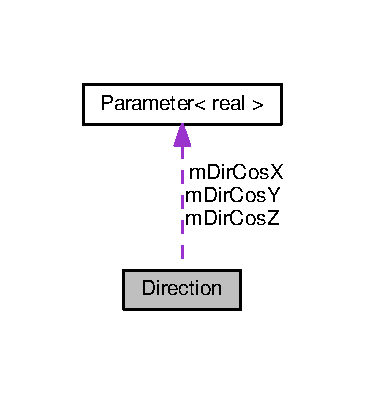
\includegraphics[width=177pt]{classDirection__coll__graph}
\end{center}
\end{figure}
\subsection*{Public Member Functions}
\begin{DoxyCompactItemize}
\item 
\hyperlink{classDirection_a735f451ae07927d4bb8b4631b5e53c0a}{Direction} (real alpha=0, real beta=0, real gamma=0)
\begin{DoxyCompactList}\small\item\em construction with global coordinates \end{DoxyCompactList}\end{DoxyCompactItemize}
\subsection*{Protected Attributes}
\begin{DoxyCompactItemize}
\item 
\hyperlink{classParameter}{Parameter}$<$ real $>$ \hyperlink{classDirection_a796f5d3ab9275f9711e8454c1852e8a3}{m\+Dir\+CosX}\hypertarget{classDirection_a796f5d3ab9275f9711e8454c1852e8a3}{}\label{classDirection_a796f5d3ab9275f9711e8454c1852e8a3}

\begin{DoxyCompactList}\small\item\em direction cosine x-\/axis in global coordinate system \end{DoxyCompactList}\item 
\hyperlink{classParameter}{Parameter}$<$ real $>$ \hyperlink{classDirection_a7a857846b71b40148a2058deeedd7c56}{m\+Dir\+CosY}\hypertarget{classDirection_a7a857846b71b40148a2058deeedd7c56}{}\label{classDirection_a7a857846b71b40148a2058deeedd7c56}

\begin{DoxyCompactList}\small\item\em direction cosine y-\/axis in global coordinate system \end{DoxyCompactList}\item 
\hyperlink{classParameter}{Parameter}$<$ real $>$ \hyperlink{classDirection_a15cd63604eccaaec032691871a316396}{m\+Dir\+CosZ}\hypertarget{classDirection_a15cd63604eccaaec032691871a316396}{}\label{classDirection_a15cd63604eccaaec032691871a316396}

\begin{DoxyCompactList}\small\item\em direction cosine z-\/axis in global coordinate system \end{DoxyCompactList}\end{DoxyCompactItemize}


\subsection{Detailed Description}
\hyperlink{classDirection}{Direction} manages Directions/\+Orientations in Space. 

This is the basic class for representing the direction (e.\+g. of a ray). The direction can be given, of course, in different coordinate systems and with different representations which have different advantages. However, it is internally stored in \char`\"{}the\char`\"{} one and only global coordinate system. in the direction cosine way. Methods for obtaining the direction in other systems and other representation are given. Angles are given in radians.

\begin{DoxyDate}{Date}
07.\+4.\+2017 
\end{DoxyDate}
\begin{DoxyAuthor}{Author}
Tobias Haist (\href{mailto:haist@ito.uni-stuttgart.de}{\tt haist@ito.\+uni-\/stuttgart.\+de}) 
\end{DoxyAuthor}


\subsection{Constructor \& Destructor Documentation}
\index{Direction@{Direction}!Direction@{Direction}}
\index{Direction@{Direction}!Direction@{Direction}}
\subsubsection[{\texorpdfstring{Direction(real alpha=0, real beta=0, real gamma=0)}{Direction(real alpha=0, real beta=0, real gamma=0)}}]{\setlength{\rightskip}{0pt plus 5cm}Direction\+::\+Direction (
\begin{DoxyParamCaption}
\item[{real}]{alpha = {\ttfamily 0}, }
\item[{real}]{beta = {\ttfamily 0}, }
\item[{real}]{gamma = {\ttfamily 0}}
\end{DoxyParamCaption}
)}\hypertarget{classDirection_a735f451ae07927d4bb8b4631b5e53c0a}{}\label{classDirection_a735f451ae07927d4bb8b4631b5e53c0a}


construction with global coordinates 


\begin{DoxyParams}{Parameters}
{\em a} & global direction cosine with respect to x axis \\
\hline
{\em b} & global direction cosine with respect to y axis \\
\hline
{\em c} & global direction cosine with respect to z axis \\
\hline
\end{DoxyParams}


The documentation for this class was generated from the following files\+:\begin{DoxyCompactItemize}
\item 
\hyperlink{direction_8h}{direction.\+h}\item 
direction.\+cc\end{DoxyCompactItemize}

\hypertarget{classElement}{}\section{Element Class Reference}
\label{classElement}\index{Element@{Element}}


\hyperlink{classElement}{Element} represents an element/component of an optical system.  




{\ttfamily \#include $<$element.\+h$>$}



Inheritance diagram for Element\+:\nopagebreak
\begin{figure}[H]
\begin{center}
\leavevmode
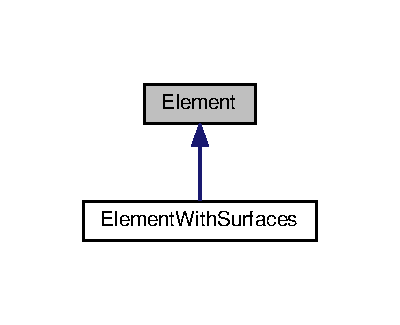
\includegraphics[width=192pt]{classElement__inherit__graph}
\end{center}
\end{figure}


Collaboration diagram for Element\+:
\nopagebreak
\begin{figure}[H]
\begin{center}
\leavevmode
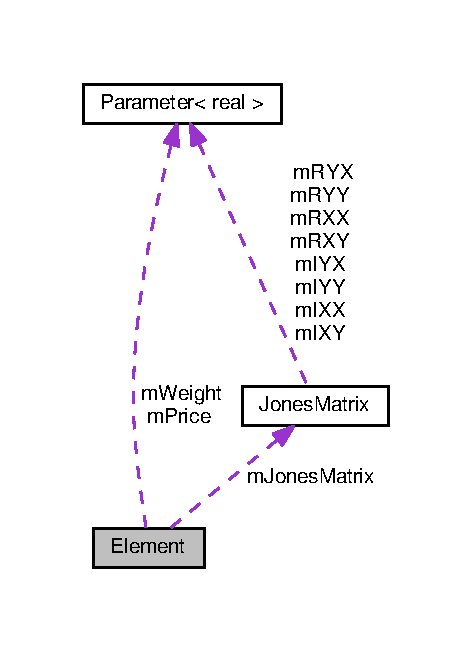
\includegraphics[width=227pt]{classElement__coll__graph}
\end{center}
\end{figure}
\subsection*{Public Member Functions}
\begin{DoxyCompactItemize}
\item 
\hyperlink{classElement_ab0d0e20be9a36ae676202db753faeec9}{Element} ()\hypertarget{classElement_ab0d0e20be9a36ae676202db753faeec9}{}\label{classElement_ab0d0e20be9a36ae676202db753faeec9}

\begin{DoxyCompactList}\small\item\em ctor \end{DoxyCompactList}\item 
virtual \hyperlink{classElement_a13d54ba9c08b6bec651402f1c2bb002c}{$\sim$\+Element} ()\hypertarget{classElement_a13d54ba9c08b6bec651402f1c2bb002c}{}\label{classElement_a13d54ba9c08b6bec651402f1c2bb002c}

\begin{DoxyCompactList}\small\item\em dtor \end{DoxyCompactList}\end{DoxyCompactItemize}
\subsection*{Protected Attributes}
\begin{DoxyCompactItemize}
\item 
\hyperlink{classParameter}{Parameter}$<$ real $>$ \hyperlink{classElement_a69ec3816139f3e3664ddc8ee7686406d}{m\+Weight}\hypertarget{classElement_a69ec3816139f3e3664ddc8ee7686406d}{}\label{classElement_a69ec3816139f3e3664ddc8ee7686406d}

\begin{DoxyCompactList}\small\item\em Weight of element in g. \end{DoxyCompactList}\item 
\hyperlink{classParameter}{Parameter}$<$ real $>$ \hyperlink{classElement_a0ba80b79bb7b1280510eb9f66eda786b}{m\+Price}\hypertarget{classElement_a0ba80b79bb7b1280510eb9f66eda786b}{}\label{classElement_a0ba80b79bb7b1280510eb9f66eda786b}

\begin{DoxyCompactList}\small\item\em Price of element in Euro. \end{DoxyCompactList}\item 
\hyperlink{classJonesMatrix}{Jones\+Matrix} $\ast$ \hyperlink{classElement_a62fb95690c351f1adb1bb642f8f6d150}{m\+Jones\+Matrix}\hypertarget{classElement_a62fb95690c351f1adb1bb642f8f6d150}{}\label{classElement_a62fb95690c351f1adb1bb642f8f6d150}

\begin{DoxyCompactList}\small\item\em Pointer to a Jones Matrix or N\+U\+LL. \end{DoxyCompactList}\end{DoxyCompactItemize}


\subsection{Detailed Description}
\hyperlink{classElement}{Element} represents an element/component of an optical system. 

In Trace\+Open Elements are the building blocks of optical systems. A typical element might be a lens which might consist of multiple surfaces. An element might also be a \char`\"{}group\char`\"{} of lenses or other things like a scattering volume.

\begin{DoxyDate}{Date}
07.\+4.\+2017 
\end{DoxyDate}
\begin{DoxyAuthor}{Author}
Tobias Haist (\href{mailto:haist@ito.uni-stuttgart.de}{\tt haist@ito.\+uni-\/stuttgart.\+de}) 
\end{DoxyAuthor}


The documentation for this class was generated from the following files\+:\begin{DoxyCompactItemize}
\item 
\hyperlink{element_8h}{element.\+h}\item 
\hyperlink{element_8cc}{element.\+cc}\end{DoxyCompactItemize}

\hypertarget{classElementWithSurfaces}{}\section{Element\+With\+Surfaces Class Reference}
\label{classElementWithSurfaces}\index{Element\+With\+Surfaces@{Element\+With\+Surfaces}}


\hyperlink{classElementWithSurfaces}{Element\+With\+Surfaces} represents things like typical lenses.  




{\ttfamily \#include $<$elementwithsurfaces.\+h$>$}



Inheritance diagram for Element\+With\+Surfaces\+:\nopagebreak
\begin{figure}[H]
\begin{center}
\leavevmode
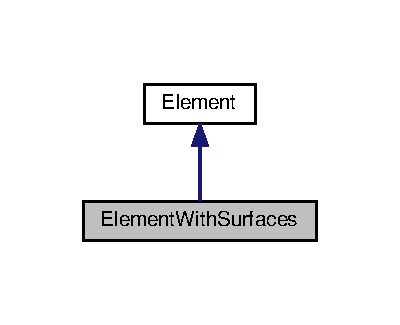
\includegraphics[width=192pt]{classElementWithSurfaces__inherit__graph}
\end{center}
\end{figure}


Collaboration diagram for Element\+With\+Surfaces\+:
\nopagebreak
\begin{figure}[H]
\begin{center}
\leavevmode
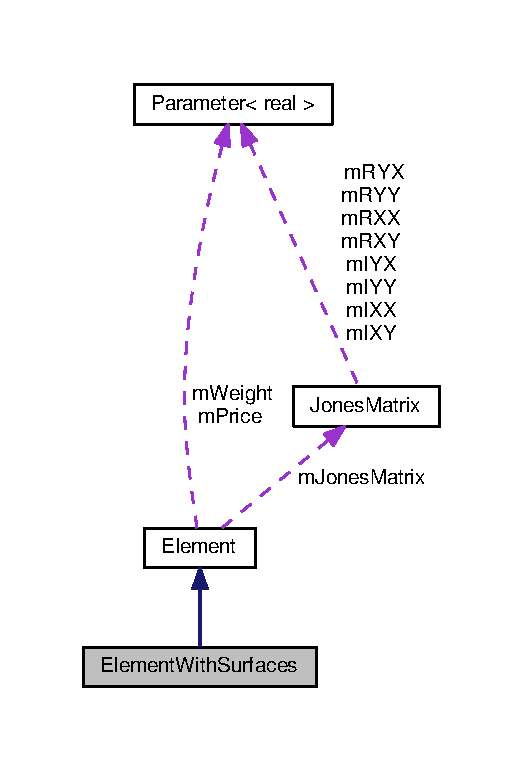
\includegraphics[width=251pt]{classElementWithSurfaces__coll__graph}
\end{center}
\end{figure}
\subsection*{Public Member Functions}
\begin{DoxyCompactItemize}
\item 
\hyperlink{classElementWithSurfaces_a0d27f004d13a2b81a8ee2b8adba48ea0}{Element\+With\+Surfaces} ()\hypertarget{classElementWithSurfaces_a0d27f004d13a2b81a8ee2b8adba48ea0}{}\label{classElementWithSurfaces_a0d27f004d13a2b81a8ee2b8adba48ea0}

\begin{DoxyCompactList}\small\item\em ctor \end{DoxyCompactList}\item 
\hyperlink{classElementWithSurfaces_a361ebb826758c49bf2de1671bcc861ec}{$\sim$\+Element\+With\+Surfaces} ()\hypertarget{classElementWithSurfaces_a361ebb826758c49bf2de1671bcc861ec}{}\label{classElementWithSurfaces_a361ebb826758c49bf2de1671bcc861ec}

\begin{DoxyCompactList}\small\item\em dtor \end{DoxyCompactList}\item 
void \hyperlink{classElementWithSurfaces_aa884a6c58261c3fb4143785b9bec613e}{add\+Surface} (\hyperlink{classSurface}{Surface} $\ast$const s, \hyperlink{classMaterial}{Material} $\ast$const m)
\begin{DoxyCompactList}\small\item\em add a surface at the end of m\+Surfaces \end{DoxyCompactList}\item 
void \hyperlink{classElementWithSurfaces_a1a80e23ffdde5afe3ae94c105bb0b1ba}{standard\+Lens} (real r1, real r2, real thickness, \hyperlink{classMaterial}{Material} $\ast$const material, real diameter=0)
\begin{DoxyCompactList}\small\item\em create a standard lens \end{DoxyCompactList}\item 
void \hyperlink{classElementWithSurfaces_a32df06ede6cfea6425e68037b69c4dab}{achromat} (real r1, real r2, real r3, real thickness1, real thickness2, \hyperlink{classMaterial}{Material} $\ast$const m1, \hyperlink{classMaterial}{Material} $\ast$const m2, real diameter=0)
\begin{DoxyCompactList}\small\item\em create an achromat \end{DoxyCompactList}\end{DoxyCompactItemize}
\subsection*{Protected Attributes}
\begin{DoxyCompactItemize}
\item 
int \hyperlink{classElementWithSurfaces_a86e3872cf6bd9b6bb3d5d9b504dbbaa8}{m\+Cnt\+Surfaces}\hypertarget{classElementWithSurfaces_a86e3872cf6bd9b6bb3d5d9b504dbbaa8}{}\label{classElementWithSurfaces_a86e3872cf6bd9b6bb3d5d9b504dbbaa8}

\begin{DoxyCompactList}\small\item\em number of surfaces \end{DoxyCompactList}\item 
std\+::vector$<$ \hyperlink{classSurface}{Surface} $\ast$ $>$ \hyperlink{classElementWithSurfaces_a3fb5888bb6ec5de9d7fe81bbbc2d2afd}{m\+Surfaces}\hypertarget{classElementWithSurfaces_a3fb5888bb6ec5de9d7fe81bbbc2d2afd}{}\label{classElementWithSurfaces_a3fb5888bb6ec5de9d7fe81bbbc2d2afd}

\begin{DoxyCompactList}\small\item\em All surfaces that make the element. \end{DoxyCompactList}\item 
std\+::vector$<$ \hyperlink{classMaterial}{Material} $\ast$ $>$ \hyperlink{classElementWithSurfaces_af2900bba23d0aa0bdc38f69dcc00e086}{m\+Materials}\hypertarget{classElementWithSurfaces_af2900bba23d0aa0bdc38f69dcc00e086}{}\label{classElementWithSurfaces_af2900bba23d0aa0bdc38f69dcc00e086}

\begin{DoxyCompactList}\small\item\em \hyperlink{classMaterial}{Material} between successive surfaces. \end{DoxyCompactList}\end{DoxyCompactItemize}


\subsection{Detailed Description}
\hyperlink{classElementWithSurfaces}{Element\+With\+Surfaces} represents things like typical lenses. 

Most often, elements are lenses or mirrors. These elements are \char`\"{}elements with (or consisting of) surfaces\char`\"{}.

We might in the future have elements with L\+O\+TS of surfaces, e.\+g. in order to simulate quasi continuos changes. Therefore, it would not be memory efficient to always have an \hyperlink{classArray}{Array} (of pointers) e.\+g. with 10.\+000 entries for every \hyperlink{classElementWithSurfaces}{Element\+With\+Surfaces}. Therefore we use a container ( vector$<$\+Surface$\ast$$>$ )(

\begin{DoxyDate}{Date}
07.\+4.\+2017 
\end{DoxyDate}
\begin{DoxyAuthor}{Author}
Tobias Haist (\href{mailto:haist@ito.uni-stuttgart.de}{\tt haist@ito.\+uni-\/stuttgart.\+de}) 
\end{DoxyAuthor}


\subsection{Member Function Documentation}
\index{Element\+With\+Surfaces@{Element\+With\+Surfaces}!achromat@{achromat}}
\index{achromat@{achromat}!Element\+With\+Surfaces@{Element\+With\+Surfaces}}
\subsubsection[{\texorpdfstring{achromat(real r1, real r2, real r3, real thickness1, real thickness2, Material $\ast$const m1, Material $\ast$const m2, real diameter=0)}{achromat(real r1, real r2, real r3, real thickness1, real thickness2, Material *const m1, Material *const m2, real diameter=0)}}]{\setlength{\rightskip}{0pt plus 5cm}void Element\+With\+Surfaces\+::achromat (
\begin{DoxyParamCaption}
\item[{real}]{r1, }
\item[{real}]{r2, }
\item[{real}]{r3, }
\item[{real}]{thickness1, }
\item[{real}]{thickness2, }
\item[{{\bf Material} $\ast$const}]{m1, }
\item[{{\bf Material} $\ast$const}]{m2, }
\item[{real}]{diameter = {\ttfamily 0}}
\end{DoxyParamCaption}
)}\hypertarget{classElementWithSurfaces_a32df06ede6cfea6425e68037b69c4dab}{}\label{classElementWithSurfaces_a32df06ede6cfea6425e68037b69c4dab}


create an achromat 


\begin{DoxyParams}{Parameters}
{\em r1} & radius of curvature surface 1 \\
\hline
{\em r2} & radius of curvature surface 2 \\
\hline
{\em r3} & radius of curvature surface 3 \\
\hline
{\em thickness1} & thickness between surface 1 and 2 \\
\hline
{\em thickness2} & thickness between surface 2 and 3 \\
\hline
{\em m1} & Pointer to material 1 \\
\hline
{\em mw} & Pointer to material 2 \\
\hline
{\em diameter} & lens diameter \\
\hline
\end{DoxyParams}
\index{Element\+With\+Surfaces@{Element\+With\+Surfaces}!add\+Surface@{add\+Surface}}
\index{add\+Surface@{add\+Surface}!Element\+With\+Surfaces@{Element\+With\+Surfaces}}
\subsubsection[{\texorpdfstring{add\+Surface(\+Surface $\ast$const s, Material $\ast$const m)}{addSurface(Surface *const s, Material *const m)}}]{\setlength{\rightskip}{0pt plus 5cm}void Element\+With\+Surfaces\+::add\+Surface (
\begin{DoxyParamCaption}
\item[{{\bf Surface} $\ast$const}]{s, }
\item[{{\bf Material} $\ast$const}]{m}
\end{DoxyParamCaption}
)}\hypertarget{classElementWithSurfaces_aa884a6c58261c3fb4143785b9bec613e}{}\label{classElementWithSurfaces_aa884a6c58261c3fb4143785b9bec613e}


add a surface at the end of m\+Surfaces 


\begin{DoxyParams}{Parameters}
{\em s} & Pointer to surface \\
\hline
{\em m} & Pointer to material \\
\hline
\end{DoxyParams}
\index{Element\+With\+Surfaces@{Element\+With\+Surfaces}!standard\+Lens@{standard\+Lens}}
\index{standard\+Lens@{standard\+Lens}!Element\+With\+Surfaces@{Element\+With\+Surfaces}}
\subsubsection[{\texorpdfstring{standard\+Lens(real r1, real r2, real thickness, Material $\ast$const material, real diameter=0)}{standardLens(real r1, real r2, real thickness, Material *const material, real diameter=0)}}]{\setlength{\rightskip}{0pt plus 5cm}void Element\+With\+Surfaces\+::standard\+Lens (
\begin{DoxyParamCaption}
\item[{real}]{r1, }
\item[{real}]{r2, }
\item[{real}]{thickness, }
\item[{{\bf Material} $\ast$const}]{material, }
\item[{real}]{diameter = {\ttfamily 0}}
\end{DoxyParamCaption}
)}\hypertarget{classElementWithSurfaces_a1a80e23ffdde5afe3ae94c105bb0b1ba}{}\label{classElementWithSurfaces_a1a80e23ffdde5afe3ae94c105bb0b1ba}


create a standard lens 


\begin{DoxyParams}{Parameters}
{\em r1} & radius of curvature surface 1 \\
\hline
{\em r2} & radius of curvature surface 2 \\
\hline
{\em thickness} & thickness between surface 1 and 2 \\
\hline
{\em material} & Pointer to material \\
\hline
{\em diameter} & lens diameter \\
\hline
\end{DoxyParams}


The documentation for this class was generated from the following files\+:\begin{DoxyCompactItemize}
\item 
\hyperlink{elementwithsurfaces_8h}{elementwithsurfaces.\+h}\item 
\hyperlink{elementwithsurfaces_8cc}{elementwithsurfaces.\+cc}\end{DoxyCompactItemize}

\hypertarget{classEnvironment}{}\section{Environment Class Reference}
\label{classEnvironment}\index{Environment@{Environment}}


Enviroment is responsible for storing/computing enviromental parameters.  




{\ttfamily \#include $<$environment.\+h$>$}



Collaboration diagram for Environment\+:
\nopagebreak
\begin{figure}[H]
\begin{center}
\leavevmode
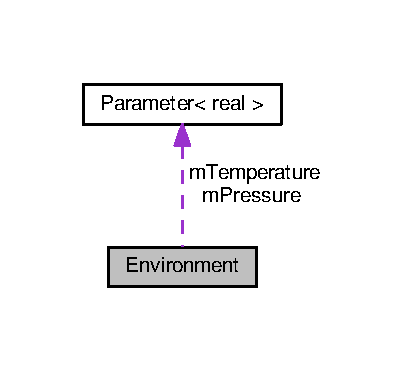
\includegraphics[width=195pt]{classEnvironment__coll__graph}
\end{center}
\end{figure}
\subsection*{Public Member Functions}
\begin{DoxyCompactItemize}
\item 
\hyperlink{classEnvironment_a61012e8e0cfa5b8181e715a96211c2d8}{Environment} (real temperature, real pressure)
\begin{DoxyCompactList}\small\item\em ctor \end{DoxyCompactList}\item 
real \hyperlink{classEnvironment_a520f5872c242108b6dc06a9c06859516}{get\+Temperature} () const 
\begin{DoxyCompactList}\small\item\em get function \end{DoxyCompactList}\item 
void \hyperlink{classEnvironment_af7c2756f2d541b69f75234ccc5a5aa2c}{set\+Temperature} (real temperature)\hypertarget{classEnvironment_af7c2756f2d541b69f75234ccc5a5aa2c}{}\label{classEnvironment_af7c2756f2d541b69f75234ccc5a5aa2c}

\begin{DoxyCompactList}\small\item\em set function \end{DoxyCompactList}\end{DoxyCompactItemize}
\subsection*{Protected Attributes}
\begin{DoxyCompactItemize}
\item 
\hyperlink{classParameter}{Parameter}$<$ real $>$ \hyperlink{classEnvironment_acb54854a3e53a598dd025611452fcbf6}{m\+Temperature}\hypertarget{classEnvironment_acb54854a3e53a598dd025611452fcbf6}{}\label{classEnvironment_acb54854a3e53a598dd025611452fcbf6}

\begin{DoxyCompactList}\small\item\em Temperature in K. \end{DoxyCompactList}\item 
\hyperlink{classParameter}{Parameter}$<$ real $>$ \hyperlink{classEnvironment_ac00fba3fd29fb391618ac6276d8a5c36}{m\+Pressure}\hypertarget{classEnvironment_ac00fba3fd29fb391618ac6276d8a5c36}{}\label{classEnvironment_ac00fba3fd29fb391618ac6276d8a5c36}

\begin{DoxyCompactList}\small\item\em Pressure in bar. \end{DoxyCompactList}\end{DoxyCompactItemize}


\subsection{Detailed Description}
Enviroment is responsible for storing/computing enviromental parameters. 

\subsection{Constructor \& Destructor Documentation}
\index{Environment@{Environment}!Environment@{Environment}}
\index{Environment@{Environment}!Environment@{Environment}}
\subsubsection[{\texorpdfstring{Environment(real temperature, real pressure)}{Environment(real temperature, real pressure)}}]{\setlength{\rightskip}{0pt plus 5cm}Environment\+::\+Environment (
\begin{DoxyParamCaption}
\item[{real}]{temperature, }
\item[{real}]{pressure}
\end{DoxyParamCaption}
)}\hypertarget{classEnvironment_a61012e8e0cfa5b8181e715a96211c2d8}{}\label{classEnvironment_a61012e8e0cfa5b8181e715a96211c2d8}


ctor 


\begin{DoxyParams}{Parameters}
{\em n} & refractive index \\
\hline
\end{DoxyParams}


\subsection{Member Function Documentation}
\index{Environment@{Environment}!get\+Temperature@{get\+Temperature}}
\index{get\+Temperature@{get\+Temperature}!Environment@{Environment}}
\subsubsection[{\texorpdfstring{get\+Temperature() const }{getTemperature() const }}]{\setlength{\rightskip}{0pt plus 5cm}real Environment\+::get\+Temperature (
\begin{DoxyParamCaption}
{}
\end{DoxyParamCaption}
) const}\hypertarget{classEnvironment_a520f5872c242108b6dc06a9c06859516}{}\label{classEnvironment_a520f5872c242108b6dc06a9c06859516}


get function 


\begin{DoxyParams}{Parameters}
{\em n} & refractive index \\
\hline
\end{DoxyParams}


The documentation for this class was generated from the following files\+:\begin{DoxyCompactItemize}
\item 
environment.\+h\item 
\hyperlink{environment_8cc}{environment.\+cc}\end{DoxyCompactItemize}

\hypertarget{classInteraction}{}\section{Interaction Class Reference}
\label{classInteraction}\index{Interaction@{Interaction}}


Most optical components are made out of Surfaces.  




{\ttfamily \#include $<$interaction.\+h$>$}



Inheritance diagram for Interaction\+:\nopagebreak
\begin{figure}[H]
\begin{center}
\leavevmode
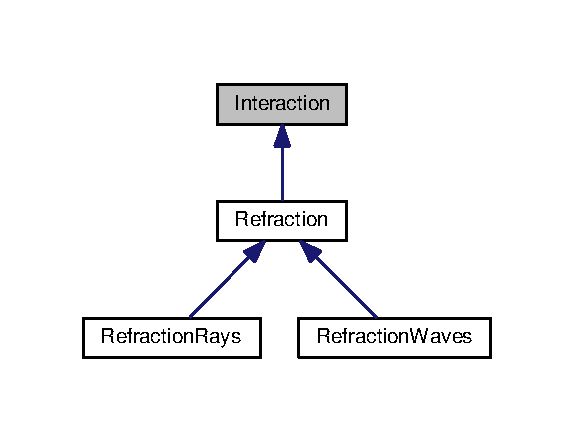
\includegraphics[width=276pt]{classInteraction__inherit__graph}
\end{center}
\end{figure}


Collaboration diagram for Interaction\+:\nopagebreak
\begin{figure}[H]
\begin{center}
\leavevmode
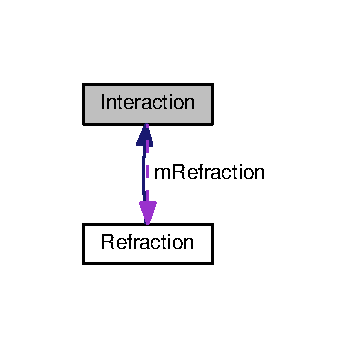
\includegraphics[width=168pt]{classInteraction__coll__graph}
\end{center}
\end{figure}
\subsection*{Public Member Functions}
\begin{DoxyCompactItemize}
\item 
\hyperlink{classInteraction_aadfd0e254296043c26508d47090ace76}{Interaction} ()\hypertarget{classInteraction_aadfd0e254296043c26508d47090ace76}{}\label{classInteraction_aadfd0e254296043c26508d47090ace76}

\begin{DoxyCompactList}\small\item\em dtor \end{DoxyCompactList}\item 
virtual \hyperlink{classInteraction_a6610199fedc7fae617003cb2f397c825}{$\sim$\+Interaction} ()\hypertarget{classInteraction_a6610199fedc7fae617003cb2f397c825}{}\label{classInteraction_a6610199fedc7fae617003cb2f397c825}

\begin{DoxyCompactList}\small\item\em dtor \end{DoxyCompactList}\item 
void \hyperlink{classInteraction_a97cbbf080cda868a35f80cfbe7e673f5}{set\+Global\+Interactions} (\hyperlink{classLight}{Light} $\ast$const light)
\begin{DoxyCompactList}\small\item\em set global interactions according to light modell \end{DoxyCompactList}\end{DoxyCompactItemize}
\subsection*{Public Attributes}
\begin{DoxyCompactItemize}
\item 
\hyperlink{classRefraction}{Refraction} $\ast$ \hyperlink{classInteraction_a80f9aba433c1c701b1e1545372c25c20}{m\+Refraction}\hypertarget{classInteraction_a80f9aba433c1c701b1e1545372c25c20}{}\label{classInteraction_a80f9aba433c1c701b1e1545372c25c20}

\begin{DoxyCompactList}\small\item\em this is what we call when refraction occurs \end{DoxyCompactList}\end{DoxyCompactItemize}


\subsection{Detailed Description}
Most optical components are made out of Surfaces. 

The abstract base class \hyperlink{classInteraction}{Interaction} is the main class that is responsible for interactions like refraction, refraction etc.

\begin{DoxyDate}{Date}
15.\+4.\+2017 
\end{DoxyDate}
\begin{DoxyAuthor}{Author}
Tobias Haist (\href{mailto:haist@ito.uni-stuttgart.de}{\tt haist@ito.\+uni-\/stuttgart.\+de}) 
\end{DoxyAuthor}


\subsection{Member Function Documentation}
\index{Interaction@{Interaction}!set\+Global\+Interactions@{set\+Global\+Interactions}}
\index{set\+Global\+Interactions@{set\+Global\+Interactions}!Interaction@{Interaction}}
\subsubsection[{\texorpdfstring{set\+Global\+Interactions(\+Light $\ast$const light)}{setGlobalInteractions(Light *const light)}}]{\setlength{\rightskip}{0pt plus 5cm}void Interaction\+::set\+Global\+Interactions (
\begin{DoxyParamCaption}
\item[{{\bf Light} $\ast$const}]{light}
\end{DoxyParamCaption}
)}\hypertarget{classInteraction_a97cbbf080cda868a35f80cfbe7e673f5}{}\label{classInteraction_a97cbbf080cda868a35f80cfbe7e673f5}


set global interactions according to light modell 


\begin{DoxyParams}{Parameters}
{\em light} & light model to be used for global interactions \\
\hline
\end{DoxyParams}


The documentation for this class was generated from the following files\+:\begin{DoxyCompactItemize}
\item 
\hyperlink{interaction_8h}{interaction.\+h}\item 
\hyperlink{interaction_8cc}{interaction.\+cc}\end{DoxyCompactItemize}

\hypertarget{classJonesMatrix}{}\section{Jones\+Matrix Class Reference}
\label{classJonesMatrix}\index{Jones\+Matrix@{Jones\+Matrix}}


\hyperlink{classJonesMatrix}{Jones\+Matrix} is just the Jones matrix of an element.  




{\ttfamily \#include $<$jonesmatrix.\+h$>$}



Collaboration diagram for Jones\+Matrix\+:
\nopagebreak
\begin{figure}[H]
\begin{center}
\leavevmode
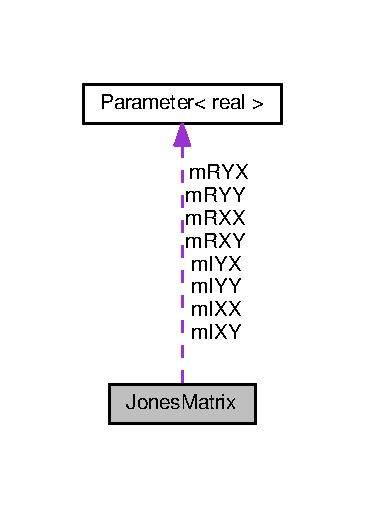
\includegraphics[width=175pt]{classJonesMatrix__coll__graph}
\end{center}
\end{figure}
\subsection*{Public Member Functions}
\begin{DoxyCompactItemize}
\item 
\hyperlink{classJonesMatrix_a7fc6346ea0046fe0424fac0401965014}{Jones\+Matrix} (real ra, real ia, real rb, real ib, real rc, real ic, real rd, real id)
\end{DoxyCompactItemize}
\subsection*{Protected Attributes}
\begin{DoxyCompactItemize}
\item 
\hyperlink{classParameter}{Parameter}$<$ real $>$ \hyperlink{classJonesMatrix_ac09049ab42066f907ab293f95fbcf577}{m\+R\+XX}\hypertarget{classJonesMatrix_ac09049ab42066f907ab293f95fbcf577}{}\label{classJonesMatrix_ac09049ab42066f907ab293f95fbcf577}

\begin{DoxyCompactList}\small\item\em real part \hyperlink{classElement}{Element} a (xx) \end{DoxyCompactList}\item 
\hyperlink{classParameter}{Parameter}$<$ real $>$ \hyperlink{classJonesMatrix_a204a58a2b4d54a0df6054a4358156125}{m\+I\+XX}\hypertarget{classJonesMatrix_a204a58a2b4d54a0df6054a4358156125}{}\label{classJonesMatrix_a204a58a2b4d54a0df6054a4358156125}

\begin{DoxyCompactList}\small\item\em imag part \hyperlink{classElement}{Element} a (xx) \end{DoxyCompactList}\item 
\hyperlink{classParameter}{Parameter}$<$ real $>$ \hyperlink{classJonesMatrix_ae3173c87735713c7837804c1aa93c2a8}{m\+R\+XY}\hypertarget{classJonesMatrix_ae3173c87735713c7837804c1aa93c2a8}{}\label{classJonesMatrix_ae3173c87735713c7837804c1aa93c2a8}

\begin{DoxyCompactList}\small\item\em real part \hyperlink{classElement}{Element} b (xy) \end{DoxyCompactList}\item 
\hyperlink{classParameter}{Parameter}$<$ real $>$ \hyperlink{classJonesMatrix_a61aef249b9d7c520ec13d40e6aa50642}{m\+I\+XY}\hypertarget{classJonesMatrix_a61aef249b9d7c520ec13d40e6aa50642}{}\label{classJonesMatrix_a61aef249b9d7c520ec13d40e6aa50642}

\begin{DoxyCompactList}\small\item\em imag part \hyperlink{classElement}{Element} b (xy) \end{DoxyCompactList}\item 
\hyperlink{classParameter}{Parameter}$<$ real $>$ \hyperlink{classJonesMatrix_ae2cc78a5511cd33933e9d6b52722c996}{m\+R\+YX}\hypertarget{classJonesMatrix_ae2cc78a5511cd33933e9d6b52722c996}{}\label{classJonesMatrix_ae2cc78a5511cd33933e9d6b52722c996}

\begin{DoxyCompactList}\small\item\em real part \hyperlink{classElement}{Element} a (yx) \end{DoxyCompactList}\item 
\hyperlink{classParameter}{Parameter}$<$ real $>$ \hyperlink{classJonesMatrix_ad19c69bc677f85490ccbfada95b9474f}{m\+I\+YX}\hypertarget{classJonesMatrix_ad19c69bc677f85490ccbfada95b9474f}{}\label{classJonesMatrix_ad19c69bc677f85490ccbfada95b9474f}

\begin{DoxyCompactList}\small\item\em imag part \hyperlink{classElement}{Element} a (yx) \end{DoxyCompactList}\item 
\hyperlink{classParameter}{Parameter}$<$ real $>$ \hyperlink{classJonesMatrix_aa3285508a9c7ad25250eb0d7511e9988}{m\+R\+YY}\hypertarget{classJonesMatrix_aa3285508a9c7ad25250eb0d7511e9988}{}\label{classJonesMatrix_aa3285508a9c7ad25250eb0d7511e9988}

\begin{DoxyCompactList}\small\item\em real part \hyperlink{classElement}{Element} a (yy) \end{DoxyCompactList}\item 
\hyperlink{classParameter}{Parameter}$<$ real $>$ \hyperlink{classJonesMatrix_a44a73c7ef4adeffe8c825618668f344f}{m\+I\+YY}\hypertarget{classJonesMatrix_a44a73c7ef4adeffe8c825618668f344f}{}\label{classJonesMatrix_a44a73c7ef4adeffe8c825618668f344f}

\begin{DoxyCompactList}\small\item\em imag part \hyperlink{classElement}{Element} a (yy) \end{DoxyCompactList}\end{DoxyCompactItemize}


\subsection{Detailed Description}
\hyperlink{classJonesMatrix}{Jones\+Matrix} is just the Jones matrix of an element. 

In Trace\+Open polarized light is represented using Jones matrices

\begin{DoxyDate}{Date}
07.\+4.\+2017 
\end{DoxyDate}
\begin{DoxyAuthor}{Author}
Tobias Haist (\href{mailto:haist@ito.uni-stuttgart.de}{\tt haist@ito.\+uni-\/stuttgart.\+de}) 
\end{DoxyAuthor}


\subsection{Constructor \& Destructor Documentation}
\index{Jones\+Matrix@{Jones\+Matrix}!Jones\+Matrix@{Jones\+Matrix}}
\index{Jones\+Matrix@{Jones\+Matrix}!Jones\+Matrix@{Jones\+Matrix}}
\subsubsection[{\texorpdfstring{Jones\+Matrix(real ra, real ia, real rb, real ib, real rc, real ic, real rd, real id)}{JonesMatrix(real ra, real ia, real rb, real ib, real rc, real ic, real rd, real id)}}]{\setlength{\rightskip}{0pt plus 5cm}Jones\+Matrix\+::\+Jones\+Matrix (
\begin{DoxyParamCaption}
\item[{real}]{ra, }
\item[{real}]{ia, }
\item[{real}]{rb, }
\item[{real}]{ib, }
\item[{real}]{rc, }
\item[{real}]{ic, }
\item[{real}]{rd, }
\item[{real}]{id}
\end{DoxyParamCaption}
)}\hypertarget{classJonesMatrix_a7fc6346ea0046fe0424fac0401965014}{}\label{classJonesMatrix_a7fc6346ea0046fe0424fac0401965014}

\begin{DoxyParams}{Parameters}
{\em e} & Pointer to \hyperlink{classElement}{Element} to be added to end of list \\
\hline
\end{DoxyParams}


The documentation for this class was generated from the following files\+:\begin{DoxyCompactItemize}
\item 
\hyperlink{jonesmatrix_8h}{jonesmatrix.\+h}\item 
\hyperlink{jonesmatrix_8cc}{jonesmatrix.\+cc}\end{DoxyCompactItemize}

\hypertarget{classLight}{}\section{Light Class Reference}
\label{classLight}\index{Light@{Light}}


Inheritance diagram for Light\+:\nopagebreak
\begin{figure}[H]
\begin{center}
\leavevmode
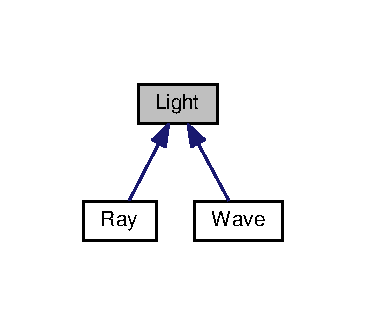
\includegraphics[width=176pt]{classLight__inherit__graph}
\end{center}
\end{figure}


Collaboration diagram for Light\+:\nopagebreak
\begin{figure}[H]
\begin{center}
\leavevmode
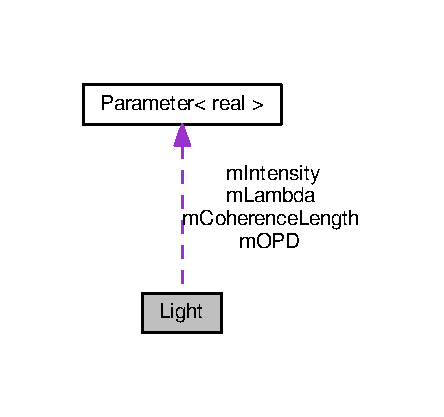
\includegraphics[width=213pt]{classLight__coll__graph}
\end{center}
\end{figure}
\subsection*{Public Member Functions}
\begin{DoxyCompactItemize}
\item 
\hyperlink{classLight_aa3c2e043724b07ece1e11732472b9520}{Light} (\hyperlink{light_8h_a6dc57eac1ae8b19466de554123d5c6c3}{type\+Light} type, real lambda, real intensity)
\begin{DoxyCompactList}\small\item\em ctor \end{DoxyCompactList}\item 
void \hyperlink{classLight_ad23d1727356fae1075d82f5e9596f886}{set\+Position} (\hyperlink{classPoint}{Point} p)\hypertarget{classLight_ad23d1727356fae1075d82f5e9596f886}{}\label{classLight_ad23d1727356fae1075d82f5e9596f886}

\begin{DoxyCompactList}\small\item\em sets the startposition of the light \end{DoxyCompactList}\item 
\hyperlink{light_8h_a6dc57eac1ae8b19466de554123d5c6c3}{type\+Light} {\bfseries get\+Type} () const \hypertarget{classLight_a8571ce69ae09c26937733d435c0d0276}{}\label{classLight_a8571ce69ae09c26937733d435c0d0276}

\item 
bool \hyperlink{classLight_aa5371398a56853b58e9eaf87ca418bac}{is\+Alive} () const 
\begin{DoxyCompactList}\small\item\em true -\/$>$ \hyperlink{classLight}{Light} is still alive (not vignetted) \end{DoxyCompactList}\end{DoxyCompactItemize}
\subsection*{Protected Attributes}
\begin{DoxyCompactItemize}
\item 
\hyperlink{light_8h_a6dc57eac1ae8b19466de554123d5c6c3}{type\+Light} \hyperlink{classLight_aee4380e879fac1a8687c8dc4a8401d8d}{m\+Light\+Type}\hypertarget{classLight_aee4380e879fac1a8687c8dc4a8401d8d}{}\label{classLight_aee4380e879fac1a8687c8dc4a8401d8d}

\begin{DoxyCompactList}\small\item\em what kind of \hyperlink{classLight}{Light} (subclass) \end{DoxyCompactList}\item 
\hyperlink{classParameter}{Parameter}$<$ real $>$ \hyperlink{classLight_a6bcf65e42bbe7525e704edd9b22892f8}{m\+Lambda}\hypertarget{classLight_a6bcf65e42bbe7525e704edd9b22892f8}{}\label{classLight_a6bcf65e42bbe7525e704edd9b22892f8}

\begin{DoxyCompactList}\small\item\em Wavelength in m. \end{DoxyCompactList}\item 
\hyperlink{classParameter}{Parameter}$<$ real $>$ \hyperlink{classLight_a67e9a5774841ce868a7cf5b9312c6850}{m\+Coherence\+Length}\hypertarget{classLight_a67e9a5774841ce868a7cf5b9312c6850}{}\label{classLight_a67e9a5774841ce868a7cf5b9312c6850}

\begin{DoxyCompactList}\small\item\em coherence length in m \end{DoxyCompactList}\item 
\hyperlink{classParameter}{Parameter}$<$ real $>$ \hyperlink{classLight_accb9c61fcc083de4cd5a33e02347712b}{m\+Intensity}\hypertarget{classLight_accb9c61fcc083de4cd5a33e02347712b}{}\label{classLight_accb9c61fcc083de4cd5a33e02347712b}

\begin{DoxyCompactList}\small\item\em power per m$^\wedge$2 = intensity in W/m$^\wedge$2 \end{DoxyCompactList}\item 
\hyperlink{classParameter}{Parameter}$<$ real $>$ \hyperlink{classLight_a6de046378d4fa3eac06bf4cb3549e95e}{m\+O\+PD}\hypertarget{classLight_a6de046378d4fa3eac06bf4cb3549e95e}{}\label{classLight_a6de046378d4fa3eac06bf4cb3549e95e}

\begin{DoxyCompactList}\small\item\em optical path difference \end{DoxyCompactList}\item 
bool \hyperlink{classLight_a5769177ada731b92c917853ea2eb52f5}{m\+Alive}\hypertarget{classLight_a5769177ada731b92c917853ea2eb52f5}{}\label{classLight_a5769177ada731b92c917853ea2eb52f5}

\begin{DoxyCompactList}\small\item\em true -\/$>$ light still alive \end{DoxyCompactList}\end{DoxyCompactItemize}


\subsection{Constructor \& Destructor Documentation}
\index{Light@{Light}!Light@{Light}}
\index{Light@{Light}!Light@{Light}}
\subsubsection[{\texorpdfstring{Light(type\+Light type, real lambda, real intensity)}{Light(typeLight type, real lambda, real intensity)}}]{\setlength{\rightskip}{0pt plus 5cm}Light\+::\+Light (
\begin{DoxyParamCaption}
\item[{{\bf type\+Light}}]{type, }
\item[{real}]{lambda, }
\item[{real}]{intensity}
\end{DoxyParamCaption}
)}\hypertarget{classLight_aa3c2e043724b07ece1e11732472b9520}{}\label{classLight_aa3c2e043724b07ece1e11732472b9520}


ctor 


\begin{DoxyParams}{Parameters}
{\em t} & type of light \\
\hline
{\em lambda} & wavelength (in m) \\
\hline
{\em intensity} & intesity in W/m$^\wedge$2 \\
\hline
\end{DoxyParams}


\subsection{Member Function Documentation}
\index{Light@{Light}!is\+Alive@{is\+Alive}}
\index{is\+Alive@{is\+Alive}!Light@{Light}}
\subsubsection[{\texorpdfstring{is\+Alive() const }{isAlive() const }}]{\setlength{\rightskip}{0pt plus 5cm}bool Light\+::is\+Alive (
\begin{DoxyParamCaption}
{}
\end{DoxyParamCaption}
) const}\hypertarget{classLight_aa5371398a56853b58e9eaf87ca418bac}{}\label{classLight_aa5371398a56853b58e9eaf87ca418bac}


true -\/$>$ \hyperlink{classLight}{Light} is still alive (not vignetted) 

\begin{DoxyReturn}{Returns}
true -\/$>$ ray is alive (not vignetted) 
\end{DoxyReturn}


The documentation for this class was generated from the following files\+:\begin{DoxyCompactItemize}
\item 
\hyperlink{light_8h}{light.\+h}\item 
\hyperlink{light_8cc}{light.\+cc}\end{DoxyCompactItemize}

\hypertarget{classMaterial}{}\section{Material Class Reference}
\label{classMaterial}\index{Material@{Material}}


\hyperlink{classMaterial}{Material} is an abstract base calls that represents all Materials.  




{\ttfamily \#include $<$material.\+h$>$}



Inheritance diagram for Material\+:
\nopagebreak
\begin{figure}[H]
\begin{center}
\leavevmode
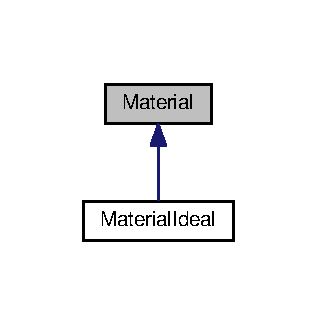
\includegraphics[width=152pt]{classMaterial__inherit__graph}
\end{center}
\end{figure}


Collaboration diagram for Material\+:
\nopagebreak
\begin{figure}[H]
\begin{center}
\leavevmode
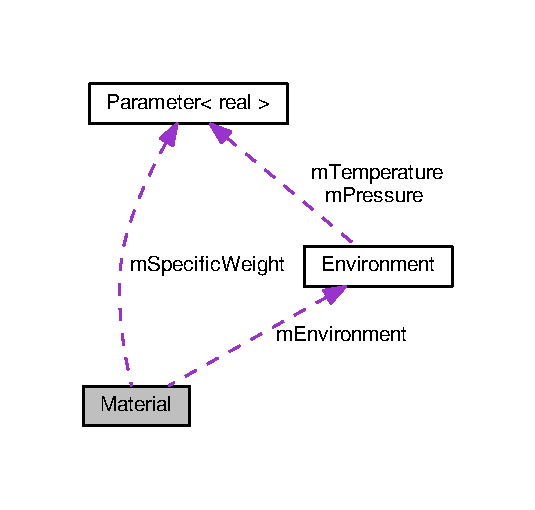
\includegraphics[width=257pt]{classMaterial__coll__graph}
\end{center}
\end{figure}
\subsection*{Public Member Functions}
\begin{DoxyCompactItemize}
\item 
\hyperlink{classMaterial_a6ae071c7815f931869131bba5414cefd}{Material} (std\+::string name, \hyperlink{classEnvironment}{Environment} $\ast$env=0, real specificic\+Weight=0)
\begin{DoxyCompactList}\small\item\em ctor \end{DoxyCompactList}\item 
virtual \hyperlink{classMaterial_a2c19452d71f54075df8f5405b03129f4}{$\sim$\+Material} ()
\begin{DoxyCompactList}\small\item\em dtor \end{DoxyCompactList}\item 
virtual real \hyperlink{classMaterial_a8994560db37896679e16161a7a7cb75b}{get\+Refractive\+Index} (real wavelength, std\+::complex$<$ real $>$ ex, std\+::complex$<$ real $>$ ey, std\+::complex$<$ real $>$ ez)=0\hypertarget{classMaterial_a8994560db37896679e16161a7a7cb75b}{}\label{classMaterial_a8994560db37896679e16161a7a7cb75b}

\begin{DoxyCompactList}\small\item\em get refractive\+Index \end{DoxyCompactList}\end{DoxyCompactItemize}
\subsection*{Protected Attributes}
\begin{DoxyCompactItemize}
\item 
std\+::string \hyperlink{classMaterial_a4dc85b2e88aa30c51dda6a54f1bd2f30}{m\+Name}\hypertarget{classMaterial_a4dc85b2e88aa30c51dda6a54f1bd2f30}{}\label{classMaterial_a4dc85b2e88aa30c51dda6a54f1bd2f30}

\begin{DoxyCompactList}\small\item\em name of \hyperlink{classMaterial}{Material} \end{DoxyCompactList}\item 
\hyperlink{classParameter}{Parameter}$<$ real $>$ \hyperlink{classMaterial_a8d6bf3cf727dd81b4eac1726e0df36b0}{m\+Specific\+Weight}\hypertarget{classMaterial_a8d6bf3cf727dd81b4eac1726e0df36b0}{}\label{classMaterial_a8d6bf3cf727dd81b4eac1726e0df36b0}

\begin{DoxyCompactList}\small\item\em Dispersion. \end{DoxyCompactList}\item 
\hyperlink{classEnvironment}{Environment} $\ast$ \hyperlink{classMaterial_adb3c2440c55d8b32a19d9c246450179a}{m\+Environment}\hypertarget{classMaterial_adb3c2440c55d8b32a19d9c246450179a}{}\label{classMaterial_adb3c2440c55d8b32a19d9c246450179a}

\begin{DoxyCompactList}\small\item\em Enviromental conditions (e.\+g. Temperature) \end{DoxyCompactList}\end{DoxyCompactItemize}


\subsection{Detailed Description}
\hyperlink{classMaterial}{Material} is an abstract base calls that represents all Materials. 

Subclasses have to derived

In the future we will derive classes (e.\+g. metamaterials) from this class. However\+: We have to deeply think about the interface then !

Refractive Index and Reflection -\/ Wavelength
\begin{DoxyItemize}
\item Polarization
\item Orientation of \hyperlink{classMaterial}{Material}
\end{DoxyItemize}

We also need Subclasses for
\begin{DoxyItemize}
\item \hyperlink{classMaterialIdeal}{Material\+Ideal} (perfect mirrors, Glass with given refractive index etc..)
\item Materials that need different equations for different spectral regimes
\end{DoxyItemize}

in General\+: we should have a look at optical material in General to get the right (very general) interface 

\subsection{Constructor \& Destructor Documentation}
\index{Material@{Material}!Material@{Material}}
\index{Material@{Material}!Material@{Material}}
\subsubsection[{\texorpdfstring{Material(std\+::string name, Environment $\ast$env=0, real specificic\+Weight=0)}{Material(std::string name, Environment *env=0, real specificicWeight=0)}}]{\setlength{\rightskip}{0pt plus 5cm}Material\+::\+Material (
\begin{DoxyParamCaption}
\item[{std\+::string}]{name, }
\item[{{\bf Environment} $\ast$}]{env = {\ttfamily 0}, }
\item[{real}]{specific\+Weight = {\ttfamily 0}}
\end{DoxyParamCaption}
)}\hypertarget{classMaterial_a6ae071c7815f931869131bba5414cefd}{}\label{classMaterial_a6ae071c7815f931869131bba5414cefd}


ctor 


\begin{DoxyParams}{Parameters}
{\em n} & refractive index \\
\hline
\end{DoxyParams}
\index{Material@{Material}!````~Material@{$\sim$\+Material}}
\index{````~Material@{$\sim$\+Material}!Material@{Material}}
\subsubsection[{\texorpdfstring{$\sim$\+Material()}{~Material()}}]{\setlength{\rightskip}{0pt plus 5cm}Material\+::$\sim$\+Material (
\begin{DoxyParamCaption}
{}
\end{DoxyParamCaption}
)\hspace{0.3cm}{\ttfamily [virtual]}}\hypertarget{classMaterial_a2c19452d71f54075df8f5405b03129f4}{}\label{classMaterial_a2c19452d71f54075df8f5405b03129f4}


dtor 


\begin{DoxyParams}{Parameters}
{\em n} & refractive index \\
\hline
\end{DoxyParams}


The documentation for this class was generated from the following files\+:\begin{DoxyCompactItemize}
\item 
\hyperlink{material_8h}{material.\+h}\item 
\hyperlink{material_8cc}{material.\+cc}\end{DoxyCompactItemize}

\hypertarget{classMaterialIdeal}{}\section{Material\+Ideal Class Reference}
\label{classMaterialIdeal}\index{Material\+Ideal@{Material\+Ideal}}


\hyperlink{classMaterialIdeal}{Material\+Ideal} represents all ideal Materials.  




{\ttfamily \#include $<$materialideal.\+h$>$}



Inheritance diagram for Material\+Ideal\+:
\nopagebreak
\begin{figure}[H]
\begin{center}
\leavevmode
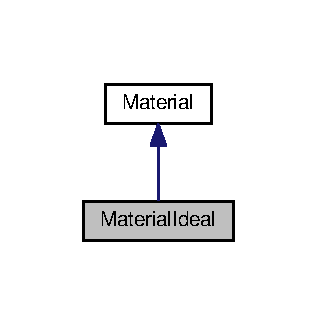
\includegraphics[width=152pt]{classMaterialIdeal__inherit__graph}
\end{center}
\end{figure}


Collaboration diagram for Material\+Ideal\+:
\nopagebreak
\begin{figure}[H]
\begin{center}
\leavevmode
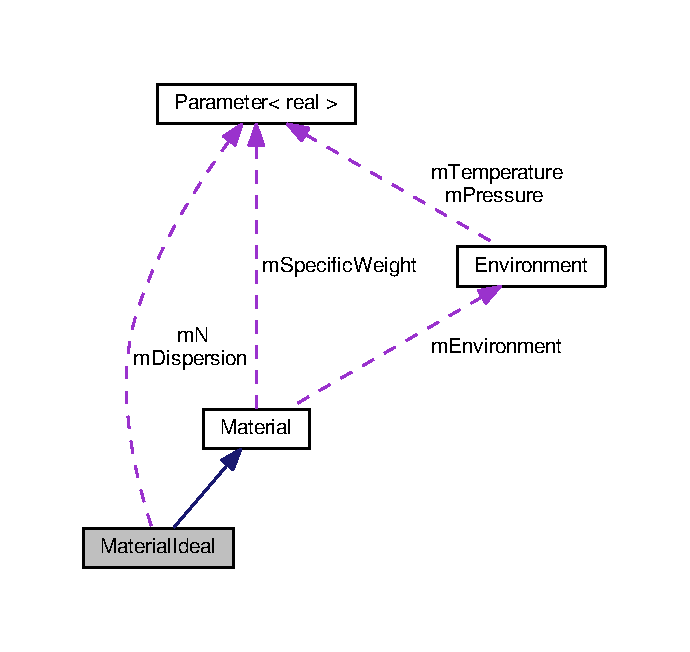
\includegraphics[width=331pt]{classMaterialIdeal__coll__graph}
\end{center}
\end{figure}
\subsection*{Public Member Functions}
\begin{DoxyCompactItemize}
\item 
\hyperlink{classMaterialIdeal_a81f6c27aef2251e7d810fa4d9521d9e4}{Material\+Ideal} (std\+::string name, \hyperlink{classEnvironment}{Environment} $\ast$env, real n, real dispersion=0, real absorption=0)
\begin{DoxyCompactList}\small\item\em ctor \end{DoxyCompactList}\item 
virtual real \hyperlink{classMaterialIdeal_a21833d3f466424ee62ee70e02de1ee49}{get\+Refractive\+Index} (real wavelength, std\+::complex$<$ real $>$ ex, std\+::complex$<$ real $>$ ey, std\+::complex$<$ real $>$ ez)
\end{DoxyCompactItemize}
\subsection*{Protected Attributes}
\begin{DoxyCompactItemize}
\item 
\hyperlink{classParameter}{Parameter}$<$ real $>$ \hyperlink{classMaterialIdeal_aa2a06bb4e433a2c039714e85f5e777c1}{mN}\hypertarget{classMaterialIdeal_aa2a06bb4e433a2c039714e85f5e777c1}{}\label{classMaterialIdeal_aa2a06bb4e433a2c039714e85f5e777c1}

\begin{DoxyCompactList}\small\item\em refractive index \end{DoxyCompactList}\item 
\hyperlink{classParameter}{Parameter}$<$ real $>$ \hyperlink{classMaterialIdeal_a1e1974c42234bddf7c7e2ba52cf316a0}{m\+Dispersion}\hypertarget{classMaterialIdeal_a1e1974c42234bddf7c7e2ba52cf316a0}{}\label{classMaterialIdeal_a1e1974c42234bddf7c7e2ba52cf316a0}

\begin{DoxyCompactList}\small\item\em Dispersion. \end{DoxyCompactList}\end{DoxyCompactItemize}


\subsection{Detailed Description}
\hyperlink{classMaterialIdeal}{Material\+Ideal} represents all ideal Materials. 

Subclasses have to derived

In the future we will derive classes (e.\+g. metamaterials) from this class. However\+: We have to deeply think about the interface then !

Refractive Index and Reflection -\/ Wavelength
\begin{DoxyItemize}
\item Polarization
\item Orientation of \hyperlink{classMaterial}{Material}
\end{DoxyItemize}

We also need Subclasses for
\begin{DoxyItemize}
\item \hyperlink{classMaterialIdeal}{Material\+Ideal} (perfect mirrors, Glass with given refractive index etc..)
\item Materials that need different equations for different spectral regimes
\end{DoxyItemize}

in General\+: we should have a look at optical material in General to get the right (very general) interface 

\subsection{Constructor \& Destructor Documentation}
\index{Material\+Ideal@{Material\+Ideal}!Material\+Ideal@{Material\+Ideal}}
\index{Material\+Ideal@{Material\+Ideal}!Material\+Ideal@{Material\+Ideal}}
\subsubsection[{\texorpdfstring{Material\+Ideal(std\+::string name, Environment $\ast$env, real n, real dispersion=0, real absorption=0)}{MaterialIdeal(std::string name, Environment *env, real n, real dispersion=0, real absorption=0)}}]{\setlength{\rightskip}{0pt plus 5cm}Material\+Ideal\+::\+Material\+Ideal (
\begin{DoxyParamCaption}
\item[{std\+::string}]{name, }
\item[{{\bf Environment} $\ast$}]{env, }
\item[{real}]{n, }
\item[{real}]{dispersion = {\ttfamily 0}, }
\item[{real}]{absorption = {\ttfamily 0}}
\end{DoxyParamCaption}
)}\hypertarget{classMaterialIdeal_a81f6c27aef2251e7d810fa4d9521d9e4}{}\label{classMaterialIdeal_a81f6c27aef2251e7d810fa4d9521d9e4}


ctor 


\begin{DoxyParams}{Parameters}
{\em n} & refractive index \\
\hline
\end{DoxyParams}


\subsection{Member Function Documentation}
\index{Material\+Ideal@{Material\+Ideal}!get\+Refractive\+Index@{get\+Refractive\+Index}}
\index{get\+Refractive\+Index@{get\+Refractive\+Index}!Material\+Ideal@{Material\+Ideal}}
\subsubsection[{\texorpdfstring{get\+Refractive\+Index(real wavelength, std\+::complex$<$ real $>$ ex, std\+::complex$<$ real $>$ ey, std\+::complex$<$ real $>$ ez)}{getRefractiveIndex(real wavelength, std::complex< real > ex, std::complex< real > ey, std::complex< real > ez)}}]{\setlength{\rightskip}{0pt plus 5cm}real Material\+Ideal\+::get\+Refractive\+Index (
\begin{DoxyParamCaption}
\item[{real}]{wavelength, }
\item[{std\+::complex$<$ real $>$}]{ex, }
\item[{std\+::complex$<$ real $>$}]{ey, }
\item[{std\+::complex$<$ real $>$}]{ez}
\end{DoxyParamCaption}
)\hspace{0.3cm}{\ttfamily [virtual]}}\hypertarget{classMaterialIdeal_a21833d3f466424ee62ee70e02de1ee49}{}\label{classMaterialIdeal_a21833d3f466424ee62ee70e02de1ee49}

\begin{DoxyParams}{Parameters}
{\em wavelength} & wavelength in m \\
\hline
{\em ex} & polarization electrical field in x direction in global coordinates \\
\hline
{\em ey} & polarization electrical field in x direction in global coordinates \\
\hline
{\em ez} & polarization electrical field in x direction in global coordinates \\
\hline
\end{DoxyParams}


Implements \hyperlink{classMaterial_a8994560db37896679e16161a7a7cb75b}{Material}.



The documentation for this class was generated from the following files\+:\begin{DoxyCompactItemize}
\item 
\hyperlink{materialideal_8h}{materialideal.\+h}\item 
materialideal.\+cc\end{DoxyCompactItemize}

\hypertarget{classOpticalSystem}{}\section{Optical\+System Class Reference}
\label{classOpticalSystem}\index{Optical\+System@{Optical\+System}}


Describes the complete optical system.  




{\ttfamily \#include $<$opticalsystem.\+h$>$}



Collaboration diagram for Optical\+System\+:
\nopagebreak
\begin{figure}[H]
\begin{center}
\leavevmode
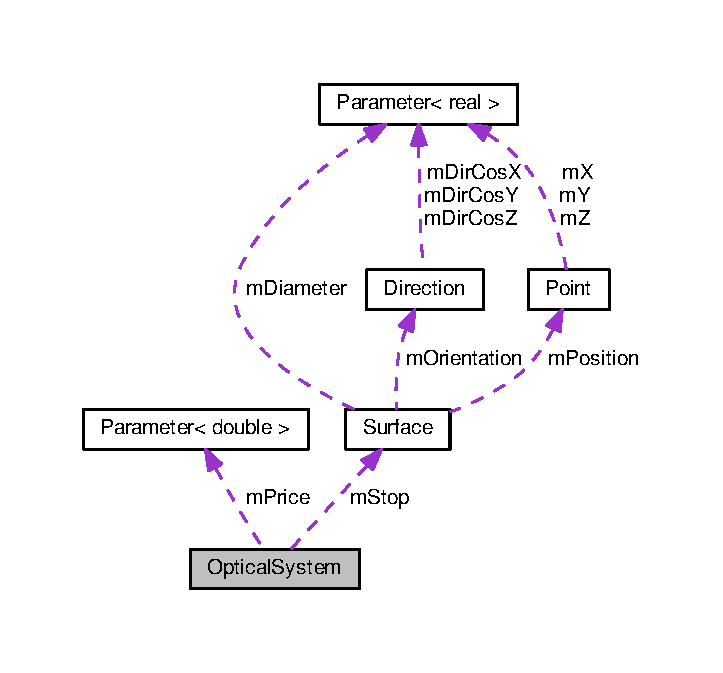
\includegraphics[width=347pt]{classOpticalSystem__coll__graph}
\end{center}
\end{figure}
\subsection*{Public Member Functions}
\begin{DoxyCompactItemize}
\item 
void \hyperlink{classOpticalSystem_a9ea225f3366e3f6794985173be3f42ba}{add\+Element} (\hyperlink{classElement}{Element} $\ast$const e)
\begin{DoxyCompactList}\small\item\em add one \hyperlink{classElement}{Element} at the end of the system \end{DoxyCompactList}\item 
int \hyperlink{classOpticalSystem_a097a1fe0bbddacebab645c5f0dc09361}{set\+Element} (\hyperlink{classElement}{Element} $\ast$const e, int nr)
\begin{DoxyCompactList}\small\item\em replace \hyperlink{classElement}{Element} number n \end{DoxyCompactList}\item 
\hyperlink{classElement}{Element} $\ast$const \hyperlink{classOpticalSystem_a66d8de4ccd5ae4301db88f232f435081}{get\+Element} (int nr) const 
\begin{DoxyCompactList}\small\item\em set the \hyperlink{classElement}{Element} number n \end{DoxyCompactList}\end{DoxyCompactItemize}
\subsection*{Protected Attributes}
\begin{DoxyCompactItemize}
\item 
std\+::vector$<$ \hyperlink{classElement}{Element} $\ast$ $>$ \hyperlink{classOpticalSystem_a631ce48d96804db9cffcc0820bd58c09}{m\+Elements}\hypertarget{classOpticalSystem_a631ce48d96804db9cffcc0820bd58c09}{}\label{classOpticalSystem_a631ce48d96804db9cffcc0820bd58c09}

\begin{DoxyCompactList}\small\item\em Here, the elements are stored. \end{DoxyCompactList}\item 
\hyperlink{classParameter}{Parameter}$<$ double $>$ \hyperlink{classOpticalSystem_ae27cdbd3c25a95204813bc0f8da69bd3}{m\+Price}\hypertarget{classOpticalSystem_ae27cdbd3c25a95204813bc0f8da69bd3}{}\label{classOpticalSystem_ae27cdbd3c25a95204813bc0f8da69bd3}

\begin{DoxyCompactList}\small\item\em Price of the optical system. \end{DoxyCompactList}\item 
\hyperlink{classSurface}{Surface} $\ast$ \hyperlink{classOpticalSystem_a98b21335a43785df339f04c7e05100d5}{m\+Stop}\hypertarget{classOpticalSystem_a98b21335a43785df339f04c7e05100d5}{}\label{classOpticalSystem_a98b21335a43785df339f04c7e05100d5}

\begin{DoxyCompactList}\small\item\em for classic optical design we need a stop S\+U\+R\+F\+A\+CE \end{DoxyCompactList}\end{DoxyCompactItemize}


\subsection{Detailed Description}
Describes the complete optical system. 

We trace light through optical systems. During the trace different components are encountered by the light. These things are handled in the propagation and interaction classes. However, the hardware of the whole optical system (consisting of lenses, surfaces, materials etc. is stored and managed in this class (and the important subclass \hyperlink{classElement}{Element}).

Mainly the optical system consists of Elements (and additional information) And of course, Elements consist of Surfaces, Materials, Coatings etc.

The class never creates or destructs elements (or surfaces) (otherwise we would have to use smartpointer or something similar)

\begin{DoxyDate}{Date}
07.\+4.\+2017 
\end{DoxyDate}
\begin{DoxyAuthor}{Author}
Tobias Haist (\href{mailto:haist@ito.uni-stuttgart.de}{\tt haist@ito.\+uni-\/stuttgart.\+de}) 
\end{DoxyAuthor}


\subsection{Member Function Documentation}
\index{Optical\+System@{Optical\+System}!add\+Element@{add\+Element}}
\index{add\+Element@{add\+Element}!Optical\+System@{Optical\+System}}
\subsubsection[{\texorpdfstring{add\+Element(\+Element $\ast$const e)}{addElement(Element *const e)}}]{\setlength{\rightskip}{0pt plus 5cm}void Optical\+System\+::add\+Element (
\begin{DoxyParamCaption}
\item[{{\bf Element} $\ast$const}]{e}
\end{DoxyParamCaption}
)}\hypertarget{classOpticalSystem_a9ea225f3366e3f6794985173be3f42ba}{}\label{classOpticalSystem_a9ea225f3366e3f6794985173be3f42ba}


add one \hyperlink{classElement}{Element} at the end of the system 


\begin{DoxyParams}{Parameters}
{\em e} & Pointer to \hyperlink{classElement}{Element} to be added to end of list \\
\hline
\end{DoxyParams}
\index{Optical\+System@{Optical\+System}!get\+Element@{get\+Element}}
\index{get\+Element@{get\+Element}!Optical\+System@{Optical\+System}}
\subsubsection[{\texorpdfstring{get\+Element(int nr) const }{getElement(int nr) const }}]{\setlength{\rightskip}{0pt plus 5cm}{\bf Element} $\ast$const Optical\+System\+::get\+Element (
\begin{DoxyParamCaption}
\item[{int}]{nr}
\end{DoxyParamCaption}
) const}\hypertarget{classOpticalSystem_a66d8de4ccd5ae4301db88f232f435081}{}\label{classOpticalSystem_a66d8de4ccd5ae4301db88f232f435081}


set the \hyperlink{classElement}{Element} number n 


\begin{DoxyParams}{Parameters}
{\em nr} & index (0 ... size) of element of the optical system \\
\hline
\end{DoxyParams}
\begin{DoxyReturn}{Returns}
Pointer to \hyperlink{classElement}{Element} number nr 
\end{DoxyReturn}
\index{Optical\+System@{Optical\+System}!set\+Element@{set\+Element}}
\index{set\+Element@{set\+Element}!Optical\+System@{Optical\+System}}
\subsubsection[{\texorpdfstring{set\+Element(\+Element $\ast$const e, int nr)}{setElement(Element *const e, int nr)}}]{\setlength{\rightskip}{0pt plus 5cm}int Optical\+System\+::set\+Element (
\begin{DoxyParamCaption}
\item[{{\bf Element} $\ast$const}]{e, }
\item[{int}]{nr}
\end{DoxyParamCaption}
)}\hypertarget{classOpticalSystem_a097a1fe0bbddacebab645c5f0dc09361}{}\label{classOpticalSystem_a097a1fe0bbddacebab645c5f0dc09361}


replace \hyperlink{classElement}{Element} number n 


\begin{DoxyParams}{Parameters}
{\em nr} & index (0 ... size) of element of the optical system \\
\hline
{\em Pointer} & to \hyperlink{classElement}{Element} number nr \\
\hline
\end{DoxyParams}
\begin{DoxyReturn}{Returns}
-\/1 if index is out of bounds, otherwise\+: nr 
\end{DoxyReturn}


The documentation for this class was generated from the following files\+:\begin{DoxyCompactItemize}
\item 
\hyperlink{opticalsystem_8h}{opticalsystem.\+h}\item 
\hyperlink{opticalsystem_8cc}{opticalsystem.\+cc}\end{DoxyCompactItemize}

\hypertarget{classParameter}{}\section{Parameter$<$ Type $>$ Class Template Reference}
\label{classParameter}\index{Parameter$<$ Type $>$@{Parameter$<$ Type $>$}}


\hyperlink{classParameter}{Parameter} manages changeable Parameters (e.\+g. for optimization)  




{\ttfamily \#include $<$parameter.\+h$>$}



Collaboration diagram for Parameter$<$ Type $>$\+:\nopagebreak
\begin{figure}[H]
\begin{center}
\leavevmode
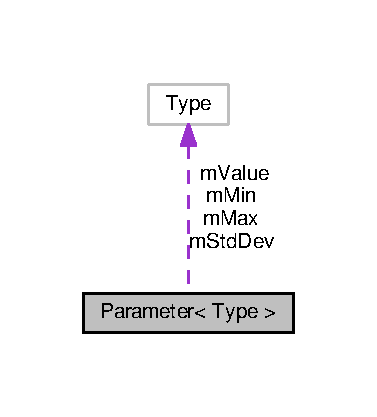
\includegraphics[width=181pt]{classParameter__coll__graph}
\end{center}
\end{figure}
\subsection*{Public Member Functions}
\begin{DoxyCompactItemize}
\item 
\hyperlink{classParameter_a6000e8cd47acceb8748300e8c82657a3}{Parameter} ()\hypertarget{classParameter_a6000e8cd47acceb8748300e8c82657a3}{}\label{classParameter_a6000e8cd47acceb8748300e8c82657a3}

\begin{DoxyCompactList}\small\item\em std ctor \end{DoxyCompactList}\item 
\hyperlink{classParameter_a55f791445b9a159d7b5f1ce0b4f786b9}{Parameter} (Type x)
\begin{DoxyCompactList}\small\item\em construction with global coordinates \end{DoxyCompactList}\item 
void \hyperlink{classParameter_a9013b47b1190dbb977df02dcf5101d6d}{set\+Value} (Type x)
\begin{DoxyCompactList}\small\item\em set Value to x \end{DoxyCompactList}\item 
Type \hyperlink{classParameter_ac20cb89fbbc4cb6dfdc9779a473659b8}{get\+Value} () const 
\begin{DoxyCompactList}\small\item\em get the Value \end{DoxyCompactList}\item 
void \hyperlink{classParameter_af4017adaebcb220cfcb046bfc9f2005b}{set\+Minimum} (Type x)
\begin{DoxyCompactList}\small\item\em set the minimum value to x \end{DoxyCompactList}\item 
Type \hyperlink{classParameter_a47b69ec50b78a9202ba470ec79282f2b}{get\+Minimum} () const 
\begin{DoxyCompactList}\small\item\em get the minimum Value \end{DoxyCompactList}\item 
void \hyperlink{classParameter_a9148818a721c6b20e25aaa981c932974}{set\+Maximum} (Type x)
\begin{DoxyCompactList}\small\item\em set the maximum value to x \end{DoxyCompactList}\item 
Type \hyperlink{classParameter_a4bff89ddd1c3a3e8ebac73c907cb432e}{get\+Maximum} () const 
\begin{DoxyCompactList}\small\item\em get the maximum Value \end{DoxyCompactList}\item 
void \hyperlink{classParameter_a85ecc82055bbb4e7724d82ccff6bf3b6}{set\+Std\+Dev} (Type x)
\begin{DoxyCompactList}\small\item\em set the standard deviation of Value \end{DoxyCompactList}\item 
Type \hyperlink{classParameter_a01d2bff5f7ad0d99a3bf3a907421ffee}{get\+Std\+Dev} () const 
\begin{DoxyCompactList}\small\item\em get the standard deviation of Value \end{DoxyCompactList}\item 
void \hyperlink{classParameter_a4030a197e21b6f2a968047b6da958138}{set\+Modifier} (type\+Modifier x)
\begin{DoxyCompactList}\small\item\em set the modifier \end{DoxyCompactList}\item 
type\+Modifier \hyperlink{classParameter_aa6f79e36bd16f49c33302181fe5131d8}{get\+Modifier} () const 
\begin{DoxyCompactList}\small\item\em get the modifier \end{DoxyCompactList}\end{DoxyCompactItemize}
\subsection*{Protected Attributes}
\begin{DoxyCompactItemize}
\item 
Type \hyperlink{classParameter_a631a80711abe692a1ce7af67abc0a097}{m\+Value}\hypertarget{classParameter_a631a80711abe692a1ce7af67abc0a097}{}\label{classParameter_a631a80711abe692a1ce7af67abc0a097}

\begin{DoxyCompactList}\small\item\em (mean) value of parameter \end{DoxyCompactList}\item 
Type \hyperlink{classParameter_a725584b7a8af84b3e5f811b27b12615f}{m\+Min}\hypertarget{classParameter_a725584b7a8af84b3e5f811b27b12615f}{}\label{classParameter_a725584b7a8af84b3e5f811b27b12615f}

\begin{DoxyCompactList}\small\item\em minimum allowed value of paramter \end{DoxyCompactList}\item 
Type \hyperlink{classParameter_a67920b1bd3610cc8fcb43f1811d31e4b}{m\+Max}\hypertarget{classParameter_a67920b1bd3610cc8fcb43f1811d31e4b}{}\label{classParameter_a67920b1bd3610cc8fcb43f1811d31e4b}

\begin{DoxyCompactList}\small\item\em maximum allowed value of paramter \end{DoxyCompactList}\item 
Type \hyperlink{classParameter_a23b648958657c9949667af624bcac95b}{m\+Std\+Dev}\hypertarget{classParameter_a23b648958657c9949667af624bcac95b}{}\label{classParameter_a23b648958657c9949667af624bcac95b}

\begin{DoxyCompactList}\small\item\em standard deviation of parameter (for tolerancing) \end{DoxyCompactList}\item 
type\+Modifier \hyperlink{classParameter_a8e555cfec6a44778d4d04a81831c445e}{m\+Modifier}\hypertarget{classParameter_a8e555cfec6a44778d4d04a81831c445e}{}\label{classParameter_a8e555cfec6a44778d4d04a81831c445e}

\begin{DoxyCompactList}\small\item\em is this a variable or fixed or pickup \end{DoxyCompactList}\end{DoxyCompactItemize}


\subsection{Detailed Description}
\subsubsection*{template$<$class Type$>$\\*
class Parameter$<$ Type $>$}

\hyperlink{classParameter}{Parameter} manages changeable Parameters (e.\+g. for optimization) 

The template class stores the actual or mean value together with the allowed variation (given as a standard deviation) and allowed minimum and maximum value. This is used e.\+g. for tolerancing and optimization

The parameters minimum, maximum, std\+Dev in principle only make sense for numerical parameters. However, we also will have the case that parameters can vary based on some discrete values (e.\+g. internal index number in glass catalog) out of a list of certain parameters. the main application is responsible to make the translation in this case from integer values to certain usable parameters. (If this is necessary at not only a few places in the code, we might add in the future an additional helper class to handle this translation)

class should be instantiated for real(double), int, string

\begin{DoxyDate}{Date}
07.\+4.\+2017 
\end{DoxyDate}
\begin{DoxyAuthor}{Author}
Tobias Haist (\href{mailto:haist@ito.uni-stuttgart.de}{\tt haist@ito.\+uni-\/stuttgart.\+de}) 
\end{DoxyAuthor}


\subsection{Constructor \& Destructor Documentation}
\index{Parameter@{Parameter}!Parameter@{Parameter}}
\index{Parameter@{Parameter}!Parameter@{Parameter}}
\subsubsection[{\texorpdfstring{Parameter(\+Type x)}{Parameter(Type x)}}]{\setlength{\rightskip}{0pt plus 5cm}template$<$class Type$>$ {\bf Parameter}$<$ Type $>$\+::{\bf Parameter} (
\begin{DoxyParamCaption}
\item[{Type}]{x}
\end{DoxyParamCaption}
)}\hypertarget{classParameter_a55f791445b9a159d7b5f1ce0b4f786b9}{}\label{classParameter_a55f791445b9a159d7b5f1ce0b4f786b9}


construction with global coordinates 


\begin{DoxyParams}{Parameters}
{\em a} & Value to be set \\
\hline
\end{DoxyParams}


\subsection{Member Function Documentation}
\index{Parameter@{Parameter}!get\+Maximum@{get\+Maximum}}
\index{get\+Maximum@{get\+Maximum}!Parameter@{Parameter}}
\subsubsection[{\texorpdfstring{get\+Maximum() const }{getMaximum() const }}]{\setlength{\rightskip}{0pt plus 5cm}template$<$class Type $>$ Type {\bf Parameter}$<$ Type $>$\+::get\+Maximum (
\begin{DoxyParamCaption}
{}
\end{DoxyParamCaption}
) const}\hypertarget{classParameter_a4bff89ddd1c3a3e8ebac73c907cb432e}{}\label{classParameter_a4bff89ddd1c3a3e8ebac73c907cb432e}


get the maximum Value 

\begin{DoxyReturn}{Returns}
current Value 
\end{DoxyReturn}
\index{Parameter@{Parameter}!get\+Minimum@{get\+Minimum}}
\index{get\+Minimum@{get\+Minimum}!Parameter@{Parameter}}
\subsubsection[{\texorpdfstring{get\+Minimum() const }{getMinimum() const }}]{\setlength{\rightskip}{0pt plus 5cm}template$<$class Type $>$ Type {\bf Parameter}$<$ Type $>$\+::get\+Minimum (
\begin{DoxyParamCaption}
{}
\end{DoxyParamCaption}
) const}\hypertarget{classParameter_a47b69ec50b78a9202ba470ec79282f2b}{}\label{classParameter_a47b69ec50b78a9202ba470ec79282f2b}


get the minimum Value 

\begin{DoxyReturn}{Returns}
current Value 
\end{DoxyReturn}
\index{Parameter@{Parameter}!get\+Modifier@{get\+Modifier}}
\index{get\+Modifier@{get\+Modifier}!Parameter@{Parameter}}
\subsubsection[{\texorpdfstring{get\+Modifier() const }{getModifier() const }}]{\setlength{\rightskip}{0pt plus 5cm}template$<$class Type $>$ type\+Modifier {\bf Parameter}$<$ Type $>$\+::get\+Modifier (
\begin{DoxyParamCaption}
{}
\end{DoxyParamCaption}
) const}\hypertarget{classParameter_aa6f79e36bd16f49c33302181fe5131d8}{}\label{classParameter_aa6f79e36bd16f49c33302181fe5131d8}


get the modifier 

\begin{DoxyReturn}{Returns}
current Value 
\end{DoxyReturn}
\index{Parameter@{Parameter}!get\+Std\+Dev@{get\+Std\+Dev}}
\index{get\+Std\+Dev@{get\+Std\+Dev}!Parameter@{Parameter}}
\subsubsection[{\texorpdfstring{get\+Std\+Dev() const }{getStdDev() const }}]{\setlength{\rightskip}{0pt plus 5cm}template$<$class Type $>$ Type {\bf Parameter}$<$ Type $>$\+::get\+Std\+Dev (
\begin{DoxyParamCaption}
{}
\end{DoxyParamCaption}
) const}\hypertarget{classParameter_a01d2bff5f7ad0d99a3bf3a907421ffee}{}\label{classParameter_a01d2bff5f7ad0d99a3bf3a907421ffee}


get the standard deviation of Value 

\begin{DoxyReturn}{Returns}
current Value 
\end{DoxyReturn}
\index{Parameter@{Parameter}!get\+Value@{get\+Value}}
\index{get\+Value@{get\+Value}!Parameter@{Parameter}}
\subsubsection[{\texorpdfstring{get\+Value() const }{getValue() const }}]{\setlength{\rightskip}{0pt plus 5cm}template$<$class Type $>$ Type {\bf Parameter}$<$ Type $>$\+::get\+Value (
\begin{DoxyParamCaption}
{}
\end{DoxyParamCaption}
) const}\hypertarget{classParameter_ac20cb89fbbc4cb6dfdc9779a473659b8}{}\label{classParameter_ac20cb89fbbc4cb6dfdc9779a473659b8}


get the Value 

\begin{DoxyReturn}{Returns}
current Value 
\end{DoxyReturn}
\index{Parameter@{Parameter}!set\+Maximum@{set\+Maximum}}
\index{set\+Maximum@{set\+Maximum}!Parameter@{Parameter}}
\subsubsection[{\texorpdfstring{set\+Maximum(\+Type x)}{setMaximum(Type x)}}]{\setlength{\rightskip}{0pt plus 5cm}template$<$class Type$>$ void {\bf Parameter}$<$ Type $>$\+::set\+Maximum (
\begin{DoxyParamCaption}
\item[{Type}]{x}
\end{DoxyParamCaption}
)}\hypertarget{classParameter_a9148818a721c6b20e25aaa981c932974}{}\label{classParameter_a9148818a721c6b20e25aaa981c932974}


set the maximum value to x 


\begin{DoxyParams}{Parameters}
{\em a} & Value to be set \\
\hline
\end{DoxyParams}
\index{Parameter@{Parameter}!set\+Minimum@{set\+Minimum}}
\index{set\+Minimum@{set\+Minimum}!Parameter@{Parameter}}
\subsubsection[{\texorpdfstring{set\+Minimum(\+Type x)}{setMinimum(Type x)}}]{\setlength{\rightskip}{0pt plus 5cm}template$<$class Type$>$ void {\bf Parameter}$<$ Type $>$\+::set\+Minimum (
\begin{DoxyParamCaption}
\item[{Type}]{x}
\end{DoxyParamCaption}
)}\hypertarget{classParameter_af4017adaebcb220cfcb046bfc9f2005b}{}\label{classParameter_af4017adaebcb220cfcb046bfc9f2005b}


set the minimum value to x 


\begin{DoxyParams}{Parameters}
{\em a} & Value to be set \\
\hline
\end{DoxyParams}
\index{Parameter@{Parameter}!set\+Modifier@{set\+Modifier}}
\index{set\+Modifier@{set\+Modifier}!Parameter@{Parameter}}
\subsubsection[{\texorpdfstring{set\+Modifier(type\+Modifier x)}{setModifier(typeModifier x)}}]{\setlength{\rightskip}{0pt plus 5cm}template$<$class Type $>$ void {\bf Parameter}$<$ Type $>$\+::set\+Modifier (
\begin{DoxyParamCaption}
\item[{type\+Modifier}]{x}
\end{DoxyParamCaption}
)}\hypertarget{classParameter_a4030a197e21b6f2a968047b6da958138}{}\label{classParameter_a4030a197e21b6f2a968047b6da958138}


set the modifier 


\begin{DoxyParams}{Parameters}
{\em a} & Value to be set \\
\hline
\end{DoxyParams}
\index{Parameter@{Parameter}!set\+Std\+Dev@{set\+Std\+Dev}}
\index{set\+Std\+Dev@{set\+Std\+Dev}!Parameter@{Parameter}}
\subsubsection[{\texorpdfstring{set\+Std\+Dev(\+Type x)}{setStdDev(Type x)}}]{\setlength{\rightskip}{0pt plus 5cm}template$<$class Type$>$ void {\bf Parameter}$<$ Type $>$\+::set\+Std\+Dev (
\begin{DoxyParamCaption}
\item[{Type}]{x}
\end{DoxyParamCaption}
)}\hypertarget{classParameter_a85ecc82055bbb4e7724d82ccff6bf3b6}{}\label{classParameter_a85ecc82055bbb4e7724d82ccff6bf3b6}


set the standard deviation of Value 


\begin{DoxyParams}{Parameters}
{\em a} & Value to be set \\
\hline
\end{DoxyParams}
\index{Parameter@{Parameter}!set\+Value@{set\+Value}}
\index{set\+Value@{set\+Value}!Parameter@{Parameter}}
\subsubsection[{\texorpdfstring{set\+Value(\+Type x)}{setValue(Type x)}}]{\setlength{\rightskip}{0pt plus 5cm}template$<$class Type$>$ void {\bf Parameter}$<$ Type $>$\+::set\+Value (
\begin{DoxyParamCaption}
\item[{Type}]{x}
\end{DoxyParamCaption}
)}\hypertarget{classParameter_a9013b47b1190dbb977df02dcf5101d6d}{}\label{classParameter_a9013b47b1190dbb977df02dcf5101d6d}


set Value to x 


\begin{DoxyParams}{Parameters}
{\em a} & Value to be set \\
\hline
\end{DoxyParams}


The documentation for this class was generated from the following files\+:\begin{DoxyCompactItemize}
\item 
\hyperlink{parameter_8h}{parameter.\+h}\item 
parameter.\+cc\end{DoxyCompactItemize}

\hypertarget{classPoint}{}\section{Point Class Reference}
\label{classPoint}\index{Point@{Point}}


\hyperlink{classPoint}{Point} manages Points/\+Positions in Space.  




{\ttfamily \#include $<$point.\+h$>$}



Collaboration diagram for Point\+:
\nopagebreak
\begin{figure}[H]
\begin{center}
\leavevmode
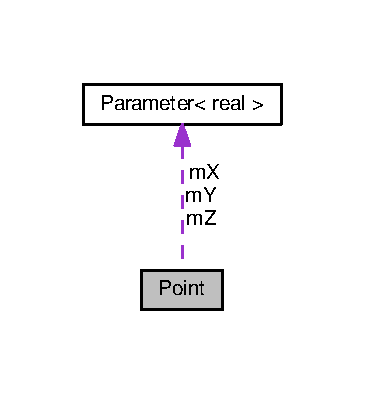
\includegraphics[width=175pt]{classPoint__coll__graph}
\end{center}
\end{figure}
\subsection*{Public Member Functions}
\begin{DoxyCompactItemize}
\item 
\hyperlink{classPoint_af73f855d0ef3a5f76c63ffc014d28bec}{Point} (real x=0, real y=0, real z=0)
\begin{DoxyCompactList}\small\item\em construction with global coordinates \end{DoxyCompactList}\end{DoxyCompactItemize}
\subsection*{Protected Attributes}
\begin{DoxyCompactItemize}
\item 
\hyperlink{classParameter}{Parameter}$<$ real $>$ \hyperlink{classPoint_acbee7418f6236b827d9dccd1d37b39fb}{mX}\hypertarget{classPoint_acbee7418f6236b827d9dccd1d37b39fb}{}\label{classPoint_acbee7418f6236b827d9dccd1d37b39fb}

\begin{DoxyCompactList}\small\item\em x coordinate in global coordinate system \end{DoxyCompactList}\item 
\hyperlink{classParameter}{Parameter}$<$ real $>$ \hyperlink{classPoint_a3503cea70b25f3746ff4e3e9282248a0}{mY}\hypertarget{classPoint_a3503cea70b25f3746ff4e3e9282248a0}{}\label{classPoint_a3503cea70b25f3746ff4e3e9282248a0}

\begin{DoxyCompactList}\small\item\em y coordinate in global coordinate system \end{DoxyCompactList}\item 
\hyperlink{classParameter}{Parameter}$<$ real $>$ \hyperlink{classPoint_a55932304ba34c80cf489a3b374dab965}{mZ}\hypertarget{classPoint_a55932304ba34c80cf489a3b374dab965}{}\label{classPoint_a55932304ba34c80cf489a3b374dab965}

\begin{DoxyCompactList}\small\item\em z coordinate in global coordinate system \end{DoxyCompactList}\end{DoxyCompactItemize}


\subsection{Detailed Description}
\hyperlink{classPoint}{Point} manages Points/\+Positions in Space. 

This is the basic class for representing the position of a point. The point can be given, of course, in different coordinate systems. However, it is stored in \char`\"{}the\char`\"{} one and only global coordinate system. Methods for obtaining the position in other systems are given.

\begin{DoxyDate}{Date}
07.\+4.\+2017 
\end{DoxyDate}
\begin{DoxyAuthor}{Author}
Tobias Haist (\href{mailto:haist@ito.uni-stuttgart.de}{\tt haist@ito.\+uni-\/stuttgart.\+de}) 
\end{DoxyAuthor}


\subsection{Constructor \& Destructor Documentation}
\index{Point@{Point}!Point@{Point}}
\index{Point@{Point}!Point@{Point}}
\subsubsection[{\texorpdfstring{Point(real x=0, real y=0, real z=0)}{Point(real x=0, real y=0, real z=0)}}]{\setlength{\rightskip}{0pt plus 5cm}Point\+::\+Point (
\begin{DoxyParamCaption}
\item[{real}]{x = {\ttfamily 0}, }
\item[{real}]{y = {\ttfamily 0}, }
\item[{real}]{z = {\ttfamily 0}}
\end{DoxyParamCaption}
)}\hypertarget{classPoint_af73f855d0ef3a5f76c63ffc014d28bec}{}\label{classPoint_af73f855d0ef3a5f76c63ffc014d28bec}


construction with global coordinates 


\begin{DoxyParams}{Parameters}
{\em x} & global x coordinate of point \\
\hline
{\em y} & global y coordinate of point \\
\hline
{\em z} & global z coordinate of point \\
\hline
\end{DoxyParams}


The documentation for this class was generated from the following files\+:\begin{DoxyCompactItemize}
\item 
\hyperlink{point_8h}{point.\+h}\item 
\hyperlink{point_8cc}{point.\+cc}\end{DoxyCompactItemize}

\hypertarget{classRay}{}\section{Ray Class Reference}
\label{classRay}\index{Ray@{Ray}}


\hyperlink{classRay}{Ray} manages optical (polarized or unpolarized) Rays.  




{\ttfamily \#include $<$ray.\+h$>$}



Inheritance diagram for Ray\+:\nopagebreak
\begin{figure}[H]
\begin{center}
\leavevmode
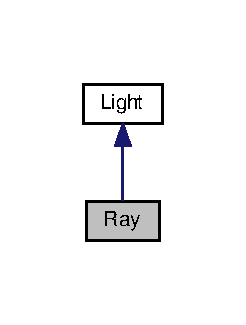
\includegraphics[width=118pt]{classRay__inherit__graph}
\end{center}
\end{figure}


Collaboration diagram for Ray\+:
\nopagebreak
\begin{figure}[H]
\begin{center}
\leavevmode
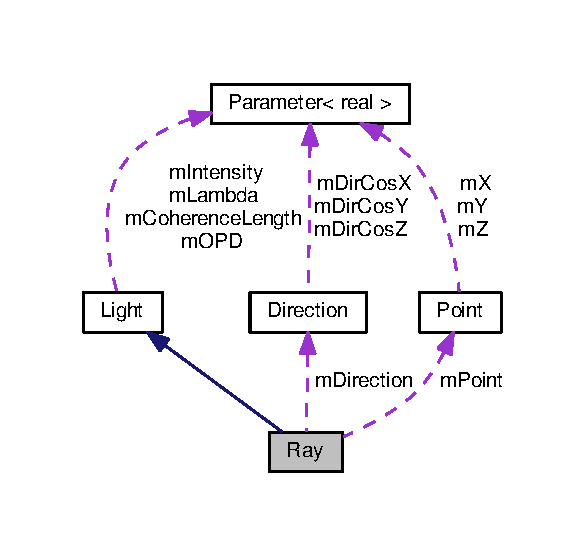
\includegraphics[width=282pt]{classRay__coll__graph}
\end{center}
\end{figure}
\subsection*{Public Member Functions}
\begin{DoxyCompactItemize}
\item 
\hyperlink{classRay_abe7c9d6bfd243e256a5a69f5ab9ade39}{Ray} (real lambda=500e-\/9, real intensity=1)
\begin{DoxyCompactList}\small\item\em ctor \end{DoxyCompactList}\item 
\hyperlink{classRay_a248f18e16b380a3518608f23c7f3f82f}{Ray} (real lambda, real intensity, \hyperlink{classPoint}{Point} $\ast$const p, \hyperlink{classDirection}{Direction} $\ast$const dir)
\begin{DoxyCompactList}\small\item\em construction with global coordinates \end{DoxyCompactList}\end{DoxyCompactItemize}
\subsection*{Protected Attributes}
\begin{DoxyCompactItemize}
\item 
\hyperlink{classPoint}{Point} \hyperlink{classRay_a9665b2e2fccaffdcc4c7b682d578153b}{m\+Point}\hypertarget{classRay_a9665b2e2fccaffdcc4c7b682d578153b}{}\label{classRay_a9665b2e2fccaffdcc4c7b682d578153b}

\begin{DoxyCompactList}\small\item\em start point \end{DoxyCompactList}\item 
\hyperlink{classDirection}{Direction} \hyperlink{classRay_aebcf4d0d29d676055973101739e2261b}{m\+Direction}\hypertarget{classRay_aebcf4d0d29d676055973101739e2261b}{}\label{classRay_aebcf4d0d29d676055973101739e2261b}

\begin{DoxyCompactList}\small\item\em \hyperlink{classDirection}{Direction} cosines. \end{DoxyCompactList}\end{DoxyCompactItemize}


\subsection{Detailed Description}
\hyperlink{classRay}{Ray} manages optical (polarized or unpolarized) Rays. 

This is the basic class for representing light in the geometrical model. The concept of the ray is an idealized one. The ray has zero extension and divergence. Our ray is polarized (Jones Vector) or unpolarized, has one specific wavelength and energy.

\begin{DoxyDate}{Date}
07.\+4.\+2017 
\end{DoxyDate}
\begin{DoxyAuthor}{Author}
Tobias Haist (\href{mailto:haist@ito.uni-stuttgart.de}{\tt haist@ito.\+uni-\/stuttgart.\+de}) 
\end{DoxyAuthor}


\subsection{Constructor \& Destructor Documentation}
\index{Ray@{Ray}!Ray@{Ray}}
\index{Ray@{Ray}!Ray@{Ray}}
\subsubsection[{\texorpdfstring{Ray(real lambda=500e-\/9, real intensity=1)}{Ray(real lambda=500e-9, real intensity=1)}}]{\setlength{\rightskip}{0pt plus 5cm}Ray\+::\+Ray (
\begin{DoxyParamCaption}
\item[{real}]{lambda = {\ttfamily 500e-\/9}, }
\item[{real}]{intensity = {\ttfamily 1}}
\end{DoxyParamCaption}
)}\hypertarget{classRay_abe7c9d6bfd243e256a5a69f5ab9ade39}{}\label{classRay_abe7c9d6bfd243e256a5a69f5ab9ade39}


ctor 


\begin{DoxyParams}{Parameters}
{\em lambda} & wavelength (in m) \\
\hline
{\em intensity} & intesity in W/m$^\wedge$2 \\
\hline
\end{DoxyParams}
\index{Ray@{Ray}!Ray@{Ray}}
\index{Ray@{Ray}!Ray@{Ray}}
\subsubsection[{\texorpdfstring{Ray(real lambda, real intensity, Point $\ast$const p, Direction $\ast$const dir)}{Ray(real lambda, real intensity, Point *const p, Direction *const dir)}}]{\setlength{\rightskip}{0pt plus 5cm}Ray\+::\+Ray (
\begin{DoxyParamCaption}
\item[{real}]{lambda, }
\item[{real}]{intensity, }
\item[{{\bf Point} $\ast$const}]{p, }
\item[{{\bf Direction} $\ast$const}]{dir}
\end{DoxyParamCaption}
)}\hypertarget{classRay_a248f18e16b380a3518608f23c7f3f82f}{}\label{classRay_a248f18e16b380a3518608f23c7f3f82f}


construction with global coordinates 


\begin{DoxyParams}{Parameters}
{\em lambda} & wavelength (in m) \\
\hline
{\em intensity} & intesity in W/m$^\wedge$2 \\
\hline
{\em p} & start point of the ray (pointer due to efficiency) \\
\hline
{\em dir} & start direction of the ray (pointer due to efficiency) \\
\hline
\end{DoxyParams}


The documentation for this class was generated from the following files\+:\begin{DoxyCompactItemize}
\item 
\hyperlink{ray_8h}{ray.\+h}\item 
\hyperlink{ray_8cc}{ray.\+cc}\end{DoxyCompactItemize}

\hypertarget{classRayAiming}{}\section{Ray\+Aiming Class Reference}
\label{classRayAiming}\index{Ray\+Aiming@{Ray\+Aiming}}


\hyperlink{classRayAiming}{Ray\+Aiming} implements rayaiming \+:)  




{\ttfamily \#include $<$rayaiming.\+h$>$}

\subsection*{Public Member Functions}
\begin{DoxyCompactItemize}
\item 
void \hyperlink{classRayAiming_ad1e0cc09137420f09b5f6c49c4cc7b05}{aim} (\hyperlink{classLight}{Light} $\ast$light, \hyperlink{classOpticalSystem}{Optical\+System} $\ast$const system, \hyperlink{classPoint}{Point} $\ast$const p)\hypertarget{classRayAiming_ad1e0cc09137420f09b5f6c49c4cc7b05}{}\label{classRayAiming_ad1e0cc09137420f09b5f6c49c4cc7b05}

\begin{DoxyCompactList}\small\item\em aim for the point p \end{DoxyCompactList}\end{DoxyCompactItemize}


\subsection{Detailed Description}
\hyperlink{classRayAiming}{Ray\+Aiming} implements rayaiming \+:) 

\hyperlink{classRayAiming}{Ray\+Aiming} is the process to find (for a given start position of a ray) the right direction to later pass through another point (typically given in the plane of the (aperture) stop). More or less intelligent algorithms for that are possible, also user assistance is possible. And since rayaiming is necessary typically for every pass during optimization it is also beneficial to do this quite fast... Lots of possibilities for the future. Also for subclasses.

\begin{DoxyDate}{Date}
07.\+4.\+2017 
\end{DoxyDate}
\begin{DoxyAuthor}{Author}
Tobias Haist (\href{mailto:haist@ito.uni-stuttgart.de}{\tt haist@ito.\+uni-\/stuttgart.\+de}) 
\end{DoxyAuthor}


The documentation for this class was generated from the following file\+:\begin{DoxyCompactItemize}
\item 
\hyperlink{rayaiming_8h}{rayaiming.\+h}\end{DoxyCompactItemize}

\hypertarget{classRefraction}{}\section{Refraction Class Reference}
\label{classRefraction}\index{Refraction@{Refraction}}


Most optical components are made out of Surfaces.  




{\ttfamily \#include $<$refraction.\+h$>$}



Inheritance diagram for Refraction\+:\nopagebreak
\begin{figure}[H]
\begin{center}
\leavevmode
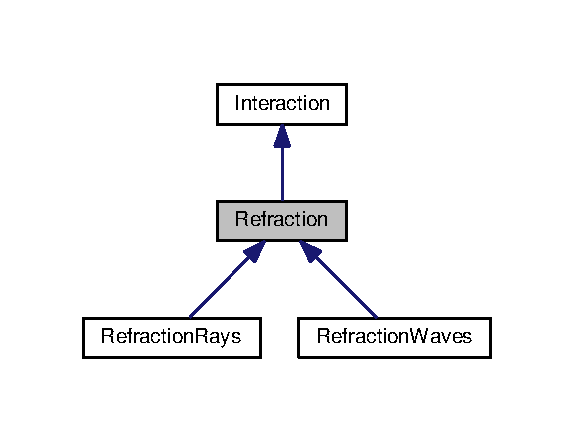
\includegraphics[width=276pt]{classRefraction__inherit__graph}
\end{center}
\end{figure}


Collaboration diagram for Refraction\+:\nopagebreak
\begin{figure}[H]
\begin{center}
\leavevmode
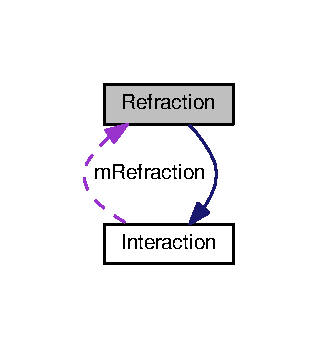
\includegraphics[width=152pt]{classRefraction__coll__graph}
\end{center}
\end{figure}
\subsection*{Public Member Functions}
\begin{DoxyCompactItemize}
\item 
virtual void {\bfseries perform} (\hyperlink{classLight}{Light} $\ast$l, \hyperlink{classElement}{Element} $\ast$const e)=0\hypertarget{classRefraction_aa32f9a0371dca4feb9984e999906c940}{}\label{classRefraction_aa32f9a0371dca4feb9984e999906c940}

\end{DoxyCompactItemize}
\subsection*{Additional Inherited Members}


\subsection{Detailed Description}
Most optical components are made out of Surfaces. 

The abstract base class \hyperlink{classRefraction}{Refraction} is the main class that is responsible for the special interaction refraction Beware\+: In general, this is done not at a surface but at an element

\begin{DoxyDate}{Date}
15.\+4.\+2017 
\end{DoxyDate}
\begin{DoxyAuthor}{Author}
Tobias Haist (\href{mailto:haist@ito.uni-stuttgart.de}{\tt haist@ito.\+uni-\/stuttgart.\+de}) 
\end{DoxyAuthor}


The documentation for this class was generated from the following files\+:\begin{DoxyCompactItemize}
\item 
\hyperlink{refraction_8h}{refraction.\+h}\item 
\hyperlink{refraction_8cc}{refraction.\+cc}\end{DoxyCompactItemize}

\hypertarget{classRefractionRays}{}\section{Refraction\+Rays Class Reference}
\label{classRefractionRays}\index{Refraction\+Rays@{Refraction\+Rays}}


Most optical components are made out of Surfaces.  




{\ttfamily \#include $<$refractionrays.\+h$>$}



Inheritance diagram for Refraction\+Rays\+:\nopagebreak
\begin{figure}[H]
\begin{center}
\leavevmode
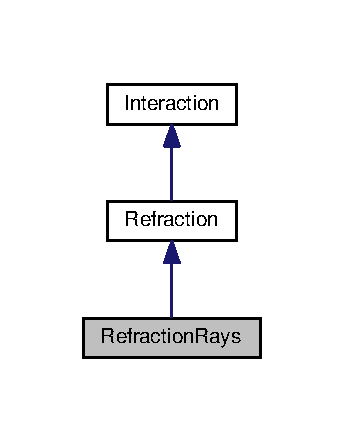
\includegraphics[width=165pt]{classRefractionRays__inherit__graph}
\end{center}
\end{figure}


Collaboration diagram for Refraction\+Rays\+:\nopagebreak
\begin{figure}[H]
\begin{center}
\leavevmode
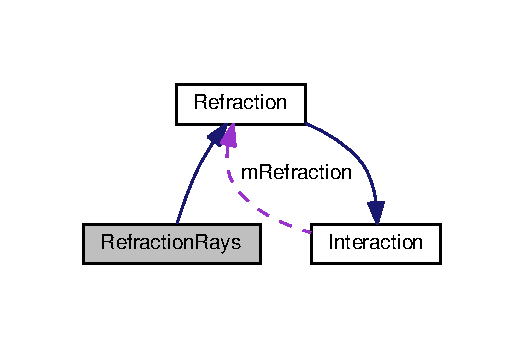
\includegraphics[width=252pt]{classRefractionRays__coll__graph}
\end{center}
\end{figure}
\subsection*{Public Member Functions}
\begin{DoxyCompactItemize}
\item 
virtual void \hyperlink{classRefractionRays_a275736609454ec99eb9557415ab4f8bd}{perform} (\hyperlink{classLight}{Light} $\ast$light, \hyperlink{classElement}{Element} $\ast$const element)
\begin{DoxyCompactList}\small\item\em perform refraction of rays through element \end{DoxyCompactList}\end{DoxyCompactItemize}
\subsection*{Additional Inherited Members}


\subsection{Detailed Description}
Most optical components are made out of Surfaces. 

The abstract base class \hyperlink{classRefraction}{Refraction} is the main class that is responsible for the special interaction refraction

\begin{DoxyDate}{Date}
15.\+4.\+2017 
\end{DoxyDate}
\begin{DoxyAuthor}{Author}
Tobias Haist (\href{mailto:haist@ito.uni-stuttgart.de}{\tt haist@ito.\+uni-\/stuttgart.\+de}) 
\end{DoxyAuthor}


\subsection{Member Function Documentation}
\index{Refraction\+Rays@{Refraction\+Rays}!perform@{perform}}
\index{perform@{perform}!Refraction\+Rays@{Refraction\+Rays}}
\subsubsection[{\texorpdfstring{perform(\+Light $\ast$light, Element $\ast$const element)}{perform(Light *light, Element *const element)}}]{\setlength{\rightskip}{0pt plus 5cm}void Refraction\+Rays\+::perform (
\begin{DoxyParamCaption}
\item[{{\bf Light} $\ast$}]{light, }
\item[{{\bf Element} $\ast$const}]{element}
\end{DoxyParamCaption}
)\hspace{0.3cm}{\ttfamily [virtual]}}\hypertarget{classRefractionRays_a275736609454ec99eb9557415ab4f8bd}{}\label{classRefractionRays_a275736609454ec99eb9557415ab4f8bd}


perform refraction of rays through element 


\begin{DoxyParams}{Parameters}
{\em light} & light to be traced through. Beware\+: S\+H\+O\+U\+LD BE Rays \\
\hline
{\em element} & the element we wish to trace through. \\
\hline
\end{DoxyParams}


Implements \hyperlink{classRefraction}{Refraction}.



The documentation for this class was generated from the following files\+:\begin{DoxyCompactItemize}
\item 
\hyperlink{refractionrays_8h}{refractionrays.\+h}\item 
\hyperlink{refractionrays_8cc}{refractionrays.\+cc}\end{DoxyCompactItemize}

\hypertarget{classRefractionWaves}{}\section{Refraction\+Waves Class Reference}
\label{classRefractionWaves}\index{Refraction\+Waves@{Refraction\+Waves}}


\hyperlink{classRefraction}{Refraction} of Waves.  




{\ttfamily \#include $<$refractionwaves.\+h$>$}



Inheritance diagram for Refraction\+Waves\+:\nopagebreak
\begin{figure}[H]
\begin{center}
\leavevmode
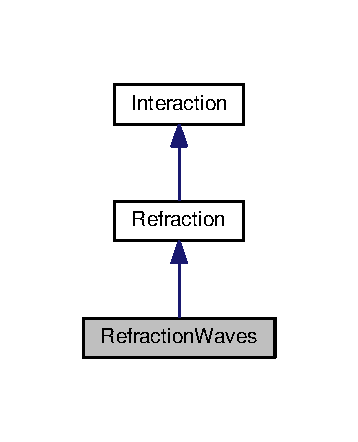
\includegraphics[width=172pt]{classRefractionWaves__inherit__graph}
\end{center}
\end{figure}


Collaboration diagram for Refraction\+Waves\+:\nopagebreak
\begin{figure}[H]
\begin{center}
\leavevmode
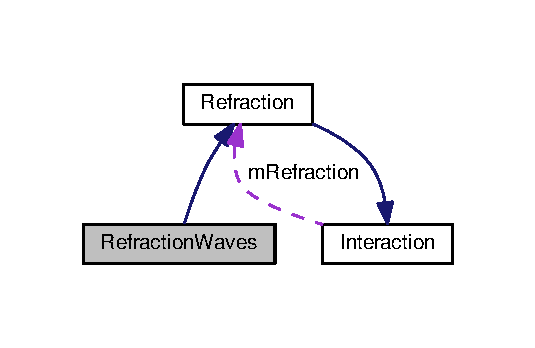
\includegraphics[width=257pt]{classRefractionWaves__coll__graph}
\end{center}
\end{figure}
\subsection*{Public Member Functions}
\begin{DoxyCompactItemize}
\item 
virtual void \hyperlink{classRefractionWaves_abff48838dcb27afdee215241a308f29f}{perform} (\hyperlink{classLight}{Light} $\ast$, \hyperlink{classElement}{Element} $\ast$const )
\begin{DoxyCompactList}\small\item\em trace a wave through element \end{DoxyCompactList}\end{DoxyCompactItemize}
\subsection*{Additional Inherited Members}


\subsection{Detailed Description}
\hyperlink{classRefraction}{Refraction} of Waves. 

The abstract base class \hyperlink{classRefraction}{Refraction} is the main class that is responsible for the special interaction refraction

\begin{DoxyDate}{Date}
15.\+4.\+2017 
\end{DoxyDate}
\begin{DoxyAuthor}{Author}
Tobias Haist (\href{mailto:haist@ito.uni-stuttgart.de}{\tt haist@ito.\+uni-\/stuttgart.\+de}) 
\end{DoxyAuthor}


\subsection{Member Function Documentation}
\index{Refraction\+Waves@{Refraction\+Waves}!perform@{perform}}
\index{perform@{perform}!Refraction\+Waves@{Refraction\+Waves}}
\subsubsection[{\texorpdfstring{perform(\+Light $\ast$, Element $\ast$const )}{perform(Light *, Element *const )}}]{\setlength{\rightskip}{0pt plus 5cm}void Refraction\+Waves\+::perform (
\begin{DoxyParamCaption}
\item[{{\bf Light} $\ast$}]{light, }
\item[{{\bf Element} $\ast$ const}]{element}
\end{DoxyParamCaption}
)\hspace{0.3cm}{\ttfamily [virtual]}}\hypertarget{classRefractionWaves_abff48838dcb27afdee215241a308f29f}{}\label{classRefractionWaves_abff48838dcb27afdee215241a308f29f}


trace a wave through element 


\begin{DoxyParams}{Parameters}
{\em light} & light to be traced through. Beware\+: S\+H\+O\+U\+LD BE waves \\
\hline
{\em element} & the element we wish to trace through. \\
\hline
\end{DoxyParams}


Implements \hyperlink{classRefraction}{Refraction}.



The documentation for this class was generated from the following files\+:\begin{DoxyCompactItemize}
\item 
\hyperlink{refractionwaves_8h}{refractionwaves.\+h}\item 
\hyperlink{refractionwaves_8cc}{refractionwaves.\+cc}\end{DoxyCompactItemize}

\hypertarget{classSurface}{}\section{Surface Class Reference}
\label{classSurface}\index{Surface@{Surface}}


Most optical components are made out of Surfaces.  




{\ttfamily \#include $<$surface.\+h$>$}



Inheritance diagram for Surface\+:\nopagebreak
\begin{figure}[H]
\begin{center}
\leavevmode
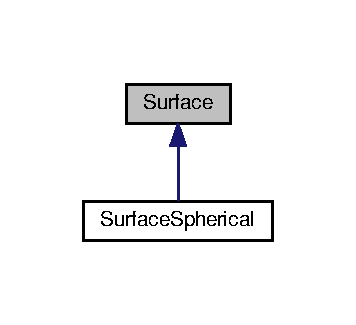
\includegraphics[width=171pt]{classSurface__inherit__graph}
\end{center}
\end{figure}


Collaboration diagram for Surface\+:
\nopagebreak
\begin{figure}[H]
\begin{center}
\leavevmode
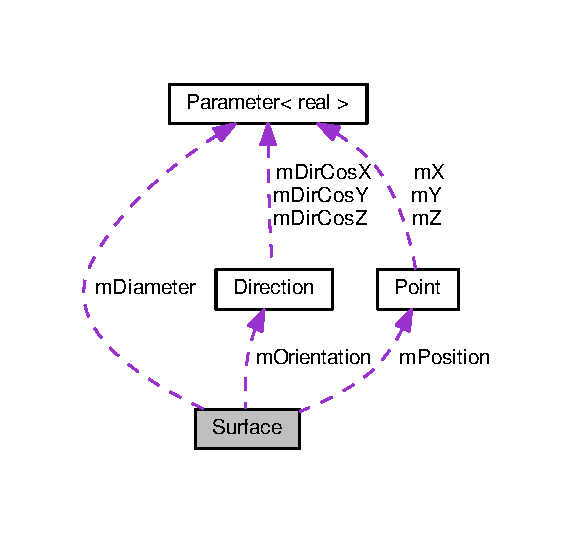
\includegraphics[width=276pt]{classSurface__coll__graph}
\end{center}
\end{figure}
\subsection*{Public Member Functions}
\begin{DoxyCompactItemize}
\item 
\hyperlink{classSurface_ac3d233e717ad7177f340765f07b4e7cb}{Surface} (\hyperlink{classPoint}{Point} pos, \hyperlink{classDirection}{Direction} dir, real diameter)
\begin{DoxyCompactList}\small\item\em ctor \end{DoxyCompactList}\item 
virtual \hyperlink{classSurface_a89de75c95cb550d432f3ea4ed1429db0}{$\sim$\+Surface} ()\hypertarget{classSurface_a89de75c95cb550d432f3ea4ed1429db0}{}\label{classSurface_a89de75c95cb550d432f3ea4ed1429db0}

\begin{DoxyCompactList}\small\item\em dtor \end{DoxyCompactList}\end{DoxyCompactItemize}
\subsection*{Protected Attributes}
\begin{DoxyCompactItemize}
\item 
\hyperlink{classPoint}{Point} \hyperlink{classSurface_aedc39cb43d82a98b61eb45844de57658}{m\+Position}\hypertarget{classSurface_aedc39cb43d82a98b61eb45844de57658}{}\label{classSurface_aedc39cb43d82a98b61eb45844de57658}

\begin{DoxyCompactList}\small\item\em Position in Space (global coordinates) \end{DoxyCompactList}\item 
\hyperlink{classDirection}{Direction} \hyperlink{classSurface_a11e958be47f8f0aec30dac7526311507}{m\+Orientation}\hypertarget{classSurface_a11e958be47f8f0aec30dac7526311507}{}\label{classSurface_a11e958be47f8f0aec30dac7526311507}

\begin{DoxyCompactList}\small\item\em orientation in Space (global coordinates) \end{DoxyCompactList}\item 
\hyperlink{classParameter}{Parameter}$<$ real $>$ \hyperlink{classSurface_ae00d3ff70c7fd76b99c405f5c0196ebf}{m\+Diameter}\hypertarget{classSurface_ae00d3ff70c7fd76b99c405f5c0196ebf}{}\label{classSurface_ae00d3ff70c7fd76b99c405f5c0196ebf}

\begin{DoxyCompactList}\small\item\em Diameter of usable surface (inner circle) \end{DoxyCompactList}\end{DoxyCompactItemize}


\subsection{Detailed Description}
Most optical components are made out of Surfaces. 

Most often, elements are lenses or mirrors. These elements are \char`\"{}elements with (or consisting of) surfaces\char`\"{}.

The abstract base class \hyperlink{classSurface}{Surface} is the core for the implementation of all kinds of surfaces.

\begin{DoxyDate}{Date}
07.\+4.\+2017 
\end{DoxyDate}
\begin{DoxyAuthor}{Author}
Tobias Haist (\href{mailto:haist@ito.uni-stuttgart.de}{\tt haist@ito.\+uni-\/stuttgart.\+de}) 
\end{DoxyAuthor}


\subsection{Constructor \& Destructor Documentation}
\index{Surface@{Surface}!Surface@{Surface}}
\index{Surface@{Surface}!Surface@{Surface}}
\subsubsection[{\texorpdfstring{Surface(\+Point pos, Direction dir, real diameter)}{Surface(Point pos, Direction dir, real diameter)}}]{\setlength{\rightskip}{0pt plus 5cm}Surface\+::\+Surface (
\begin{DoxyParamCaption}
\item[{{\bf Point}}]{pos, }
\item[{{\bf Direction}}]{dir, }
\item[{real}]{diameter}
\end{DoxyParamCaption}
)}\hypertarget{classSurface_ac3d233e717ad7177f340765f07b4e7cb}{}\label{classSurface_ac3d233e717ad7177f340765f07b4e7cb}


ctor 


\begin{DoxyParams}{Parameters}
{\em pos} & Position of \hyperlink{classSurface}{Surface} in global coordinates \\
\hline
{\em dir} & orientation of \hyperlink{classSurface}{Surface} with respect to global coordinate system \\
\hline
{\em diameter} & diameter of surface \\
\hline
\end{DoxyParams}


The documentation for this class was generated from the following files\+:\begin{DoxyCompactItemize}
\item 
\hyperlink{surface_8h}{surface.\+h}\item 
\hyperlink{surface_8cc}{surface.\+cc}\end{DoxyCompactItemize}

\hypertarget{classSurfaceSpherical}{}\section{Surface\+Spherical Class Reference}
\label{classSurfaceSpherical}\index{Surface\+Spherical@{Surface\+Spherical}}


Most optical components are made out of Surfaces.  




{\ttfamily \#include $<$surfacespherical.\+h$>$}



Inheritance diagram for Surface\+Spherical\+:\nopagebreak
\begin{figure}[H]
\begin{center}
\leavevmode
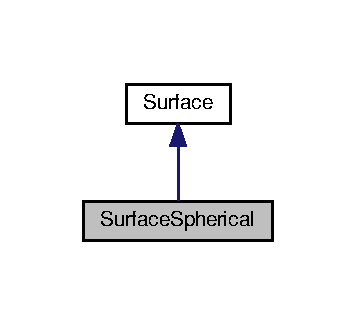
\includegraphics[width=171pt]{classSurfaceSpherical__inherit__graph}
\end{center}
\end{figure}


Collaboration diagram for Surface\+Spherical\+:
\nopagebreak
\begin{figure}[H]
\begin{center}
\leavevmode
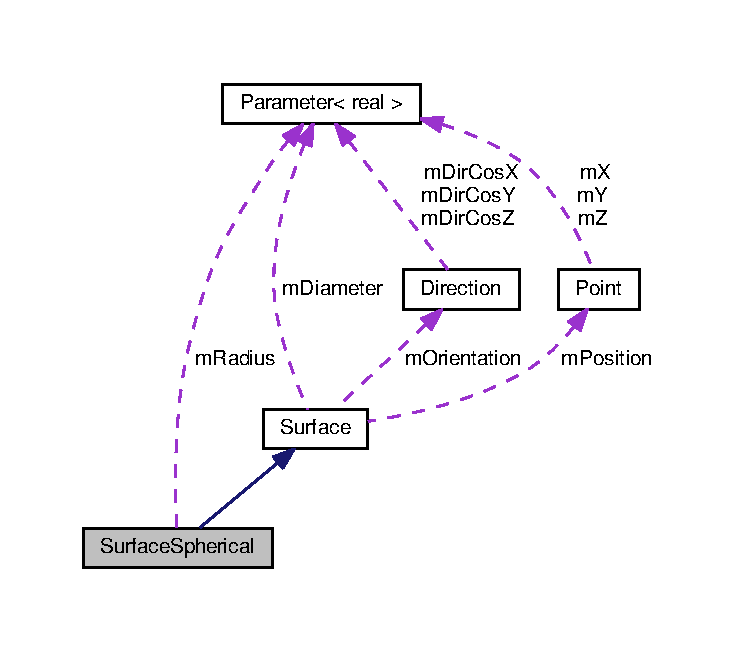
\includegraphics[width=350pt]{classSurfaceSpherical__coll__graph}
\end{center}
\end{figure}
\subsection*{Public Member Functions}
\begin{DoxyCompactItemize}
\item 
\hyperlink{classSurfaceSpherical_ab316d1d811ac3ef1032dcf6da0fe0763}{Surface\+Spherical} (real \hyperlink{classSurfaceSpherical_a056c0dba260183f9a2bc555e94310166}{m\+Radius}, real diameter, \hyperlink{classPoint}{Point} p)
\begin{DoxyCompactList}\small\item\em ctor \end{DoxyCompactList}\end{DoxyCompactItemize}
\subsection*{Protected Attributes}
\begin{DoxyCompactItemize}
\item 
\hyperlink{classParameter}{Parameter}$<$ real $>$ \hyperlink{classSurfaceSpherical_a056c0dba260183f9a2bc555e94310166}{m\+Radius}\hypertarget{classSurfaceSpherical_a056c0dba260183f9a2bc555e94310166}{}\label{classSurfaceSpherical_a056c0dba260183f9a2bc555e94310166}

\begin{DoxyCompactList}\small\item\em Radius of curvature. \end{DoxyCompactList}\end{DoxyCompactItemize}


\subsection{Detailed Description}
Most optical components are made out of Surfaces. 

Most often, elements are lenses or mirrors. These elements are \char`\"{}elements with (or consisting of) surfaces\char`\"{}.

The abstract base class \hyperlink{classSurface}{Surface} is the core for the implementation of all kinds of surfaces.

\begin{DoxyDate}{Date}
15.\+4.\+2017 
\end{DoxyDate}
\begin{DoxyAuthor}{Author}
Tobias Haist (\href{mailto:haist@ito.uni-stuttgart.de}{\tt haist@ito.\+uni-\/stuttgart.\+de}) 
\end{DoxyAuthor}


\subsection{Constructor \& Destructor Documentation}
\index{Surface\+Spherical@{Surface\+Spherical}!Surface\+Spherical@{Surface\+Spherical}}
\index{Surface\+Spherical@{Surface\+Spherical}!Surface\+Spherical@{Surface\+Spherical}}
\subsubsection[{\texorpdfstring{Surface\+Spherical(real m\+Radius, real diameter, Point p)}{SurfaceSpherical(real mRadius, real diameter, Point p)}}]{\setlength{\rightskip}{0pt plus 5cm}Surface\+Spherical\+::\+Surface\+Spherical (
\begin{DoxyParamCaption}
\item[{real}]{m\+Radius, }
\item[{real}]{diameter, }
\item[{{\bf Point}}]{p}
\end{DoxyParamCaption}
)}\hypertarget{classSurfaceSpherical_ab316d1d811ac3ef1032dcf6da0fe0763}{}\label{classSurfaceSpherical_ab316d1d811ac3ef1032dcf6da0fe0763}


ctor 


\begin{DoxyParams}{Parameters}
{\em radius} & radius of curvature \\
\hline
{\em diameter} & diameter of surface \\
\hline
{\em p} & Position of Scheitel in Space \\
\hline
\end{DoxyParams}


The documentation for this class was generated from the following files\+:\begin{DoxyCompactItemize}
\item 
\hyperlink{surfacespherical_8h}{surfacespherical.\+h}\item 
\hyperlink{surfacespherical_8cc}{surfacespherical.\+cc}\end{DoxyCompactItemize}

\hypertarget{classTraceOpenError}{}\section{Trace\+Open\+Error Class Reference}
\label{classTraceOpenError}\index{Trace\+Open\+Error@{Trace\+Open\+Error}}


Inheritance diagram for Trace\+Open\+Error\+:
\nopagebreak
\begin{figure}[H]
\begin{center}
\leavevmode
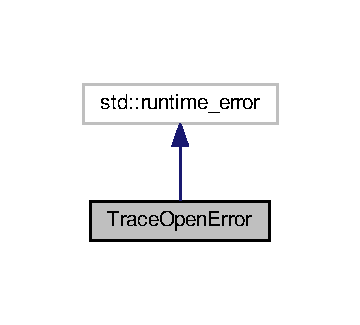
\includegraphics[width=173pt]{classTraceOpenError__inherit__graph}
\end{center}
\end{figure}


Collaboration diagram for Trace\+Open\+Error\+:
\nopagebreak
\begin{figure}[H]
\begin{center}
\leavevmode
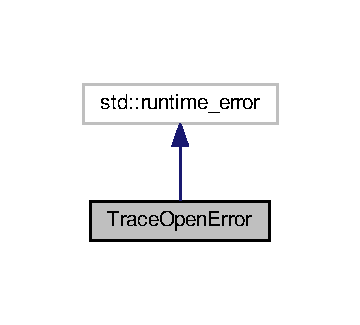
\includegraphics[width=173pt]{classTraceOpenError__coll__graph}
\end{center}
\end{figure}
\subsection*{Public Member Functions}
\begin{DoxyCompactItemize}
\item 
{\bfseries Trace\+Open\+Error} (std\+::string const \&s, int nr=0)\hypertarget{classTraceOpenError_a22262d6be0a9400616618e893dff276e}{}\label{classTraceOpenError_a22262d6be0a9400616618e893dff276e}

\end{DoxyCompactItemize}
\subsection*{Public Attributes}
\begin{DoxyCompactItemize}
\item 
int {\bfseries errno}\hypertarget{classTraceOpenError_a9e8f0f4ff3cb084f978e9466dcb9bf92}{}\label{classTraceOpenError_a9e8f0f4ff3cb084f978e9466dcb9bf92}

\end{DoxyCompactItemize}


The documentation for this class was generated from the following file\+:\begin{DoxyCompactItemize}
\item 
\hyperlink{traceopenerror_8h}{traceopenerror.\+h}\end{DoxyCompactItemize}

\hypertarget{classTracing}{}\section{Tracing Class Reference}
\label{classTracing}\index{Tracing@{Tracing}}


Most optical components are made out of Surfaces.  




{\ttfamily \#include $<$tracing.\+h$>$}



Collaboration diagram for Tracing\+:\nopagebreak
\begin{figure}[H]
\begin{center}
\leavevmode
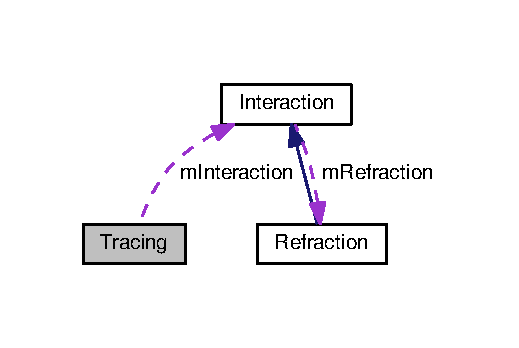
\includegraphics[width=249pt]{classTracing__coll__graph}
\end{center}
\end{figure}
\subsection*{Public Member Functions}
\begin{DoxyCompactItemize}
\item 
\hyperlink{classTracing_aa1207cbaf59ba3f2c200a80cd137b216}{Tracing} ()\hypertarget{classTracing_aa1207cbaf59ba3f2c200a80cd137b216}{}\label{classTracing_aa1207cbaf59ba3f2c200a80cd137b216}

\begin{DoxyCompactList}\small\item\em ctor \end{DoxyCompactList}\item 
\hyperlink{classTracing_a699e507b9d71ca86ff4759798f67a58b}{$\sim$\+Tracing} ()\hypertarget{classTracing_a699e507b9d71ca86ff4759798f67a58b}{}\label{classTracing_a699e507b9d71ca86ff4759798f67a58b}

\begin{DoxyCompactList}\small\item\em dtor \end{DoxyCompactList}\item 
void \hyperlink{classTracing_a0d1449364b93a2fab5d9a8f4a10f5a3a}{set\+Interaction} (\hyperlink{classInteraction}{Interaction} $\ast$const i)
\begin{DoxyCompactList}\small\item\em set the interation to i \end{DoxyCompactList}\item 
void \hyperlink{classTracing_aa347dfabff1a62e587004b671e570844}{trace} (\hyperlink{classLight}{Light} $\ast$l, \hyperlink{classOpticalSystem}{Optical\+System} $\ast$const s) const 
\begin{DoxyCompactList}\small\item\em trace light through a complete system \end{DoxyCompactList}\item 
void \hyperlink{classTracing_af01d7dd435e2ce61fdd0b3c56da8b001}{init} (\hyperlink{classLight}{Light} $\ast$const l)
\begin{DoxyCompactList}\small\item\em init the interactions based on light model \end{DoxyCompactList}\end{DoxyCompactItemize}
\subsection*{Protected Attributes}
\begin{DoxyCompactItemize}
\item 
\hyperlink{classInteraction}{Interaction} $\ast$ \hyperlink{classTracing_a5f7a022b92a31067dd44c908196bbc16}{m\+Interaction}\hypertarget{classTracing_a5f7a022b92a31067dd44c908196bbc16}{}\label{classTracing_a5f7a022b92a31067dd44c908196bbc16}

\begin{DoxyCompactList}\small\item\em This is used for handling interactions. \end{DoxyCompactList}\end{DoxyCompactItemize}


\subsection{Detailed Description}
Most optical components are made out of Surfaces. 

/// The abstract base class \hyperlink{classTracing}{Tracing} is the main container for propagation and interaction.

\begin{DoxyDate}{Date}
15.\+4.\+2017 
\end{DoxyDate}
\begin{DoxyAuthor}{Author}
Tobias Haist (\href{mailto:haist@ito.uni-stuttgart.de}{\tt haist@ito.\+uni-\/stuttgart.\+de}) 
\end{DoxyAuthor}


\subsection{Member Function Documentation}
\index{Tracing@{Tracing}!init@{init}}
\index{init@{init}!Tracing@{Tracing}}
\subsubsection[{\texorpdfstring{init(\+Light $\ast$const l)}{init(Light *const l)}}]{\setlength{\rightskip}{0pt plus 5cm}void Tracing\+::init (
\begin{DoxyParamCaption}
\item[{{\bf Light} $\ast$const}]{l}
\end{DoxyParamCaption}
)}\hypertarget{classTracing_af01d7dd435e2ce61fdd0b3c56da8b001}{}\label{classTracing_af01d7dd435e2ce61fdd0b3c56da8b001}


init the interactions based on light model 


\begin{DoxyParams}{Parameters}
{\em l} & light based on which all interactions are to be set \\
\hline
\end{DoxyParams}
\index{Tracing@{Tracing}!set\+Interaction@{set\+Interaction}}
\index{set\+Interaction@{set\+Interaction}!Tracing@{Tracing}}
\subsubsection[{\texorpdfstring{set\+Interaction(\+Interaction $\ast$const i)}{setInteraction(Interaction *const i)}}]{\setlength{\rightskip}{0pt plus 5cm}void Tracing\+::set\+Interaction (
\begin{DoxyParamCaption}
\item[{{\bf Interaction} $\ast$const}]{i}
\end{DoxyParamCaption}
)}\hypertarget{classTracing_a0d1449364b93a2fab5d9a8f4a10f5a3a}{}\label{classTracing_a0d1449364b93a2fab5d9a8f4a10f5a3a}


set the interation to i 


\begin{DoxyParams}{Parameters}
{\em i} & interaction that will be used for tracing through \\
\hline
\end{DoxyParams}
\index{Tracing@{Tracing}!trace@{trace}}
\index{trace@{trace}!Tracing@{Tracing}}
\subsubsection[{\texorpdfstring{trace(\+Light $\ast$l, Optical\+System $\ast$const s) const }{trace(Light *l, OpticalSystem *const s) const }}]{\setlength{\rightskip}{0pt plus 5cm}void Tracing\+::trace (
\begin{DoxyParamCaption}
\item[{{\bf Light} $\ast$}]{l, }
\item[{{\bf Optical\+System} $\ast$const}]{s}
\end{DoxyParamCaption}
) const}\hypertarget{classTracing_aa347dfabff1a62e587004b671e570844}{}\label{classTracing_aa347dfabff1a62e587004b671e570844}


trace light through a complete system 


\begin{DoxyParams}{Parameters}
{\em l} & light to be traced \\
\hline
{\em s} & optical system through which we want to trace \\
\hline
\end{DoxyParams}


The documentation for this class was generated from the following files\+:\begin{DoxyCompactItemize}
\item 
\hyperlink{tracing_8h}{tracing.\+h}\item 
\hyperlink{tracing_8cc}{tracing.\+cc}\end{DoxyCompactItemize}

\hypertarget{classWave}{}\section{Wave Class Reference}
\label{classWave}\index{Wave@{Wave}}


\hyperlink{classRay}{Ray} manages optical (polarized or unpolarized) Rays.  




{\ttfamily \#include $<$wave.\+h$>$}



Inheritance diagram for Wave\+:\nopagebreak
\begin{figure}[H]
\begin{center}
\leavevmode
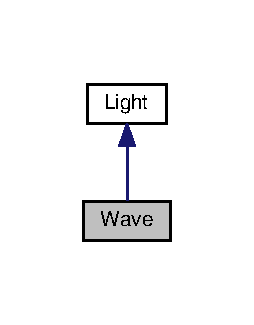
\includegraphics[width=122pt]{classWave__inherit__graph}
\end{center}
\end{figure}


Collaboration diagram for Wave\+:\nopagebreak
\begin{figure}[H]
\begin{center}
\leavevmode
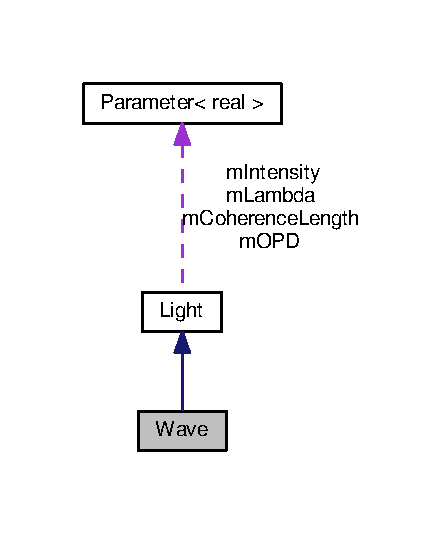
\includegraphics[width=213pt]{classWave__coll__graph}
\end{center}
\end{figure}
\subsection*{Public Member Functions}
\begin{DoxyCompactItemize}
\item 
\hyperlink{classWave_a3d8144ec0d6c0b0ede77ff59f54471aa}{Wave} ()\hypertarget{classWave_a3d8144ec0d6c0b0ede77ff59f54471aa}{}\label{classWave_a3d8144ec0d6c0b0ede77ff59f54471aa}

\begin{DoxyCompactList}\small\item\em std ctor \end{DoxyCompactList}\end{DoxyCompactItemize}
\subsection*{Additional Inherited Members}


\subsection{Detailed Description}
\hyperlink{classRay}{Ray} manages optical (polarized or unpolarized) Rays. 

This is the basic class for representing light in a simple scalar waevoptical model. The wave will be implemented with conventional Arrays and equidistant points Other waveoptical methods should be derived from this class

\begin{DoxyDate}{Date}
07.\+4.\+2017 
\end{DoxyDate}
\begin{DoxyAuthor}{Author}
Tobias Haist (\href{mailto:haist@ito.uni-stuttgart.de}{\tt haist@ito.\+uni-\/stuttgart.\+de}) 
\end{DoxyAuthor}


The documentation for this class was generated from the following files\+:\begin{DoxyCompactItemize}
\item 
\hyperlink{wave_8h}{wave.\+h}\item 
\hyperlink{wave_8cc}{wave.\+cc}\end{DoxyCompactItemize}

\chapter{File Documentation}
\hypertarget{array_8cc}{}\section{array.\+cc File Reference}
\label{array_8cc}\index{array.\+cc@{array.\+cc}}
{\ttfamily \#include $<$fstream$>$}\\*
{\ttfamily \#include $<$stdio.\+h$>$}\\*
{\ttfamily \#include $<$stdlib.\+h$>$}\\*
{\ttfamily \#include \char`\"{}array.\+h\char`\"{}}\\*
{\ttfamily \#include \char`\"{}error.\+h\char`\"{}}\\*
Include dependency graph for array.\+cc\+:\nopagebreak
\begin{figure}[H]
\begin{center}
\leavevmode
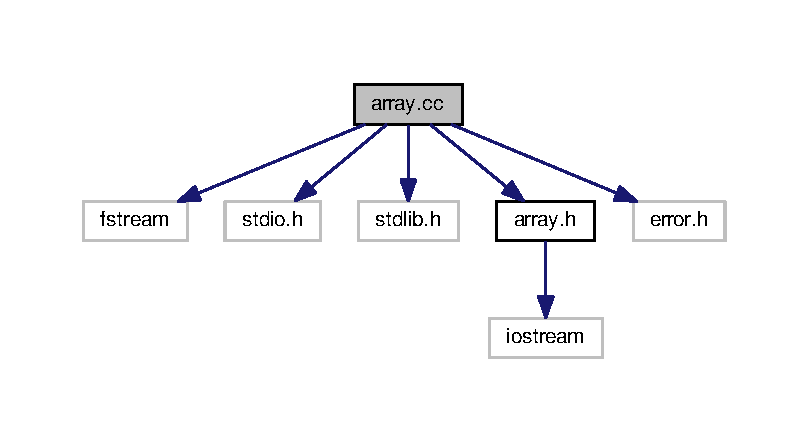
\includegraphics[width=350pt]{array_8cc__incl}
\end{center}
\end{figure}
\subsection*{Macros}
\begin{DoxyCompactItemize}
\item 
\#define {\bfseries I\+T\+O\+A\+R\+R\+A\+Y\+D\+E\+B\+UG}~0\hypertarget{array_8cc_a1d894c7bb1109037cb9935f5ff8220b0}{}\label{array_8cc_a1d894c7bb1109037cb9935f5ff8220b0}

\end{DoxyCompactItemize}

\hypertarget{array_8h}{}\section{array.\+h File Reference}
\label{array_8h}\index{array.\+h@{array.\+h}}


include file for template Class \hyperlink{classArray}{Array}  


{\ttfamily \#include $<$iostream$>$}\\*
Include dependency graph for array.\+h\+:\nopagebreak
\begin{figure}[H]
\begin{center}
\leavevmode
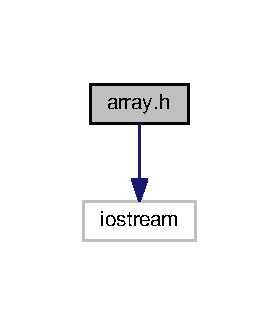
\includegraphics[width=134pt]{array_8h__incl}
\end{center}
\end{figure}
This graph shows which files directly or indirectly include this file\+:\nopagebreak
\begin{figure}[H]
\begin{center}
\leavevmode
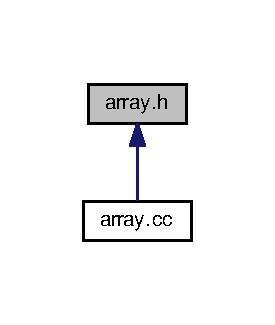
\includegraphics[width=132pt]{array_8h__dep__incl}
\end{center}
\end{figure}
\subsection*{Classes}
\begin{DoxyCompactItemize}
\item 
class \hyperlink{classArray}{Array$<$ Type $>$}
\begin{DoxyCompactList}\small\item\em Management of a 2D (and 1D) Arrays of different Type. \end{DoxyCompactList}\end{DoxyCompactItemize}
\subsection*{Macros}
\begin{DoxyCompactItemize}
\item 
\#define \hyperlink{array_8h_a5995122d2b869296f4cc48be46dbe1d6}{A\+R\+R\+A\+Y\+D\+E\+B\+UG}~0
\end{DoxyCompactItemize}


\subsection{Detailed Description}
include file for template Class \hyperlink{classArray}{Array} 

\begin{DoxyDate}{Date}
27.\+5.\+2007 
\end{DoxyDate}
\begin{DoxyAuthor}{Author}
Tobias Haist (\href{mailto:haist@ito.uni-stuttgart.de}{\tt haist@ito.\+uni-\/stuttgart.\+de}) Copyright Institute of Applied Optics, University of Stuttgart I\+TO 1999 Paffenwaldring 9 70569 Stuttgart Germany
\end{DoxyAuthor}
This is a rewrite of a very old class (programmed in 1999) by me. 

\subsection{Macro Definition Documentation}
\index{array.\+h@{array.\+h}!A\+R\+R\+A\+Y\+D\+E\+B\+UG@{A\+R\+R\+A\+Y\+D\+E\+B\+UG}}
\index{A\+R\+R\+A\+Y\+D\+E\+B\+UG@{A\+R\+R\+A\+Y\+D\+E\+B\+UG}!array.\+h@{array.\+h}}
\subsubsection[{\texorpdfstring{A\+R\+R\+A\+Y\+D\+E\+B\+UG}{ARRAYDEBUG}}]{\setlength{\rightskip}{0pt plus 5cm}\#define A\+R\+R\+A\+Y\+D\+E\+B\+UG~0}\hypertarget{array_8h_a5995122d2b869296f4cc48be46dbe1d6}{}\label{array_8h_a5995122d2b869296f4cc48be46dbe1d6}
To be implemented
\begin{DoxyItemize}
\item wrap 2pi
\item T\+I\+FF Funktion if defined L\+I\+B\+T\+I\+FF
\item Bildverarbeitung\+:
\begin{DoxyItemize}
\item Gaussfilter
\item Mittelwertfilter
\item Median
\item Threshold globale
\item Threshold local
\item Threshold bernsen
\item Gamma
\item Schwerpunkt
\item N\+GC
\item S\+AE
\item Aufl�sung Reduzieren um Faktor 2
\item evtl. die ganzen Funktionen, die netpbm bietet (nur wenn auch Windwos)
\item evtl. die ganzen Funktionen von imagick (nur wenn auch Windows)
\item search one peak
\item locate one peak
\item pce
\item draw circle
\item draw rectangle
\end{DoxyItemize}
\item Nullstellensuche
\item Ableitung
\item Matrix $\ast$ vektor
\item Matrix $\ast$ Matrix
\item SV Zerlegung L\+GS
\item Hanning Window
\item Bartlett Window
\item Zeropadding
\item shift
\item Rekonstruktion\+Phasenholo
\item Rekonstruktion\+Amplitudenholo
\item Propagation ebene Wellen
\item sinc
\item rect
\item L\+CD
\item Airy
\item PV Fehler
\item R\+MS Fehler
\item Marcheval usw.
\item Zernike Fit
\item gnuplot
\item Polynomfit
\item Curve\+Fit
\item y oder y akkumulieren
\item Korrelation
\item S\+AE 
\end{DoxyItemize}
\hypertarget{direction_8h}{}\section{direction.\+h File Reference}
\label{direction_8h}\index{direction.\+h@{direction.\+h}}


include file for class \hyperlink{classDirection}{Direction}  


{\ttfamily \#include \char`\"{}basicdefinitions.\+h\char`\"{}}\\*
{\ttfamily \#include \char`\"{}parameter.\+h\char`\"{}}\\*
{\ttfamily \#include $<$iostream$>$}\\*
Include dependency graph for direction.\+h\+:
\nopagebreak
\begin{figure}[H]
\begin{center}
\leavevmode
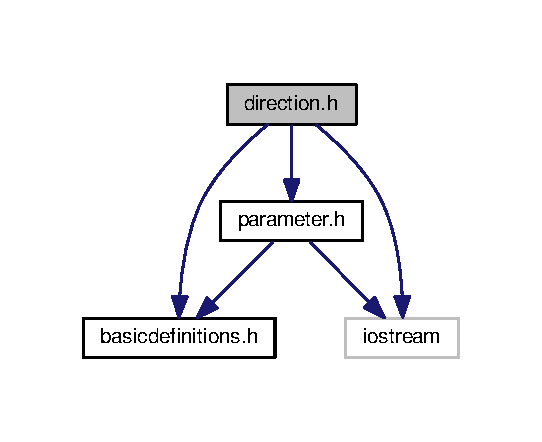
\includegraphics[width=260pt]{direction_8h__incl}
\end{center}
\end{figure}
This graph shows which files directly or indirectly include this file\+:\nopagebreak
\begin{figure}[H]
\begin{center}
\leavevmode
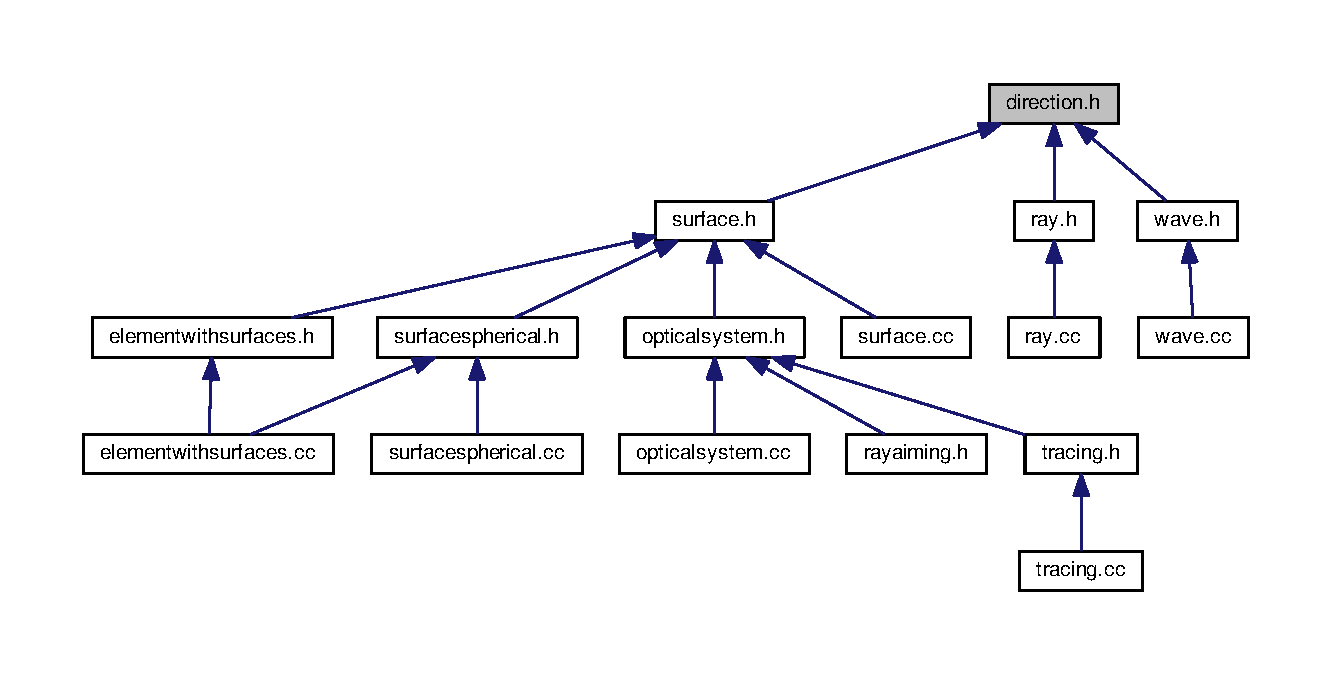
\includegraphics[width=350pt]{direction_8h__dep__incl}
\end{center}
\end{figure}
\subsection*{Classes}
\begin{DoxyCompactItemize}
\item 
class \hyperlink{classDirection}{Direction}
\begin{DoxyCompactList}\small\item\em \hyperlink{classDirection}{Direction} manages Directions/\+Orientations in Space. \end{DoxyCompactList}\end{DoxyCompactItemize}


\subsection{Detailed Description}
include file for class \hyperlink{classDirection}{Direction} 

\begin{DoxyDate}{Date}
07.\+04.\+2017 
\end{DoxyDate}
\begin{DoxyAuthor}{Author}
Tobias Haist (\href{mailto:haist@ito.uni-stuttgart.de}{\tt haist@ito.\+uni-\/stuttgart.\+de}) Institute of Applied Optics, University of Stuttgart I\+TO Paffenwaldring 9 70569 Stuttgart Germany 
\end{DoxyAuthor}

\hypertarget{element_8cc}{}\section{element.\+cc File Reference}
\label{element_8cc}\index{element.\+cc@{element.\+cc}}


class \hyperlink{classElement}{Element}  


{\ttfamily \#include \char`\"{}element.\+h\char`\"{}}\\*
Include dependency graph for element.\+cc\+:
\nopagebreak
\begin{figure}[H]
\begin{center}
\leavevmode
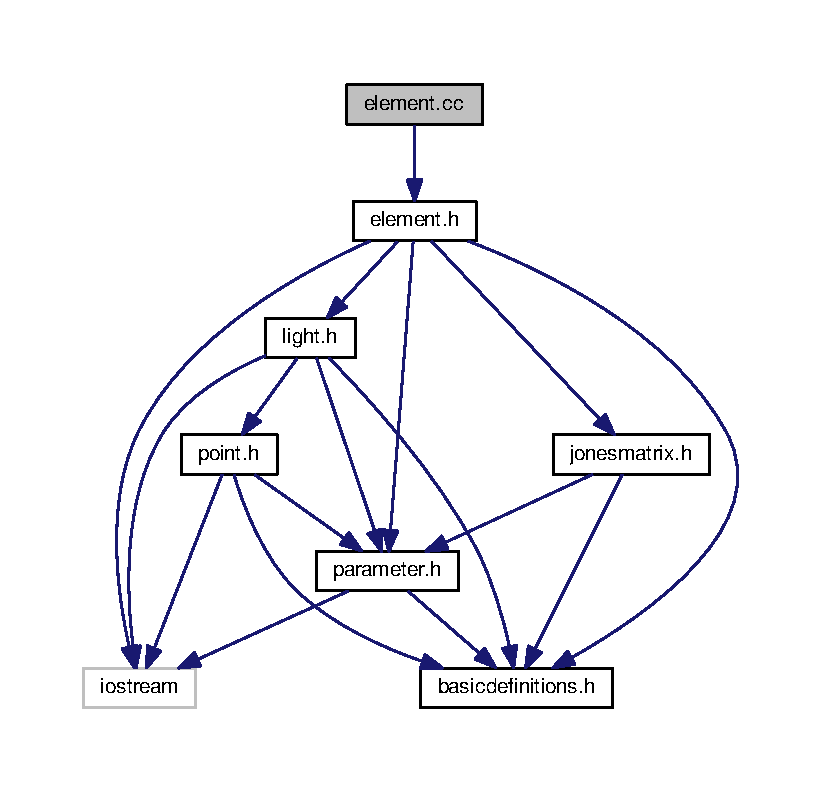
\includegraphics[width=350pt]{element_8cc__incl}
\end{center}
\end{figure}


\subsection{Detailed Description}
class \hyperlink{classElement}{Element} 

\begin{DoxyDate}{Date}
07.\+04.\+2017 
\end{DoxyDate}
\begin{DoxyAuthor}{Author}
Tobias Haist (\href{mailto:haist@ito.uni-stuttgart.de}{\tt haist@ito.\+uni-\/stuttgart.\+de}) Institute of Applied Optics, University of Stuttgart I\+TO Paffenwaldring 9 70569 Stuttgart Germany 
\end{DoxyAuthor}

\hypertarget{element_8h}{}\section{element.\+h File Reference}
\label{element_8h}\index{element.\+h@{element.\+h}}


include file for class \hyperlink{classElement}{Element}  


{\ttfamily \#include \char`\"{}basicdefinitions.\+h\char`\"{}}\\*
{\ttfamily \#include \char`\"{}light.\+h\char`\"{}}\\*
{\ttfamily \#include \char`\"{}parameter.\+h\char`\"{}}\\*
{\ttfamily \#include \char`\"{}jonesmatrix.\+h\char`\"{}}\\*
{\ttfamily \#include $<$iostream$>$}\\*
Include dependency graph for element.\+h\+:
\nopagebreak
\begin{figure}[H]
\begin{center}
\leavevmode
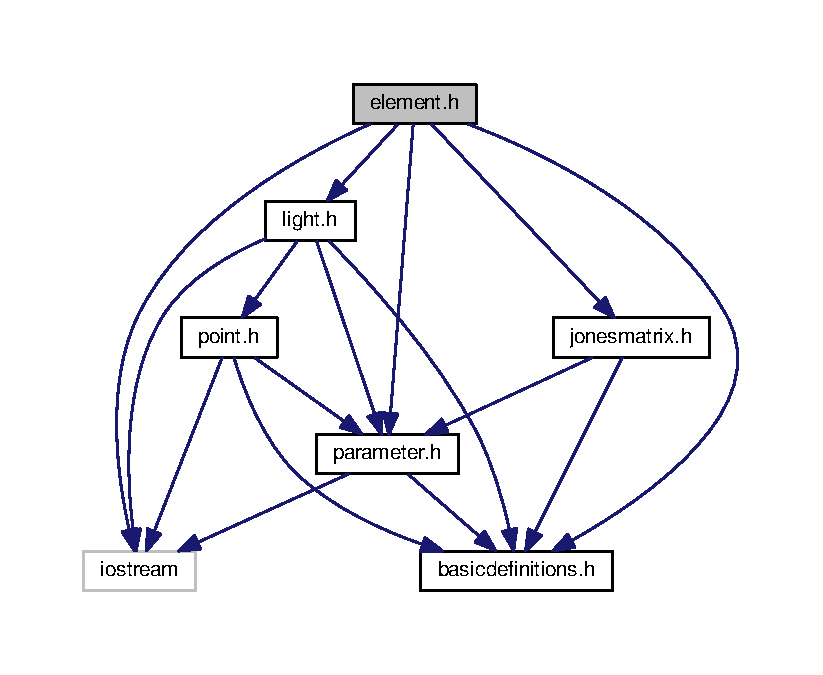
\includegraphics[width=350pt]{element_8h__incl}
\end{center}
\end{figure}
This graph shows which files directly or indirectly include this file\+:\nopagebreak
\begin{figure}[H]
\begin{center}
\leavevmode
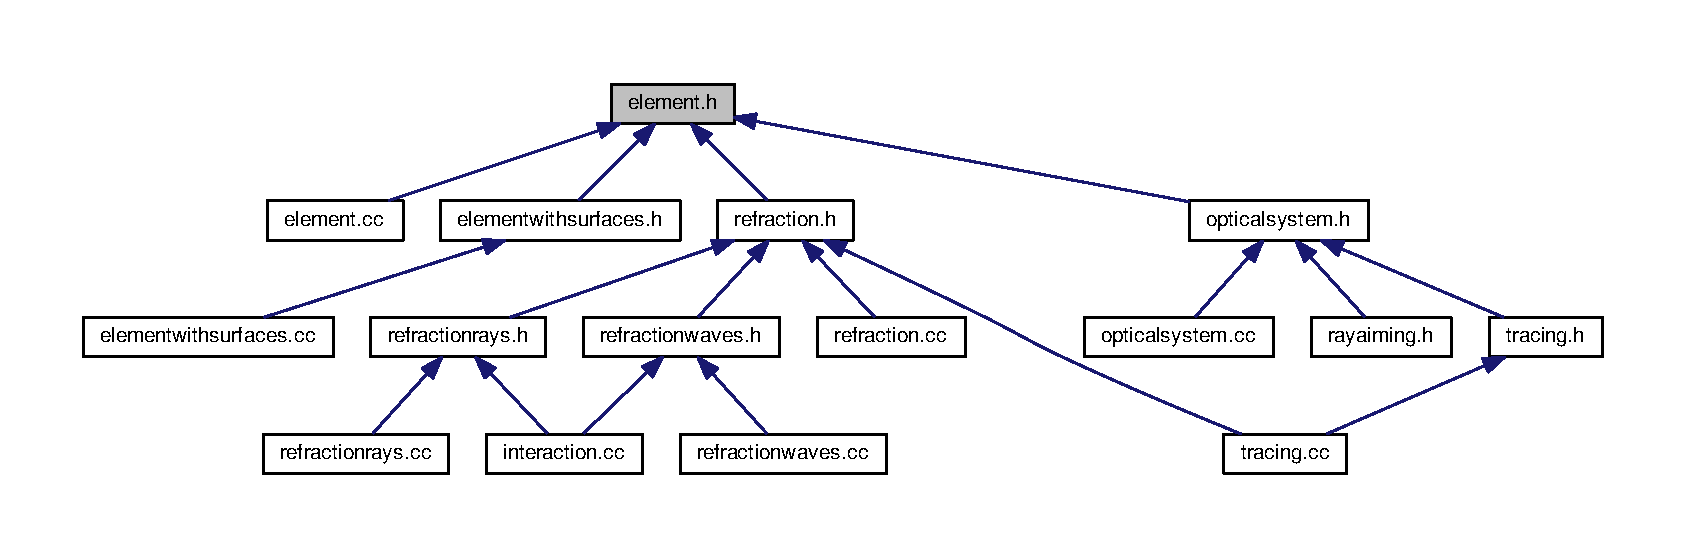
\includegraphics[width=350pt]{element_8h__dep__incl}
\end{center}
\end{figure}
\subsection*{Classes}
\begin{DoxyCompactItemize}
\item 
class \hyperlink{classElement}{Element}
\begin{DoxyCompactList}\small\item\em \hyperlink{classElement}{Element} represents an element/component of an optical system. \end{DoxyCompactList}\end{DoxyCompactItemize}


\subsection{Detailed Description}
include file for class \hyperlink{classElement}{Element} 

\begin{DoxyDate}{Date}
07.\+04.\+2017 
\end{DoxyDate}
\begin{DoxyAuthor}{Author}
Tobias Haist (\href{mailto:haist@ito.uni-stuttgart.de}{\tt haist@ito.\+uni-\/stuttgart.\+de}) Institute of Applied Optics, University of Stuttgart I\+TO Paffenwaldring 9 70569 Stuttgart Germany 
\end{DoxyAuthor}

\hypertarget{elementwithsurfaces_8cc}{}\section{elementwithsurfaces.\+cc File Reference}
\label{elementwithsurfaces_8cc}\index{elementwithsurfaces.\+cc@{elementwithsurfaces.\+cc}}


class \hyperlink{classElementWithSurfaces}{Element\+With\+Surfaces}  


{\ttfamily \#include \char`\"{}elementwithsurfaces.\+h\char`\"{}}\\*
{\ttfamily \#include \char`\"{}surfacespherical.\+h\char`\"{}}\\*
Include dependency graph for elementwithsurfaces.\+cc\+:
\nopagebreak
\begin{figure}[H]
\begin{center}
\leavevmode
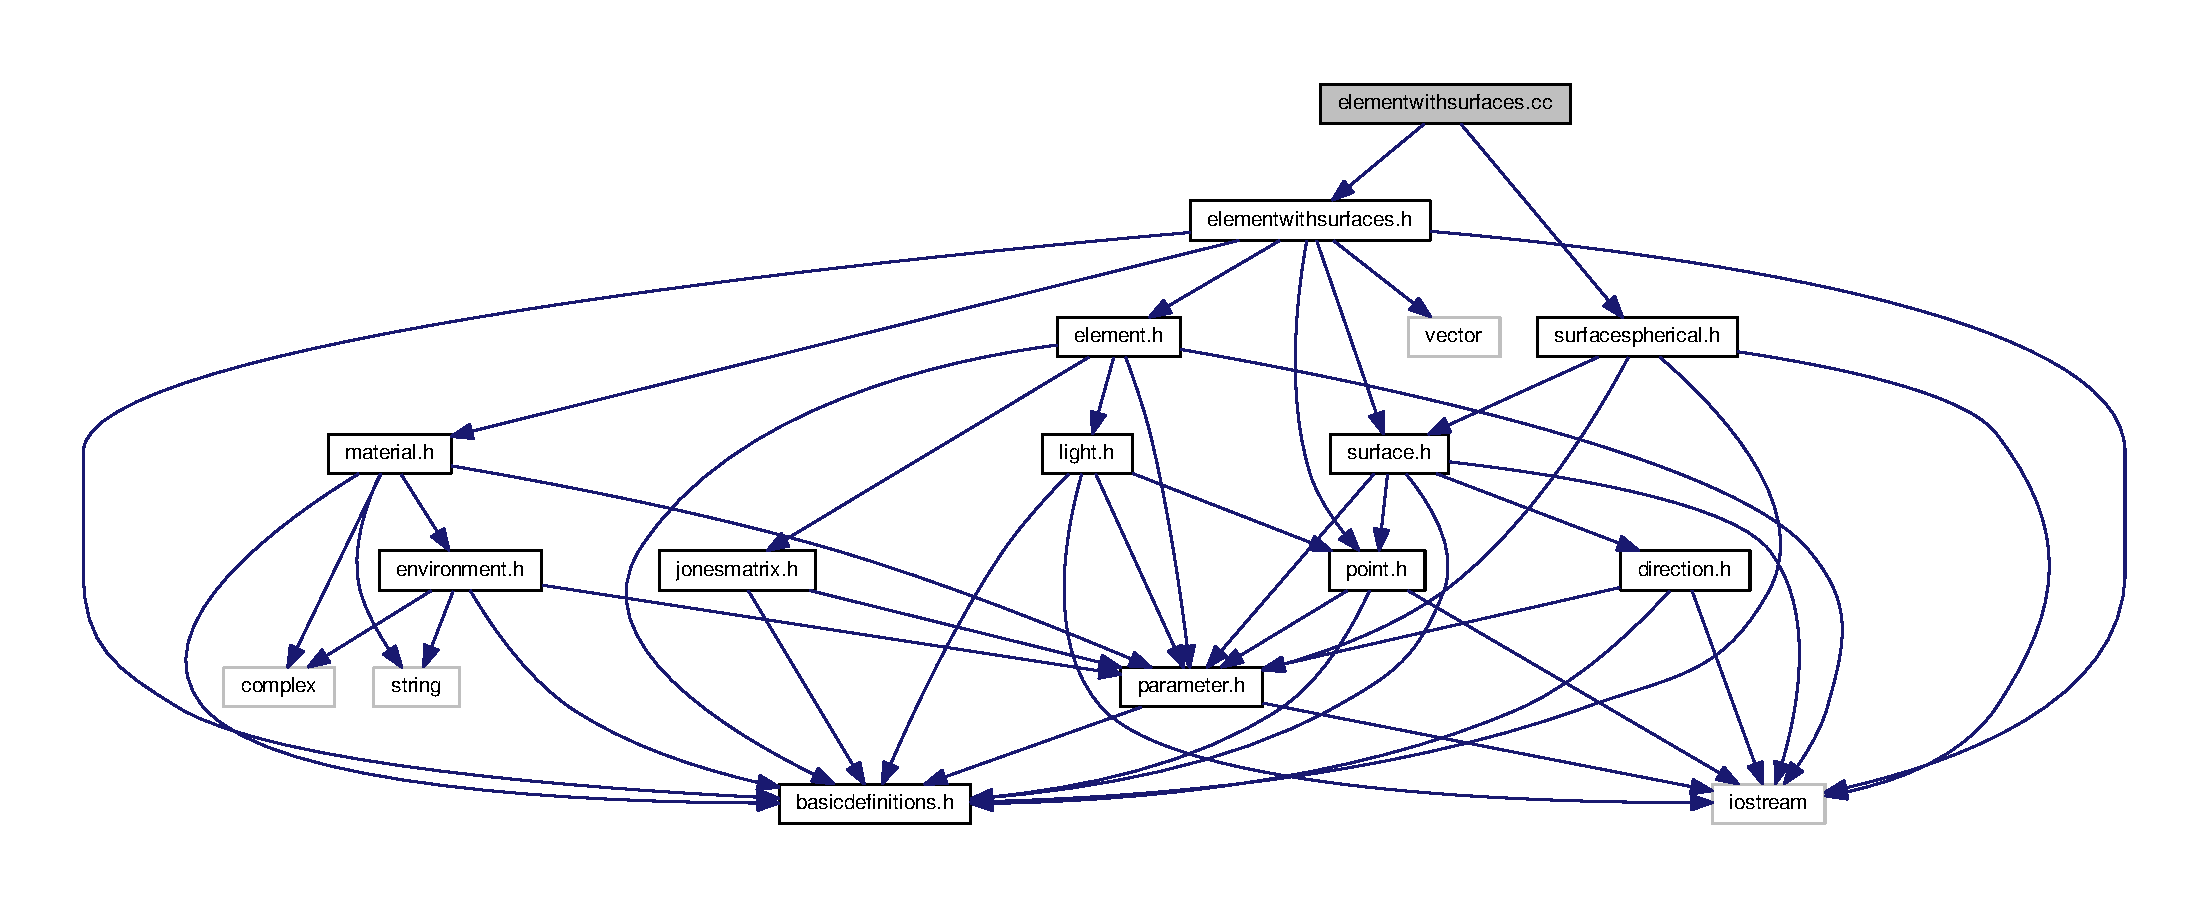
\includegraphics[width=350pt]{elementwithsurfaces_8cc__incl}
\end{center}
\end{figure}


\subsection{Detailed Description}
class \hyperlink{classElementWithSurfaces}{Element\+With\+Surfaces} 

\begin{DoxyDate}{Date}
15.\+04.\+2017 
\end{DoxyDate}
\begin{DoxyAuthor}{Author}
Tobias Haist (\href{mailto:haist@ito.uni-stuttgart.de}{\tt haist@ito.\+uni-\/stuttgart.\+de}) Institute of Applied Optics, University of Stuttgart I\+TO Paffenwaldring 9 70569 Stuttgart Germany 
\end{DoxyAuthor}

\hypertarget{elementwithsurfaces_8h}{}\section{elementwithsurfaces.\+h File Reference}
\label{elementwithsurfaces_8h}\index{elementwithsurfaces.\+h@{elementwithsurfaces.\+h}}


include file for class \hyperlink{classElementWithSurfaces}{Element\+With\+Surfaces}  


{\ttfamily \#include \char`\"{}basicdefinitions.\+h\char`\"{}}\\*
{\ttfamily \#include \char`\"{}element.\+h\char`\"{}}\\*
{\ttfamily \#include \char`\"{}surface.\+h\char`\"{}}\\*
{\ttfamily \#include \char`\"{}material.\+h\char`\"{}}\\*
{\ttfamily \#include \char`\"{}point.\+h\char`\"{}}\\*
{\ttfamily \#include $<$iostream$>$}\\*
{\ttfamily \#include $<$vector$>$}\\*
Include dependency graph for elementwithsurfaces.\+h\+:
\nopagebreak
\begin{figure}[H]
\begin{center}
\leavevmode
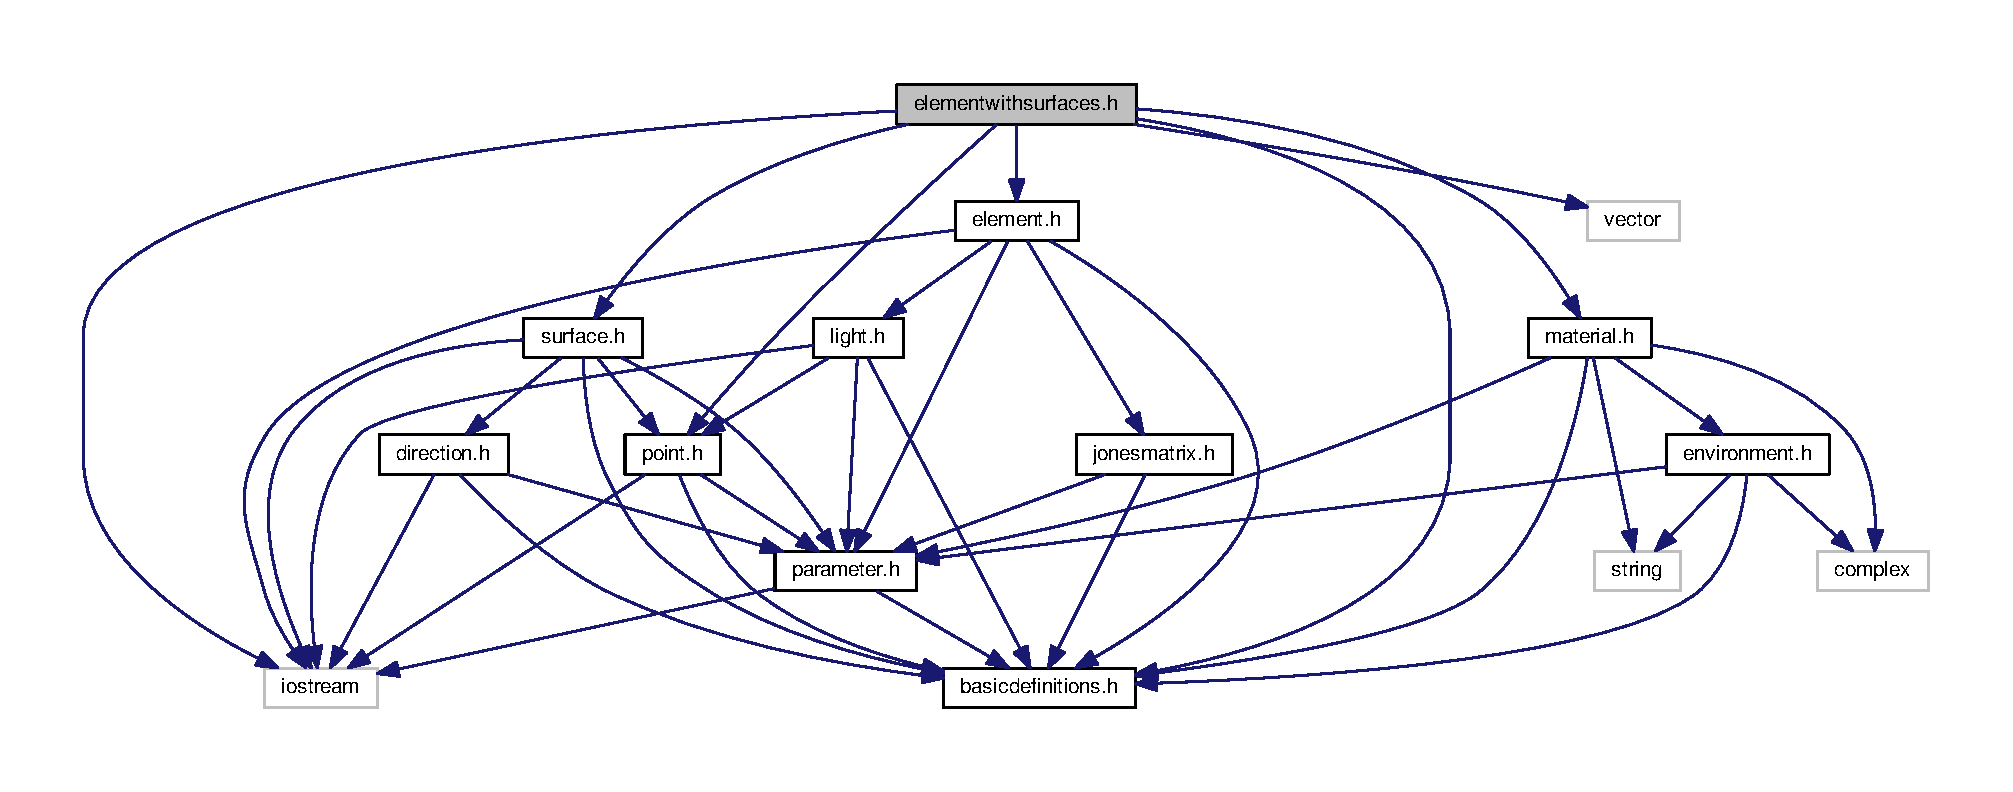
\includegraphics[width=350pt]{elementwithsurfaces_8h__incl}
\end{center}
\end{figure}
This graph shows which files directly or indirectly include this file\+:\nopagebreak
\begin{figure}[H]
\begin{center}
\leavevmode
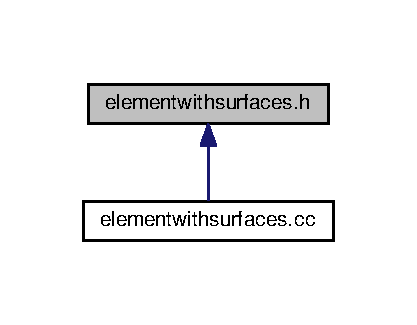
\includegraphics[width=200pt]{elementwithsurfaces_8h__dep__incl}
\end{center}
\end{figure}
\subsection*{Classes}
\begin{DoxyCompactItemize}
\item 
class \hyperlink{classElementWithSurfaces}{Element\+With\+Surfaces}
\begin{DoxyCompactList}\small\item\em \hyperlink{classElementWithSurfaces}{Element\+With\+Surfaces} represents things like typical lenses. \end{DoxyCompactList}\end{DoxyCompactItemize}


\subsection{Detailed Description}
include file for class \hyperlink{classElementWithSurfaces}{Element\+With\+Surfaces} 

\begin{DoxyDate}{Date}
07.\+04.\+2017 
\end{DoxyDate}
\begin{DoxyAuthor}{Author}
Tobias Haist (\href{mailto:haist@ito.uni-stuttgart.de}{\tt haist@ito.\+uni-\/stuttgart.\+de}) Institute of Applied Optics, University of Stuttgart I\+TO Paffenwaldring 9 70569 Stuttgart Germany 
\end{DoxyAuthor}

\hypertarget{environment_8cc}{}\section{environment.\+cc File Reference}
\label{environment_8cc}\index{environment.\+cc@{environment.\+cc}}


class \hyperlink{classEnvironment}{Environment}  


{\ttfamily \#include \char`\"{}material.\+h\char`\"{}}\\*
Include dependency graph for environment.\+cc\+:
\nopagebreak
\begin{figure}[H]
\begin{center}
\leavevmode
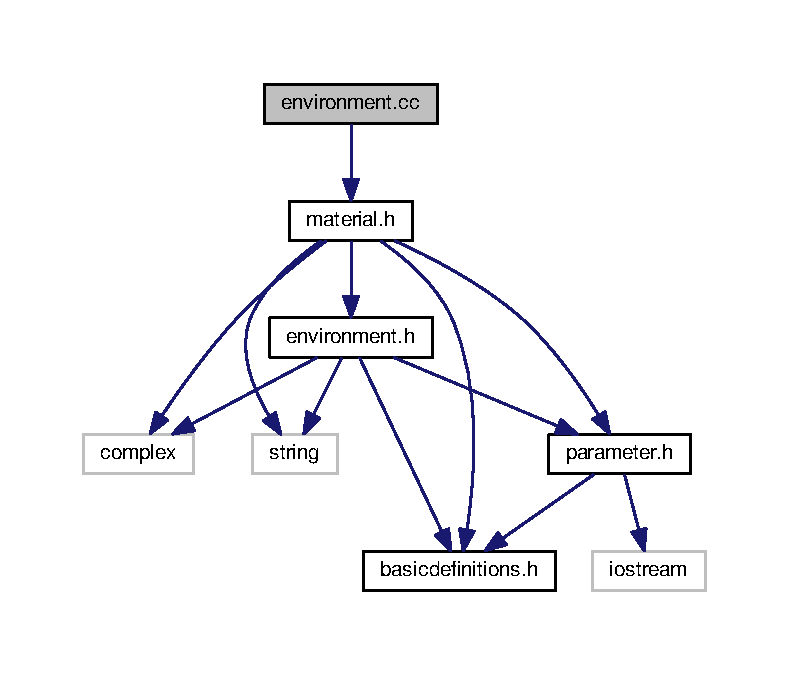
\includegraphics[width=350pt]{environment_8cc__incl}
\end{center}
\end{figure}


\subsection{Detailed Description}
class \hyperlink{classEnvironment}{Environment} 

\begin{DoxyDate}{Date}
15.\+04.\+2017 
\end{DoxyDate}
\begin{DoxyAuthor}{Author}
Tobias Haist (\href{mailto:haist@ito.uni-stuttgart.de}{\tt haist@ito.\+uni-\/stuttgart.\+de}) Institute of Applied Optics, University of Stuttgart I\+TO Paffenwaldring 9 70569 Stuttgart Germany 
\end{DoxyAuthor}

\hypertarget{interaction_8cc}{}\section{interaction.\+cc File Reference}
\label{interaction_8cc}\index{interaction.\+cc@{interaction.\+cc}}


class \hyperlink{classInteraction}{Interaction}  


{\ttfamily \#include \char`\"{}interaction.\+h\char`\"{}}\\*
{\ttfamily \#include \char`\"{}refractionrays.\+h\char`\"{}}\\*
{\ttfamily \#include \char`\"{}refractionwaves.\+h\char`\"{}}\\*
{\ttfamily \#include \char`\"{}traceopenerror.\+h\char`\"{}}\\*
Include dependency graph for interaction.\+cc\+:
\nopagebreak
\begin{figure}[H]
\begin{center}
\leavevmode
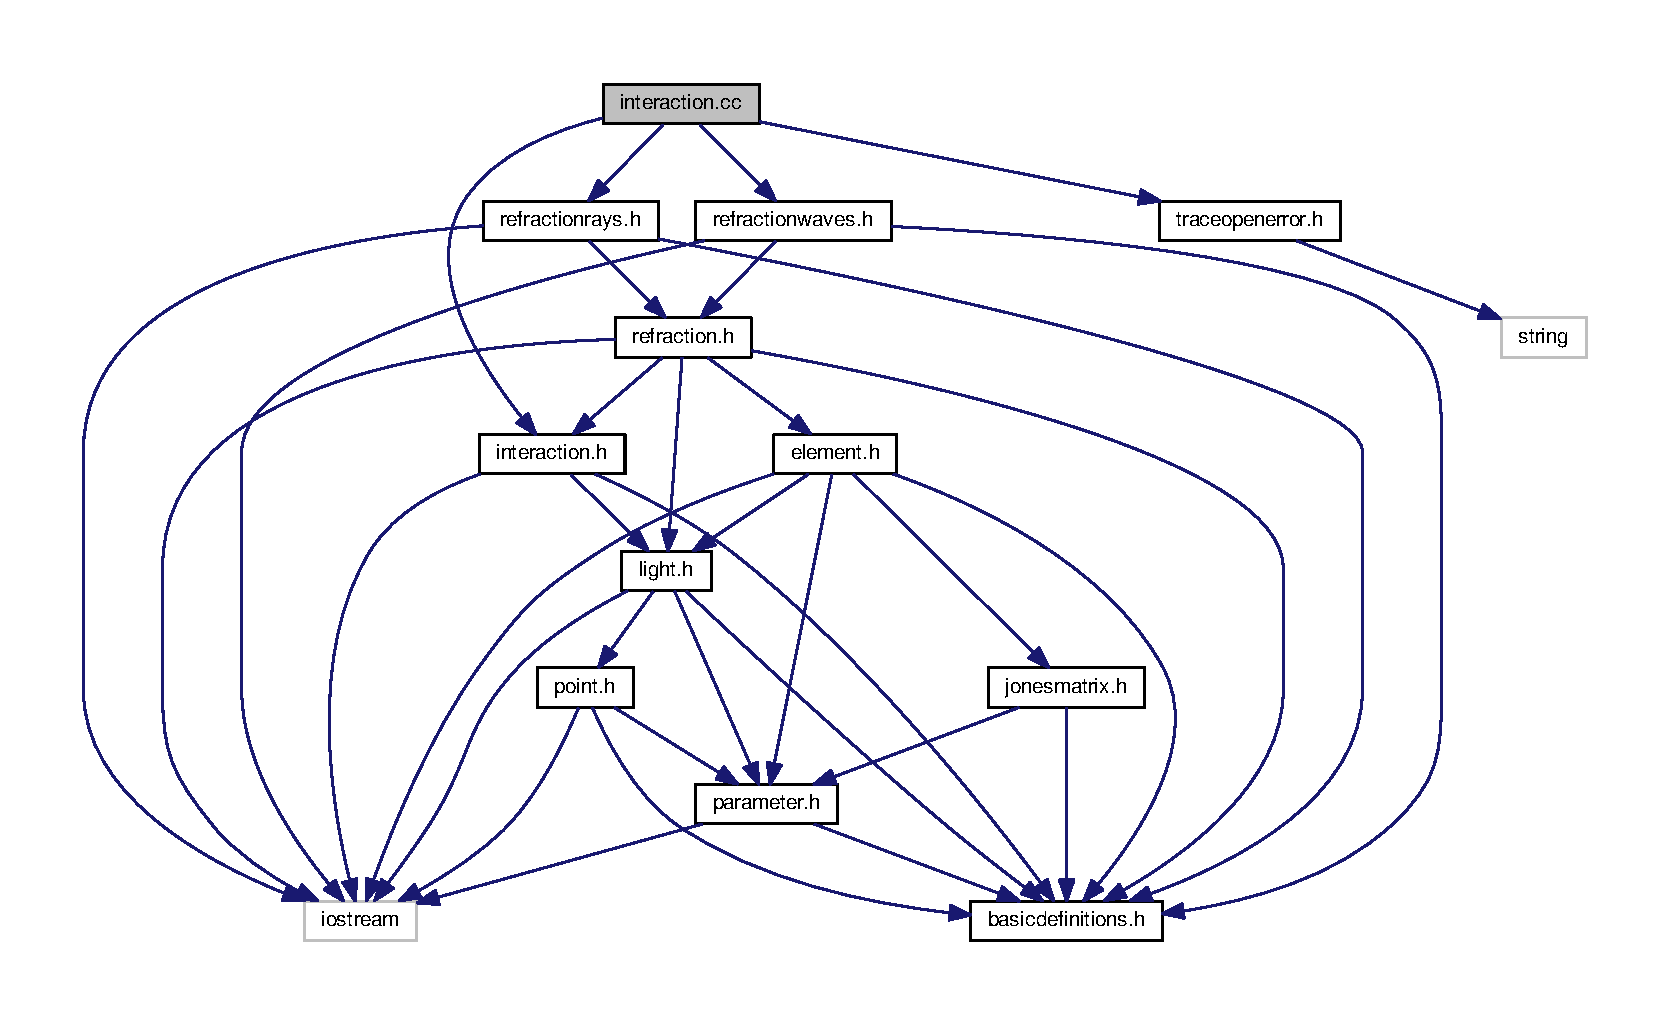
\includegraphics[width=350pt]{interaction_8cc__incl}
\end{center}
\end{figure}


\subsection{Detailed Description}
class \hyperlink{classInteraction}{Interaction} 

\begin{DoxyDate}{Date}
15.\+04.\+2017 
\end{DoxyDate}
\begin{DoxyAuthor}{Author}
Tobias Haist (\href{mailto:haist@ito.uni-stuttgart.de}{\tt haist@ito.\+uni-\/stuttgart.\+de}) Institute of Applied Optics, University of Stuttgart I\+TO Paffenwaldring 9 70569 Stuttgart Germany 
\end{DoxyAuthor}

\hypertarget{interaction_8h}{}\section{interaction.\+h File Reference}
\label{interaction_8h}\index{interaction.\+h@{interaction.\+h}}


include file for class \hyperlink{classInteraction}{Interaction}  


{\ttfamily \#include \char`\"{}basicdefinitions.\+h\char`\"{}}\\*
{\ttfamily \#include \char`\"{}light.\+h\char`\"{}}\\*
{\ttfamily \#include $<$iostream$>$}\\*
Include dependency graph for interaction.\+h\+:
\nopagebreak
\begin{figure}[H]
\begin{center}
\leavevmode
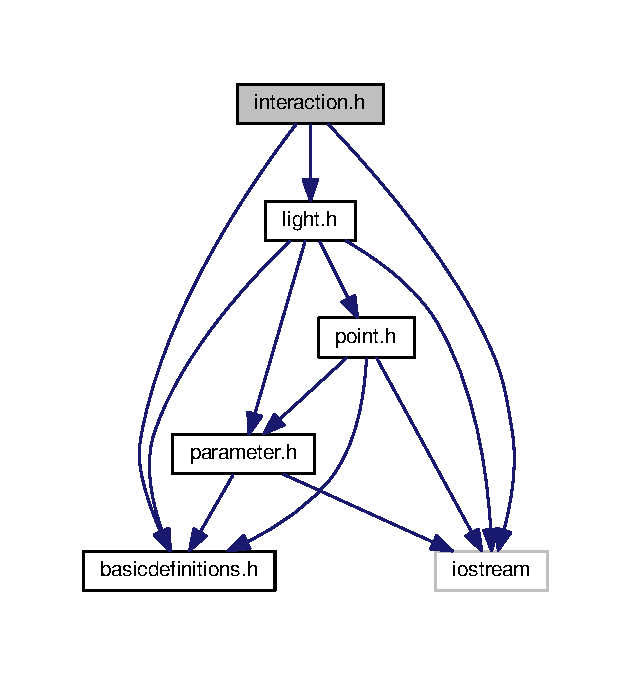
\includegraphics[width=303pt]{interaction_8h__incl}
\end{center}
\end{figure}
This graph shows which files directly or indirectly include this file\+:\nopagebreak
\begin{figure}[H]
\begin{center}
\leavevmode
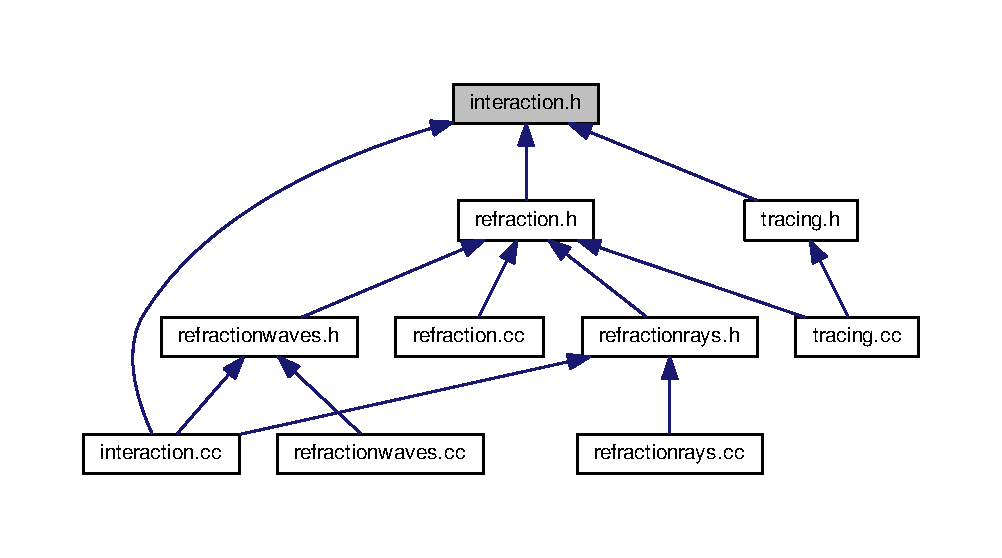
\includegraphics[width=350pt]{interaction_8h__dep__incl}
\end{center}
\end{figure}
\subsection*{Classes}
\begin{DoxyCompactItemize}
\item 
class \hyperlink{classInteraction}{Interaction}
\begin{DoxyCompactList}\small\item\em Most optical components are made out of Surfaces. \end{DoxyCompactList}\end{DoxyCompactItemize}


\subsection{Detailed Description}
include file for class \hyperlink{classInteraction}{Interaction} 

\begin{DoxyDate}{Date}
15.\+04.\+2017 
\end{DoxyDate}
\begin{DoxyAuthor}{Author}
Tobias Haist (\href{mailto:haist@ito.uni-stuttgart.de}{\tt haist@ito.\+uni-\/stuttgart.\+de}) Institute of Applied Optics, University of Stuttgart I\+TO Paffenwaldring 9 70569 Stuttgart Germany 
\end{DoxyAuthor}

\hypertarget{jonesmatrix_8cc}{}\section{jonesmatrix.\+cc File Reference}
\label{jonesmatrix_8cc}\index{jonesmatrix.\+cc@{jonesmatrix.\+cc}}


class \hyperlink{classJonesMatrix}{Jones\+Matrix}  


{\ttfamily \#include \char`\"{}jonesmatrix.\+h\char`\"{}}\\*
Include dependency graph for jonesmatrix.\+cc\+:
\nopagebreak
\begin{figure}[H]
\begin{center}
\leavevmode
\includegraphics[width=244pt]{jonesmatrix_8cc__incl}
\end{center}
\end{figure}


\subsection{Detailed Description}
class \hyperlink{classJonesMatrix}{Jones\+Matrix} 

\begin{DoxyDate}{Date}
15.\+04.\+2017 
\end{DoxyDate}
\begin{DoxyAuthor}{Author}
Tobias Haist (\href{mailto:haist@ito.uni-stuttgart.de}{\tt haist@ito.\+uni-\/stuttgart.\+de}) Institute of Applied Optics, University of Stuttgart I\+TO Paffenwaldring 9 70569 Stuttgart Germany 
\end{DoxyAuthor}

\hypertarget{jonesmatrix_8h}{}\section{jonesmatrix.\+h File Reference}
\label{jonesmatrix_8h}\index{jonesmatrix.\+h@{jonesmatrix.\+h}}


include file for class \hyperlink{classJonesMatrix}{Jones\+Matrix}  


{\ttfamily \#include \char`\"{}basicdefinitions.\+h\char`\"{}}\\*
{\ttfamily \#include \char`\"{}parameter.\+h\char`\"{}}\\*
Include dependency graph for jonesmatrix.\+h\+:
\nopagebreak
\begin{figure}[H]
\begin{center}
\leavevmode
\includegraphics[width=244pt]{jonesmatrix_8h__incl}
\end{center}
\end{figure}
This graph shows which files directly or indirectly include this file\+:
\nopagebreak
\begin{figure}[H]
\begin{center}
\leavevmode
\includegraphics[width=350pt]{jonesmatrix_8h__dep__incl}
\end{center}
\end{figure}
\subsection*{Classes}
\begin{DoxyCompactItemize}
\item 
class \hyperlink{classJonesMatrix}{Jones\+Matrix}
\begin{DoxyCompactList}\small\item\em \hyperlink{classJonesMatrix}{Jones\+Matrix} is just the Jones matrix of an element. \end{DoxyCompactList}\end{DoxyCompactItemize}


\subsection{Detailed Description}
include file for class \hyperlink{classJonesMatrix}{Jones\+Matrix} 

\begin{DoxyDate}{Date}
07.\+04.\+2017 
\end{DoxyDate}
\begin{DoxyAuthor}{Author}
Tobias Haist (\href{mailto:haist@ito.uni-stuttgart.de}{\tt haist@ito.\+uni-\/stuttgart.\+de}) Institute of Applied Optics, University of Stuttgart I\+TO Paffenwaldring 9 70569 Stuttgart Germany 
\end{DoxyAuthor}

\hypertarget{light_8cc}{}\section{light.\+cc File Reference}
\label{light_8cc}\index{light.\+cc@{light.\+cc}}


class \hyperlink{classElement}{Element}  


{\ttfamily \#include \char`\"{}light.\+h\char`\"{}}\\*
Include dependency graph for light.\+cc\+:
\nopagebreak
\begin{figure}[H]
\begin{center}
\leavevmode
\includegraphics[width=271pt]{light_8cc__incl}
\end{center}
\end{figure}


\subsection{Detailed Description}
class \hyperlink{classElement}{Element} 

\begin{DoxyDate}{Date}
07.\+04.\+2017 
\end{DoxyDate}
\begin{DoxyAuthor}{Author}
Tobias Haist (\href{mailto:haist@ito.uni-stuttgart.de}{\tt haist@ito.\+uni-\/stuttgart.\+de}) Institute of Applied Optics, University of Stuttgart I\+TO Paffenwaldring 9 70569 Stuttgart Germany 
\end{DoxyAuthor}

\hypertarget{light_8h}{}\section{light.\+h File Reference}
\label{light_8h}\index{light.\+h@{light.\+h}}


include file for class \hyperlink{classLight}{Light}  


{\ttfamily \#include \char`\"{}basicdefinitions.\+h\char`\"{}}\\*
{\ttfamily \#include \char`\"{}parameter.\+h\char`\"{}}\\*
{\ttfamily \#include \char`\"{}point.\+h\char`\"{}}\\*
{\ttfamily \#include $<$iostream$>$}\\*
Include dependency graph for light.\+h\+:
\nopagebreak
\begin{figure}[H]
\begin{center}
\leavevmode
\includegraphics[width=271pt]{light_8h__incl}
\end{center}
\end{figure}
This graph shows which files directly or indirectly include this file\+:\nopagebreak
\begin{figure}[H]
\begin{center}
\leavevmode
\includegraphics[width=350pt]{light_8h__dep__incl}
\end{center}
\end{figure}
\subsection*{Classes}
\begin{DoxyCompactItemize}
\item 
class \hyperlink{classLight}{Light}
\end{DoxyCompactItemize}
\subsection*{Enumerations}
\begin{DoxyCompactItemize}
\item 
enum \hyperlink{light_8h_a6dc57eac1ae8b19466de554123d5c6c3}{type\+Light} \{ {\bfseries type\+Light\+Ray}, 
{\bfseries type\+Wave\+Scalar}, 
{\bfseries type\+Wave\+Vectorial}, 
{\bfseries type\+Gaussian}
 \}\begin{DoxyCompactList}\small\item\em The abstract class light is the base class for all our light models. \end{DoxyCompactList}
\end{DoxyCompactItemize}


\subsection{Detailed Description}
include file for class \hyperlink{classLight}{Light} 

\begin{DoxyDate}{Date}
07.\+04.\+2017 
\end{DoxyDate}
\begin{DoxyAuthor}{Author}
Tobias Haist (\href{mailto:haist@ito.uni-stuttgart.de}{\tt haist@ito.\+uni-\/stuttgart.\+de}) Institute of Applied Optics, University of Stuttgart I\+TO Paffenwaldring 9 70569 Stuttgart Germany 
\end{DoxyAuthor}


\subsection{Enumeration Type Documentation}
\index{light.\+h@{light.\+h}!type\+Light@{type\+Light}}
\index{type\+Light@{type\+Light}!light.\+h@{light.\+h}}
\subsubsection[{\texorpdfstring{type\+Light}{typeLight}}]{\setlength{\rightskip}{0pt plus 5cm}enum {\bf type\+Light}}\hypertarget{light_8h_a6dc57eac1ae8b19466de554123d5c6c3}{}\label{light_8h_a6dc57eac1ae8b19466de554123d5c6c3}


The abstract class light is the base class for all our light models. 

Different models of light are used in optics. Most often, optical design can be successfully achieved using the geometrical model based on rays. However, for some applications we want to be able to use completely different models. It is obvious that sometimes some sort of wave optics (scalar or vectorial) is necessary. Even for these, different formulations are possible. In addition, sometimes even more uncommen approaches (e.\+g. path integrals) are feasible.

Up till now, we only implement ray-\/based simulations. But Traceopen should be easily extensible to other light models. This is why the whole structure is already prepared to handle other models. \char`\"{}\+Light\char`\"{} is the base class for our light models. The class \char`\"{}\+Ray\char`\"{} e.\+g. is derived from \hyperlink{classLight}{Light}.

\begin{DoxyDate}{Date}
07.\+4.\+2017 
\end{DoxyDate}
\begin{DoxyAuthor}{Author}
Tobias Haist (\href{mailto:haist@ito.uni-stuttgart.de}{\tt haist@ito.\+uni-\/stuttgart.\+de}) 
\end{DoxyAuthor}

\hypertarget{material_8cc}{}\section{material.\+cc File Reference}
\label{material_8cc}\index{material.\+cc@{material.\+cc}}


class \hyperlink{classMaterial}{Material} (abstract base class)  


{\ttfamily \#include \char`\"{}material.\+h\char`\"{}}\\*
Include dependency graph for material.\+cc\+:
\nopagebreak
\begin{figure}[H]
\begin{center}
\leavevmode
\includegraphics[width=350pt]{material_8cc__incl}
\end{center}
\end{figure}


\subsection{Detailed Description}
class \hyperlink{classMaterial}{Material} (abstract base class) 

\begin{DoxyDate}{Date}
15.\+04.\+2017 
\end{DoxyDate}
\begin{DoxyAuthor}{Author}
Tobias Haist (\href{mailto:haist@ito.uni-stuttgart.de}{\tt haist@ito.\+uni-\/stuttgart.\+de}) Institute of Applied Optics, University of Stuttgart I\+TO Paffenwaldring 9 70569 Stuttgart Germany 
\end{DoxyAuthor}

\hypertarget{material_8h}{}\section{material.\+h File Reference}
\label{material_8h}\index{material.\+h@{material.\+h}}


include file for class \hyperlink{classMaterial}{Material}  


{\ttfamily \#include $<$complex$>$}\\*
{\ttfamily \#include $<$string$>$}\\*
{\ttfamily \#include \char`\"{}basicdefinitions.\+h\char`\"{}}\\*
{\ttfamily \#include \char`\"{}parameter.\+h\char`\"{}}\\*
{\ttfamily \#include \char`\"{}environment.\+h\char`\"{}}\\*
Include dependency graph for material.\+h\+:
\nopagebreak
\begin{figure}[H]
\begin{center}
\leavevmode
\includegraphics[width=350pt]{material_8h__incl}
\end{center}
\end{figure}
This graph shows which files directly or indirectly include this file\+:
\nopagebreak
\begin{figure}[H]
\begin{center}
\leavevmode
\includegraphics[width=350pt]{material_8h__dep__incl}
\end{center}
\end{figure}
\subsection*{Classes}
\begin{DoxyCompactItemize}
\item 
class \hyperlink{classMaterial}{Material}
\begin{DoxyCompactList}\small\item\em \hyperlink{classMaterial}{Material} is an abstract base calls that represents all Materials. \end{DoxyCompactList}\end{DoxyCompactItemize}


\subsection{Detailed Description}
include file for class \hyperlink{classMaterial}{Material} 

\begin{DoxyDate}{Date}
07.\+04.\+2017 
\end{DoxyDate}
\begin{DoxyAuthor}{Author}
Tobias Haist (\href{mailto:haist@ito.uni-stuttgart.de}{\tt haist@ito.\+uni-\/stuttgart.\+de}) Institute of Applied Optics, University of Stuttgart I\+TO Paffenwaldring 9 70569 Stuttgart Germany 
\end{DoxyAuthor}

\hypertarget{materialideal_8h}{}\section{materialideal.\+h File Reference}
\label{materialideal_8h}\index{materialideal.\+h@{materialideal.\+h}}


include file for class \hyperlink{classMaterialIdeal}{Material\+Ideal}  


{\ttfamily \#include $<$complex$>$}\\*
{\ttfamily \#include \char`\"{}basicdefinitions.\+h\char`\"{}}\\*
{\ttfamily \#include \char`\"{}parameter.\+h\char`\"{}}\\*
{\ttfamily \#include \char`\"{}environment.\+h\char`\"{}}\\*
{\ttfamily \#include \char`\"{}material.\+h\char`\"{}}\\*
Include dependency graph for materialideal.\+h\+:
\nopagebreak
\begin{figure}[H]
\begin{center}
\leavevmode
\includegraphics[width=350pt]{materialideal_8h__incl}
\end{center}
\end{figure}
\subsection*{Classes}
\begin{DoxyCompactItemize}
\item 
class \hyperlink{classMaterialIdeal}{Material\+Ideal}
\begin{DoxyCompactList}\small\item\em \hyperlink{classMaterialIdeal}{Material\+Ideal} represents all ideal Materials. \end{DoxyCompactList}\end{DoxyCompactItemize}


\subsection{Detailed Description}
include file for class \hyperlink{classMaterialIdeal}{Material\+Ideal} 

\begin{DoxyDate}{Date}
07.\+04.\+2017 
\end{DoxyDate}
\begin{DoxyAuthor}{Author}
Tobias Haist (\href{mailto:haist@ito.uni-stuttgart.de}{\tt haist@ito.\+uni-\/stuttgart.\+de}) Institute of Applied Optics, University of Stuttgart I\+TO Paffenwaldring 9 70569 Stuttgart Germany 
\end{DoxyAuthor}

\hypertarget{opticalsystem_8cc}{}\section{opticalsystem.\+cc File Reference}
\label{opticalsystem_8cc}\index{opticalsystem.\+cc@{opticalsystem.\+cc}}


class \hyperlink{classOpticalSystem}{Optical\+System}  


{\ttfamily \#include \char`\"{}opticalsystem.\+h\char`\"{}}\\*
Include dependency graph for opticalsystem.\+cc\+:
\nopagebreak
\begin{figure}[H]
\begin{center}
\leavevmode
\includegraphics[width=350pt]{opticalsystem_8cc__incl}
\end{center}
\end{figure}


\subsection{Detailed Description}
class \hyperlink{classOpticalSystem}{Optical\+System} 

\begin{DoxyDate}{Date}
15.\+04.\+2017 
\end{DoxyDate}
\begin{DoxyAuthor}{Author}
Tobias Haist (\href{mailto:haist@ito.uni-stuttgart.de}{\tt haist@ito.\+uni-\/stuttgart.\+de}) Institute of Applied Optics, University of Stuttgart I\+TO Paffenwaldring 9 70569 Stuttgart Germany 
\end{DoxyAuthor}

\hypertarget{opticalsystem_8h}{}\section{opticalsystem.\+h File Reference}
\label{opticalsystem_8h}\index{opticalsystem.\+h@{opticalsystem.\+h}}


include file for class \hyperlink{classSurface}{Surface}  


{\ttfamily \#include \char`\"{}basicdefinitions.\+h\char`\"{}}\\*
{\ttfamily \#include \char`\"{}element.\+h\char`\"{}}\\*
{\ttfamily \#include \char`\"{}parameter.\+h\char`\"{}}\\*
{\ttfamily \#include \char`\"{}surface.\+h\char`\"{}}\\*
{\ttfamily \#include $<$vector$>$}\\*
{\ttfamily \#include $<$iostream$>$}\\*
Include dependency graph for opticalsystem.\+h\+:
\nopagebreak
\begin{figure}[H]
\begin{center}
\leavevmode
\includegraphics[width=350pt]{opticalsystem_8h__incl}
\end{center}
\end{figure}
This graph shows which files directly or indirectly include this file\+:\nopagebreak
\begin{figure}[H]
\begin{center}
\leavevmode
\includegraphics[width=331pt]{opticalsystem_8h__dep__incl}
\end{center}
\end{figure}
\subsection*{Classes}
\begin{DoxyCompactItemize}
\item 
class \hyperlink{classOpticalSystem}{Optical\+System}
\begin{DoxyCompactList}\small\item\em Describes the complete optical system. \end{DoxyCompactList}\end{DoxyCompactItemize}


\subsection{Detailed Description}
include file for class \hyperlink{classSurface}{Surface} 

\begin{DoxyDate}{Date}
07.\+04.\+2017 
\end{DoxyDate}
\begin{DoxyAuthor}{Author}
Tobias Haist (\href{mailto:haist@ito.uni-stuttgart.de}{\tt haist@ito.\+uni-\/stuttgart.\+de}) Institute of Applied Optics, University of Stuttgart I\+TO Paffenwaldring 9 70569 Stuttgart Germany 
\end{DoxyAuthor}

\hypertarget{parameter_8h}{}\section{parameter.\+h File Reference}
\label{parameter_8h}\index{parameter.\+h@{parameter.\+h}}


include file for class \hyperlink{classParameter}{Parameter}  


{\ttfamily \#include \char`\"{}basicdefinitions.\+h\char`\"{}}\\*
{\ttfamily \#include $<$iostream$>$}\\*
Include dependency graph for parameter.\+h\+:\nopagebreak
\begin{figure}[H]
\begin{center}
\leavevmode
\includegraphics[width=244pt]{parameter_8h__incl}
\end{center}
\end{figure}
This graph shows which files directly or indirectly include this file\+:
\nopagebreak
\begin{figure}[H]
\begin{center}
\leavevmode
\includegraphics[width=350pt]{parameter_8h__dep__incl}
\end{center}
\end{figure}
\subsection*{Classes}
\begin{DoxyCompactItemize}
\item 
class \hyperlink{classParameter}{Parameter$<$ Type $>$}
\begin{DoxyCompactList}\small\item\em \hyperlink{classParameter}{Parameter} manages changeable Parameters (e.\+g. for optimization) \end{DoxyCompactList}\end{DoxyCompactItemize}
\subsection*{Enumerations}
\begin{DoxyCompactItemize}
\item 
enum {\bfseries type\+Modifier} \{ {\bfseries type\+Modifier\+Fixed}, 
{\bfseries type\+Modifier\+Variable}, 
{\bfseries type\+Modifier\+Pickup}
 \}\hypertarget{parameter_8h_a494a3e6306855e56450d700f067f115e}{}\label{parameter_8h_a494a3e6306855e56450d700f067f115e}

\end{DoxyCompactItemize}


\subsection{Detailed Description}
include file for class \hyperlink{classParameter}{Parameter} 

\begin{DoxyDate}{Date}
07.\+04.\+2017 
\end{DoxyDate}
\begin{DoxyAuthor}{Author}
Tobias Haist (\href{mailto:haist@ito.uni-stuttgart.de}{\tt haist@ito.\+uni-\/stuttgart.\+de}) Institute of Applied Optics, University of Stuttgart I\+TO Paffenwaldring 9 70569 Stuttgart Germany 
\end{DoxyAuthor}

\hypertarget{point_8cc}{}\section{point.\+cc File Reference}
\label{point_8cc}\index{point.\+cc@{point.\+cc}}


class \hyperlink{classPoint}{Point}  


{\ttfamily \#include \char`\"{}point.\+h\char`\"{}}\\*
Include dependency graph for point.\+cc\+:
\nopagebreak
\begin{figure}[H]
\begin{center}
\leavevmode
\includegraphics[width=260pt]{point_8cc__incl}
\end{center}
\end{figure}


\subsection{Detailed Description}
class \hyperlink{classPoint}{Point} 

\begin{DoxyDate}{Date}
15.\+04.\+2017 
\end{DoxyDate}
\begin{DoxyAuthor}{Author}
Tobias Haist (\href{mailto:haist@ito.uni-stuttgart.de}{\tt haist@ito.\+uni-\/stuttgart.\+de}) Institute of Applied Optics, University of Stuttgart I\+TO Paffenwaldring 9 70569 Stuttgart Germany 
\end{DoxyAuthor}

\hypertarget{point_8h}{}\section{point.\+h File Reference}
\label{point_8h}\index{point.\+h@{point.\+h}}


include file for class \hyperlink{classPoint}{Point}  


{\ttfamily \#include \char`\"{}basicdefinitions.\+h\char`\"{}}\\*
{\ttfamily \#include \char`\"{}parameter.\+h\char`\"{}}\\*
{\ttfamily \#include $<$iostream$>$}\\*
Include dependency graph for point.\+h\+:
\nopagebreak
\begin{figure}[H]
\begin{center}
\leavevmode
\includegraphics[width=260pt]{point_8h__incl}
\end{center}
\end{figure}
This graph shows which files directly or indirectly include this file\+:\nopagebreak
\begin{figure}[H]
\begin{center}
\leavevmode
\includegraphics[width=350pt]{point_8h__dep__incl}
\end{center}
\end{figure}
\subsection*{Classes}
\begin{DoxyCompactItemize}
\item 
class \hyperlink{classPoint}{Point}
\begin{DoxyCompactList}\small\item\em \hyperlink{classPoint}{Point} manages Points/\+Positions in Space. \end{DoxyCompactList}\end{DoxyCompactItemize}


\subsection{Detailed Description}
include file for class \hyperlink{classPoint}{Point} 

\begin{DoxyDate}{Date}
07.\+04.\+2017 
\end{DoxyDate}
\begin{DoxyAuthor}{Author}
Tobias Haist (\href{mailto:haist@ito.uni-stuttgart.de}{\tt haist@ito.\+uni-\/stuttgart.\+de}) Institute of Applied Optics, University of Stuttgart I\+TO Paffenwaldring 9 70569 Stuttgart Germany 
\end{DoxyAuthor}

\hypertarget{ray_8cc}{}\section{ray.\+cc File Reference}
\label{ray_8cc}\index{ray.\+cc@{ray.\+cc}}


class \hyperlink{classRay}{Ray}  


{\ttfamily \#include \char`\"{}ray.\+h\char`\"{}}\\*
{\ttfamily \#include \char`\"{}logging.\+h\char`\"{}}\\*
Include dependency graph for ray.\+cc\+:
\nopagebreak
\begin{figure}[H]
\begin{center}
\leavevmode
\includegraphics[width=350pt]{ray_8cc__incl}
\end{center}
\end{figure}


\subsection{Detailed Description}
class \hyperlink{classRay}{Ray} 

\begin{DoxyDate}{Date}
07.\+04.\+2017 
\end{DoxyDate}
\begin{DoxyAuthor}{Author}
Tobias Haist (\href{mailto:haist@ito.uni-stuttgart.de}{\tt haist@ito.\+uni-\/stuttgart.\+de}) Institute of Applied Optics, University of Stuttgart I\+TO Paffenwaldring 9 70569 Stuttgart Germany 
\end{DoxyAuthor}

\hypertarget{ray_8h}{}\section{ray.\+h File Reference}
\label{ray_8h}\index{ray.\+h@{ray.\+h}}


include file for class \hyperlink{classRay}{Ray}  


{\ttfamily \#include \char`\"{}basicdefinitions.\+h\char`\"{}}\\*
{\ttfamily \#include \char`\"{}point.\+h\char`\"{}}\\*
{\ttfamily \#include \char`\"{}direction.\+h\char`\"{}}\\*
{\ttfamily \#include \char`\"{}light.\+h\char`\"{}}\\*
{\ttfamily \#include $<$iostream$>$}\\*
Include dependency graph for ray.\+h\+:
\nopagebreak
\begin{figure}[H]
\begin{center}
\leavevmode
\includegraphics[width=350pt]{ray_8h__incl}
\end{center}
\end{figure}
This graph shows which files directly or indirectly include this file\+:\nopagebreak
\begin{figure}[H]
\begin{center}
\leavevmode
\includegraphics[width=124pt]{ray_8h__dep__incl}
\end{center}
\end{figure}
\subsection*{Classes}
\begin{DoxyCompactItemize}
\item 
class \hyperlink{classRay}{Ray}
\begin{DoxyCompactList}\small\item\em \hyperlink{classRay}{Ray} manages optical (polarized or unpolarized) Rays. \end{DoxyCompactList}\end{DoxyCompactItemize}


\subsection{Detailed Description}
include file for class \hyperlink{classRay}{Ray} 

\begin{DoxyDate}{Date}
07.\+04.\+2017 
\end{DoxyDate}
\begin{DoxyAuthor}{Author}
Tobias Haist (\href{mailto:haist@ito.uni-stuttgart.de}{\tt haist@ito.\+uni-\/stuttgart.\+de}) Institute of Applied Optics, University of Stuttgart I\+TO Paffenwaldring 9 70569 Stuttgart Germany 
\end{DoxyAuthor}

\hypertarget{rayaiming_8h}{}\section{rayaiming.\+h File Reference}
\label{rayaiming_8h}\index{rayaiming.\+h@{rayaiming.\+h}}


include file for class \hyperlink{classRayAiming}{Ray\+Aiming}  


{\ttfamily \#include \char`\"{}basicdefinitions.\+h\char`\"{}}\\*
{\ttfamily \#include \char`\"{}light.\+h\char`\"{}}\\*
{\ttfamily \#include \char`\"{}opticalsystem.\+h\char`\"{}}\\*
{\ttfamily \#include $<$iostream$>$}\\*
Include dependency graph for rayaiming.\+h\+:
\nopagebreak
\begin{figure}[H]
\begin{center}
\leavevmode
\includegraphics[width=350pt]{rayaiming_8h__incl}
\end{center}
\end{figure}
\subsection*{Classes}
\begin{DoxyCompactItemize}
\item 
class \hyperlink{classRayAiming}{Ray\+Aiming}
\begin{DoxyCompactList}\small\item\em \hyperlink{classRayAiming}{Ray\+Aiming} implements rayaiming \+:) \end{DoxyCompactList}\end{DoxyCompactItemize}


\subsection{Detailed Description}
include file for class \hyperlink{classRayAiming}{Ray\+Aiming} 

\begin{DoxyDate}{Date}
07.\+04.\+2017 
\end{DoxyDate}
\begin{DoxyAuthor}{Author}
Tobias Haist (\href{mailto:haist@ito.uni-stuttgart.de}{\tt haist@ito.\+uni-\/stuttgart.\+de}) Institute of Applied Optics, University of Stuttgart I\+TO 1999 Paffenwaldring 9 70569 Stuttgart Germany 
\end{DoxyAuthor}

\hypertarget{refraction_8cc}{}\section{refraction.\+cc File Reference}
\label{refraction_8cc}\index{refraction.\+cc@{refraction.\+cc}}


class \hyperlink{classRefraction}{Refraction}  


{\ttfamily \#include \char`\"{}refraction.\+h\char`\"{}}\\*
Include dependency graph for refraction.\+cc\+:
\nopagebreak
\begin{figure}[H]
\begin{center}
\leavevmode
\includegraphics[width=350pt]{refraction_8cc__incl}
\end{center}
\end{figure}


\subsection{Detailed Description}
class \hyperlink{classRefraction}{Refraction} 

\begin{DoxyDate}{Date}
15.\+04.\+2017 
\end{DoxyDate}
\begin{DoxyAuthor}{Author}
Tobias Haist (\href{mailto:haist@ito.uni-stuttgart.de}{\tt haist@ito.\+uni-\/stuttgart.\+de}) Institute of Applied Optics, University of Stuttgart I\+TO Paffenwaldring 9 70569 Stuttgart Germany 
\end{DoxyAuthor}

\hypertarget{refraction_8h}{}\section{refraction.\+h File Reference}
\label{refraction_8h}\index{refraction.\+h@{refraction.\+h}}


include file for class \hyperlink{classInteraction}{Interaction}  


{\ttfamily \#include \char`\"{}basicdefinitions.\+h\char`\"{}}\\*
{\ttfamily \#include \char`\"{}light.\+h\char`\"{}}\\*
{\ttfamily \#include \char`\"{}interaction.\+h\char`\"{}}\\*
{\ttfamily \#include \char`\"{}element.\+h\char`\"{}}\\*
{\ttfamily \#include $<$iostream$>$}\\*
Include dependency graph for refraction.\+h\+:
\nopagebreak
\begin{figure}[H]
\begin{center}
\leavevmode
\includegraphics[width=350pt]{refraction_8h__incl}
\end{center}
\end{figure}
This graph shows which files directly or indirectly include this file\+:\nopagebreak
\begin{figure}[H]
\begin{center}
\leavevmode
\includegraphics[width=350pt]{refraction_8h__dep__incl}
\end{center}
\end{figure}
\subsection*{Classes}
\begin{DoxyCompactItemize}
\item 
class \hyperlink{classRefraction}{Refraction}
\begin{DoxyCompactList}\small\item\em Most optical components are made out of Surfaces. \end{DoxyCompactList}\end{DoxyCompactItemize}


\subsection{Detailed Description}
include file for class \hyperlink{classInteraction}{Interaction} 

\begin{DoxyDate}{Date}
15.\+04.\+2017 
\end{DoxyDate}
\begin{DoxyAuthor}{Author}
Tobias Haist (\href{mailto:haist@ito.uni-stuttgart.de}{\tt haist@ito.\+uni-\/stuttgart.\+de}) Institute of Applied Optics, University of Stuttgart I\+TO Paffenwaldring 9 70569 Stuttgart Germany 
\end{DoxyAuthor}

\hypertarget{refractionrays_8cc}{}\section{refractionrays.\+cc File Reference}
\label{refractionrays_8cc}\index{refractionrays.\+cc@{refractionrays.\+cc}}


class \hyperlink{classRefractionRays}{Refraction\+Rays}  


{\ttfamily \#include \char`\"{}refractionrays.\+h\char`\"{}}\\*
{\ttfamily \#include \char`\"{}traceopenerror.\+h\char`\"{}}\\*
{\ttfamily \#include $<$iostream$>$}\\*
{\ttfamily \#include \char`\"{}logging.\+h\char`\"{}}\\*
Include dependency graph for refractionrays.\+cc\+:
\nopagebreak
\begin{figure}[H]
\begin{center}
\leavevmode
\includegraphics[width=350pt]{refractionrays_8cc__incl}
\end{center}
\end{figure}


\subsection{Detailed Description}
class \hyperlink{classRefractionRays}{Refraction\+Rays} 

\begin{DoxyDate}{Date}
15.\+04.\+2017 
\end{DoxyDate}
\begin{DoxyAuthor}{Author}
Tobias Haist (\href{mailto:haist@ito.uni-stuttgart.de}{\tt haist@ito.\+uni-\/stuttgart.\+de}) Institute of Applied Optics, University of Stuttgart I\+TO Paffenwaldring 9 70569 Stuttgart Germany 
\end{DoxyAuthor}

\hypertarget{refractionrays_8h}{}\section{refractionrays.\+h File Reference}
\label{refractionrays_8h}\index{refractionrays.\+h@{refractionrays.\+h}}


include file for class \hyperlink{classInteraction}{Interaction}  


{\ttfamily \#include \char`\"{}basicdefinitions.\+h\char`\"{}}\\*
{\ttfamily \#include \char`\"{}refraction.\+h\char`\"{}}\\*
{\ttfamily \#include $<$iostream$>$}\\*
Include dependency graph for refractionrays.\+h\+:
\nopagebreak
\begin{figure}[H]
\begin{center}
\leavevmode
\includegraphics[width=350pt]{refractionrays_8h__incl}
\end{center}
\end{figure}
This graph shows which files directly or indirectly include this file\+:\nopagebreak
\begin{figure}[H]
\begin{center}
\leavevmode
\includegraphics[width=262pt]{refractionrays_8h__dep__incl}
\end{center}
\end{figure}
\subsection*{Classes}
\begin{DoxyCompactItemize}
\item 
class \hyperlink{classRefractionRays}{Refraction\+Rays}
\begin{DoxyCompactList}\small\item\em Most optical components are made out of Surfaces. \end{DoxyCompactList}\end{DoxyCompactItemize}


\subsection{Detailed Description}
include file for class \hyperlink{classInteraction}{Interaction} 

\begin{DoxyDate}{Date}
15.\+04.\+2017 
\end{DoxyDate}
\begin{DoxyAuthor}{Author}
Tobias Haist (\href{mailto:haist@ito.uni-stuttgart.de}{\tt haist@ito.\+uni-\/stuttgart.\+de}) Institute of Applied Optics, University of Stuttgart I\+TO Paffenwaldring 9 70569 Stuttgart Germany 
\end{DoxyAuthor}

\hypertarget{refractionwaves_8cc}{}\section{refractionwaves.\+cc File Reference}
\label{refractionwaves_8cc}\index{refractionwaves.\+cc@{refractionwaves.\+cc}}


class \hyperlink{classRefractionRays}{Refraction\+Rays}  


{\ttfamily \#include \char`\"{}refractionwaves.\+h\char`\"{}}\\*
{\ttfamily \#include \char`\"{}logging.\+h\char`\"{}}\\*
Include dependency graph for refractionwaves.\+cc\+:
\nopagebreak
\begin{figure}[H]
\begin{center}
\leavevmode
\includegraphics[width=350pt]{refractionwaves_8cc__incl}
\end{center}
\end{figure}


\subsection{Detailed Description}
class \hyperlink{classRefractionRays}{Refraction\+Rays} 

\begin{DoxyDate}{Date}
15.\+04.\+2017 
\end{DoxyDate}
\begin{DoxyAuthor}{Author}
Tobias Haist (\href{mailto:haist@ito.uni-stuttgart.de}{\tt haist@ito.\+uni-\/stuttgart.\+de}) Institute of Applied Optics, University of Stuttgart I\+TO Paffenwaldring 9 70569 Stuttgart Germany 
\end{DoxyAuthor}

\hypertarget{refractionwaves_8h}{}\section{refractionwaves.\+h File Reference}
\label{refractionwaves_8h}\index{refractionwaves.\+h@{refractionwaves.\+h}}


include file for class \hyperlink{classRefractionWaves}{Refraction\+Waves}  


{\ttfamily \#include \char`\"{}basicdefinitions.\+h\char`\"{}}\\*
{\ttfamily \#include \char`\"{}refraction.\+h\char`\"{}}\\*
{\ttfamily \#include $<$iostream$>$}\\*
Include dependency graph for refractionwaves.\+h\+:
\nopagebreak
\begin{figure}[H]
\begin{center}
\leavevmode
\includegraphics[width=350pt]{refractionwaves_8h__incl}
\end{center}
\end{figure}
This graph shows which files directly or indirectly include this file\+:\nopagebreak
\begin{figure}[H]
\begin{center}
\leavevmode
\includegraphics[width=272pt]{refractionwaves_8h__dep__incl}
\end{center}
\end{figure}
\subsection*{Classes}
\begin{DoxyCompactItemize}
\item 
class \hyperlink{classRefractionWaves}{Refraction\+Waves}
\begin{DoxyCompactList}\small\item\em \hyperlink{classRefraction}{Refraction} of Waves. \end{DoxyCompactList}\end{DoxyCompactItemize}


\subsection{Detailed Description}
include file for class \hyperlink{classRefractionWaves}{Refraction\+Waves} 

\begin{DoxyDate}{Date}
15.\+04.\+2017 
\end{DoxyDate}
\begin{DoxyAuthor}{Author}
Tobias Haist (\href{mailto:haist@ito.uni-stuttgart.de}{\tt haist@ito.\+uni-\/stuttgart.\+de}) Institute of Applied Optics, University of Stuttgart I\+TO Paffenwaldring 9 70569 Stuttgart Germany 
\end{DoxyAuthor}

\hypertarget{surface_8cc}{}\section{surface.\+cc File Reference}
\label{surface_8cc}\index{surface.\+cc@{surface.\+cc}}


class \hyperlink{classElement}{Element}  


{\ttfamily \#include \char`\"{}surface.\+h\char`\"{}}\\*
Include dependency graph for surface.\+cc\+:
\nopagebreak
\begin{figure}[H]
\begin{center}
\leavevmode
\includegraphics[width=298pt]{surface_8cc__incl}
\end{center}
\end{figure}


\subsection{Detailed Description}
class \hyperlink{classElement}{Element} 

\begin{DoxyDate}{Date}
07.\+04.\+2017 
\end{DoxyDate}
\begin{DoxyAuthor}{Author}
Tobias Haist (\href{mailto:haist@ito.uni-stuttgart.de}{\tt haist@ito.\+uni-\/stuttgart.\+de}) Institute of Applied Optics, University of Stuttgart I\+TO Paffenwaldring 9 70569 Stuttgart Germany 
\end{DoxyAuthor}

\hypertarget{surface_8h}{}\section{surface.\+h File Reference}
\label{surface_8h}\index{surface.\+h@{surface.\+h}}


include file for class \hyperlink{classSurface}{Surface}  


{\ttfamily \#include \char`\"{}basicdefinitions.\+h\char`\"{}}\\*
{\ttfamily \#include \char`\"{}point.\+h\char`\"{}}\\*
{\ttfamily \#include \char`\"{}direction.\+h\char`\"{}}\\*
{\ttfamily \#include \char`\"{}parameter.\+h\char`\"{}}\\*
{\ttfamily \#include $<$iostream$>$}\\*
Include dependency graph for surface.\+h\+:
\nopagebreak
\begin{figure}[H]
\begin{center}
\leavevmode
\includegraphics[width=298pt]{surface_8h__incl}
\end{center}
\end{figure}
This graph shows which files directly or indirectly include this file\+:\nopagebreak
\begin{figure}[H]
\begin{center}
\leavevmode
\includegraphics[width=350pt]{surface_8h__dep__incl}
\end{center}
\end{figure}
\subsection*{Classes}
\begin{DoxyCompactItemize}
\item 
class \hyperlink{classSurface}{Surface}
\begin{DoxyCompactList}\small\item\em Most optical components are made out of Surfaces. \end{DoxyCompactList}\end{DoxyCompactItemize}


\subsection{Detailed Description}
include file for class \hyperlink{classSurface}{Surface} 

\begin{DoxyDate}{Date}
07.\+04.\+2017 
\end{DoxyDate}
\begin{DoxyAuthor}{Author}
Tobias Haist (\href{mailto:haist@ito.uni-stuttgart.de}{\tt haist@ito.\+uni-\/stuttgart.\+de}) Institute of Applied Optics, University of Stuttgart I\+TO Paffenwaldring 9 70569 Stuttgart Germany 
\end{DoxyAuthor}

\hypertarget{surfacespherical_8cc}{}\section{surfacespherical.\+cc File Reference}
\label{surfacespherical_8cc}\index{surfacespherical.\+cc@{surfacespherical.\+cc}}


class \hyperlink{classElement}{Element}  


{\ttfamily \#include \char`\"{}surfacespherical.\+h\char`\"{}}\\*
Include dependency graph for surfacespherical.\+cc\+:
\nopagebreak
\begin{figure}[H]
\begin{center}
\leavevmode
\includegraphics[width=350pt]{surfacespherical_8cc__incl}
\end{center}
\end{figure}


\subsection{Detailed Description}
class \hyperlink{classElement}{Element} 

\begin{DoxyDate}{Date}
07.\+04.\+2017 
\end{DoxyDate}
\begin{DoxyAuthor}{Author}
Tobias Haist (\href{mailto:haist@ito.uni-stuttgart.de}{\tt haist@ito.\+uni-\/stuttgart.\+de}) Institute of Applied Optics, University of Stuttgart I\+TO Paffenwaldring 9 70569 Stuttgart Germany 
\end{DoxyAuthor}

\hypertarget{surfacespherical_8h}{}\section{surfacespherical.\+h File Reference}
\label{surfacespherical_8h}\index{surfacespherical.\+h@{surfacespherical.\+h}}


include file for class \hyperlink{classSurfaceSpherical}{Surface\+Spherical}  


{\ttfamily \#include \char`\"{}basicdefinitions.\+h\char`\"{}}\\*
{\ttfamily \#include \char`\"{}surface.\+h\char`\"{}}\\*
{\ttfamily \#include $<$iostream$>$}\\*
{\ttfamily \#include \char`\"{}parameter.\+h\char`\"{}}\\*
Include dependency graph for surfacespherical.\+h\+:
\nopagebreak
\begin{figure}[H]
\begin{center}
\leavevmode
\includegraphics[width=350pt]{surfacespherical_8h__incl}
\end{center}
\end{figure}
This graph shows which files directly or indirectly include this file\+:\nopagebreak
\begin{figure}[H]
\begin{center}
\leavevmode
\includegraphics[width=320pt]{surfacespherical_8h__dep__incl}
\end{center}
\end{figure}
\subsection*{Classes}
\begin{DoxyCompactItemize}
\item 
class \hyperlink{classSurfaceSpherical}{Surface\+Spherical}
\begin{DoxyCompactList}\small\item\em Most optical components are made out of Surfaces. \end{DoxyCompactList}\end{DoxyCompactItemize}


\subsection{Detailed Description}
include file for class \hyperlink{classSurfaceSpherical}{Surface\+Spherical} 

\begin{DoxyDate}{Date}
15.\+04.\+2017 
\end{DoxyDate}
\begin{DoxyAuthor}{Author}
Tobias Haist (\href{mailto:haist@ito.uni-stuttgart.de}{\tt haist@ito.\+uni-\/stuttgart.\+de}) Institute of Applied Optics, University of Stuttgart I\+TO Paffenwaldring 9 70569 Stuttgart Germany 
\end{DoxyAuthor}

\hypertarget{traceopenerror_8h}{}\section{traceopenerror.\+h File Reference}
\label{traceopenerror_8h}\index{traceopenerror.\+h@{traceopenerror.\+h}}


include file for Exceptions  


{\ttfamily \#include $<$string$>$}\\*
Include dependency graph for traceopenerror.\+h\+:
\nopagebreak
\begin{figure}[H]
\begin{center}
\leavevmode
\includegraphics[width=167pt]{traceopenerror_8h__incl}
\end{center}
\end{figure}
This graph shows which files directly or indirectly include this file\+:
\nopagebreak
\begin{figure}[H]
\begin{center}
\leavevmode
\includegraphics[width=262pt]{traceopenerror_8h__dep__incl}
\end{center}
\end{figure}
\subsection*{Classes}
\begin{DoxyCompactItemize}
\item 
class \hyperlink{classTraceOpenError}{Trace\+Open\+Error}
\end{DoxyCompactItemize}


\subsection{Detailed Description}
include file for Exceptions 

\begin{DoxyDate}{Date}
07.\+04.\+2017 
\end{DoxyDate}
\begin{DoxyAuthor}{Author}
Tobias Haist (\href{mailto:haist@ito.uni-stuttgart.de}{\tt haist@ito.\+uni-\/stuttgart.\+de}) Institute of Applied Optics, University of Stuttgart I\+TO 1999 Paffenwaldring 9 70569 Stuttgart Germany 
\end{DoxyAuthor}

\hypertarget{tracing_8cc}{}\section{tracing.\+cc File Reference}
\label{tracing_8cc}\index{tracing.\+cc@{tracing.\+cc}}


class \hyperlink{classTracing}{Tracing}  


{\ttfamily \#include \char`\"{}tracing.\+h\char`\"{}}\\*
{\ttfamily \#include \char`\"{}refraction.\+h\char`\"{}}\\*
{\ttfamily \#include \char`\"{}logging.\+h\char`\"{}}\\*
Include dependency graph for tracing.\+cc\+:
\nopagebreak
\begin{figure}[H]
\begin{center}
\leavevmode
\includegraphics[width=350pt]{tracing_8cc__incl}
\end{center}
\end{figure}


\subsection{Detailed Description}
class \hyperlink{classTracing}{Tracing} 

\begin{DoxyDate}{Date}
15.\+04.\+2017 
\end{DoxyDate}
\begin{DoxyAuthor}{Author}
Tobias Haist (\href{mailto:haist@ito.uni-stuttgart.de}{\tt haist@ito.\+uni-\/stuttgart.\+de}) Institute of Applied Optics, University of Stuttgart I\+TO Paffenwaldring 9 70569 Stuttgart Germany 
\end{DoxyAuthor}

\hypertarget{tracing_8h}{}\section{tracing.\+h File Reference}
\label{tracing_8h}\index{tracing.\+h@{tracing.\+h}}


include file for class \hyperlink{classTracing}{Tracing}  


{\ttfamily \#include \char`\"{}basicdefinitions.\+h\char`\"{}}\\*
{\ttfamily \#include \char`\"{}interaction.\+h\char`\"{}}\\*
{\ttfamily \#include \char`\"{}light.\+h\char`\"{}}\\*
{\ttfamily \#include \char`\"{}opticalsystem.\+h\char`\"{}}\\*
{\ttfamily \#include $<$iostream$>$}\\*
Include dependency graph for tracing.\+h\+:
\nopagebreak
\begin{figure}[H]
\begin{center}
\leavevmode
\includegraphics[width=350pt]{tracing_8h__incl}
\end{center}
\end{figure}
This graph shows which files directly or indirectly include this file\+:\nopagebreak
\begin{figure}[H]
\begin{center}
\leavevmode
\includegraphics[width=139pt]{tracing_8h__dep__incl}
\end{center}
\end{figure}
\subsection*{Classes}
\begin{DoxyCompactItemize}
\item 
class \hyperlink{classTracing}{Tracing}
\begin{DoxyCompactList}\small\item\em Most optical components are made out of Surfaces. \end{DoxyCompactList}\end{DoxyCompactItemize}


\subsection{Detailed Description}
include file for class \hyperlink{classTracing}{Tracing} 

\begin{DoxyDate}{Date}
15.\+04.\+2017 
\end{DoxyDate}
\begin{DoxyAuthor}{Author}
Tobias Haist (\href{mailto:haist@ito.uni-stuttgart.de}{\tt haist@ito.\+uni-\/stuttgart.\+de}) Institute of Applied Optics, University of Stuttgart I\+TO Paffenwaldring 9 70569 Stuttgart Germany 
\end{DoxyAuthor}

\hypertarget{wave_8cc}{}\section{wave.\+cc File Reference}
\label{wave_8cc}\index{wave.\+cc@{wave.\+cc}}


class \hyperlink{classWave}{Wave}  


{\ttfamily \#include \char`\"{}wave.\+h\char`\"{}}\\*
Include dependency graph for wave.\+cc\+:
\nopagebreak
\begin{figure}[H]
\begin{center}
\leavevmode
\includegraphics[width=350pt]{wave_8cc__incl}
\end{center}
\end{figure}


\subsection{Detailed Description}
class \hyperlink{classWave}{Wave} 

\begin{DoxyDate}{Date}
07.\+04.\+2017 
\end{DoxyDate}
\begin{DoxyAuthor}{Author}
Tobias Haist (\href{mailto:haist@ito.uni-stuttgart.de}{\tt haist@ito.\+uni-\/stuttgart.\+de}) Institute of Applied Optics, University of Stuttgart I\+TO Paffenwaldring 9 70569 Stuttgart Germany 
\end{DoxyAuthor}

\hypertarget{wave_8h}{}\section{wave.\+h File Reference}
\label{wave_8h}\index{wave.\+h@{wave.\+h}}


include file for class \hyperlink{classWave}{Wave} (scalar wave)  


{\ttfamily \#include \char`\"{}basicdefinitions.\+h\char`\"{}}\\*
{\ttfamily \#include \char`\"{}point.\+h\char`\"{}}\\*
{\ttfamily \#include \char`\"{}direction.\+h\char`\"{}}\\*
{\ttfamily \#include \char`\"{}light.\+h\char`\"{}}\\*
{\ttfamily \#include $<$iostream$>$}\\*
Include dependency graph for wave.\+h\+:
\nopagebreak
\begin{figure}[H]
\begin{center}
\leavevmode
\includegraphics[width=350pt]{wave_8h__incl}
\end{center}
\end{figure}
This graph shows which files directly or indirectly include this file\+:\nopagebreak
\begin{figure}[H]
\begin{center}
\leavevmode
\includegraphics[width=133pt]{wave_8h__dep__incl}
\end{center}
\end{figure}
\subsection*{Classes}
\begin{DoxyCompactItemize}
\item 
class \hyperlink{classWave}{Wave}
\begin{DoxyCompactList}\small\item\em \hyperlink{classRay}{Ray} manages optical (polarized or unpolarized) Rays. \end{DoxyCompactList}\end{DoxyCompactItemize}


\subsection{Detailed Description}
include file for class \hyperlink{classWave}{Wave} (scalar wave) 

\begin{DoxyDate}{Date}
07.\+04.\+2017 
\end{DoxyDate}
\begin{DoxyAuthor}{Author}
Tobias Haist (\href{mailto:haist@ito.uni-stuttgart.de}{\tt haist@ito.\+uni-\/stuttgart.\+de}) Institute of Applied Optics, University of Stuttgart I\+TO Paffenwaldring 9 70569 Stuttgart Germany 
\end{DoxyAuthor}

%--- End generated contents ---

% Index
\backmatter
\newpage
\phantomsection
\clearemptydoublepage
\addcontentsline{toc}{chapter}{Index}
\printindex

\end{document}
